% ==============================================================================
\chapter{Thin sensors studies}
\label{ch:ThinSensorsStudies}
% ==============================================================================    

The aim of the CLIC vertex detector is the precise determination of
the displaced vertices and jet flavour-tagging in an environment with
high occupancy from beam-induced backgrounds. Multi-layer barrel and
endcap pixel detectors with geometrical coverage extending down to low
polar angles ($\theta_{min}\sim8^{\circ}$) are foreseen to fulfill
these requirements. The goal is to achieve a single-point resolution
of $\sim 3\,\micron$ with $25\,\micron$ pixel pitch and analogue
readout. A material budget of $\sim0.2\%$~X\textsubscript{0} per layer
is required including readout, support and cabling. This can be
achieved with $50\,\micron$ thick sensors on $50\,\micron$ thick
readout ASICs.

As part of the R\&D programme for the CLIC vertex detector, the
performance of thin silicon sensors is quantified using the Timepix3
readout chip with $55\,\micron$ pixel pitch. $50\,\micron$ to
$300\,\micron$ thick planar sensors are bump-bonded to $700\,\micron$
thick Timepix3 ASICs. These assemblies are tested in test beams and
the data are used to validate the AllPix \textsc{Geant4}-based
simulations. The simulation is finally extrapolated for smaller pixels
of $25\,\micron$ pixel pitch.

%% --------------------------------------------- %%
\section{Thin-sensor assemblies}
A summary of thin sensors ($50-300\,\micron$ thick) bump-bonded to the
Timepix3 readout ASICs is shown in
\cref{tab:Timepix3Assemblies}. These assemblies are tested using the
Timepix3 pixel beam reference telescope at the CERN SPS with the
experimental setup as described in \cref{sec:CERN_SPS}.

%% --------------------------------------------- %%
\subsection{Operating conditions}
\label{sec:operatingConditions}
The Timepix3 readout ASICs were operated with the optimised parameters
as described in \cref{tab:timepix3Operation}. The nominal values for
the threshold and the bias voltage are shown in
\cref{tab:nominalBiasThreshold}. For the nominal bias voltage, the
sensor is fully (or over) depleted. The nominal threshold set insures
that the readout chip is not operating in noisy
conditions. \cref{sec:noise} describes the procedure for the selection
of the nominal threshold value. These nominal values are held
throughout the data taking except for the cases where the threshold or
the bias voltages are scanned.

\begin{table}[htbp]
  \centering
  \caption{Nominal operating bias voltage, threshold in DAC and
    calibrated in number of electrons (measured as described in
    \cref{sec:thresholdCalibration}) for the tested assemblies as
    shown in \cref{tab:Timepix3Assemblies}.}
  \label{tab:nominalBiasThreshold}
  \begin{tabular}{lccc}
    \toprule
    Timepix3 ID & Bias voltage [V] & Threshold [DAC] & Threhsold [e\textsuperscript{-}]\\
    \midrule
    W19\_G7 & -15 & 1190 & $526.230\pm0.649$ \\
    W19\_F7 & -15 & 1187 & $600.406\pm0.551$ \\
    W19\_L8 & -15 & 1133 & $568.506\pm0.538$ \\
    W19\_C7 & -15 & 1148 & $608.700\pm0.488$ \\ \hline
    W5\_E2 & -20 & 1160 & $561.019\pm0.712$ \\ \hline
    W5\_F1 & -30 & 1153 & $554.885\pm0.493$ \\ \hline
    W2\_J5 & 100 & 1170 & $565.723\pm1.560$ \\
    \bottomrule
  \end{tabular}
\end{table}

% %% --------------------------------------------- %%
% \section{Samples and sensors geometries}
% %% The DAC settings used for the operation of the Timepix3 assemblies in
% %% test beams is summarised in \cref{tab:timepix3Operation}.
% %% \begin{itemize}
% %% \item I\textsubscript{krum} DAC is set to 10.
% %% \item TOT clock frequency: $40\,\megahertz$
% %% \item VFBK: 150
% %% \end{itemize}


% For most of the measurements, the DUT is perpendicular to the beam. A
% scan was done on the bias voltage and the threshold of the DUT. The
% bias scan allows to obtain the depletion voltage.

%% --------------------------------------------- %%
\section{Experimental results for thin sensors}

\subsection{Measurement of the depletion voltage}
\label{sec:ThinSensors_depletionVoltage}

The depletion voltage corresponds to the voltage at which the sensor
is fully depleted and the charge of the full thickness of the sensor
is collected. This can be measured in test beams by scanning the bias
voltage. Lowering the bias voltage causes the under-depletion of the
sensor and therefore the collected charge is also reduced. The
depletion voltage and the depletion width are related by
\cref{eq:depletionVoltage}.

To obtain the depletion voltage, the total measured TOT is calculated
by summing up the TOT in the clusters considering all cluster
sizes. The distribution is fitted with a landau function convoluted
with a Gaussian. The fit is done using RooFit~\cite{Cranmer:2012sba}
and an example is given in \cref{fig:W2_J5_DepletionVoltage_TOTdistr}.
\cref{fig:W2_J5_DepletionVoltage_chargeVSbiasVoltage} shows the most
probable value (MPV) of the measured TOT as a function of the square
root of the bias voltage. The TOT MPV shows two distinct regions: a
sloped region and a plateau region. The intersection of these two
regions gives the depletion voltage of the assembly. This is obtained
by calculating the intersection of a linear fit performed on the both
regions. The calculated depletion voltages for all the assemblies is
summarised in \cref{tab:depletionVoltage,fig:depletionVoltage}.

\begin{figure}[htbp]\centering
  \begin{subfigure}[b]{0.45\textwidth}
  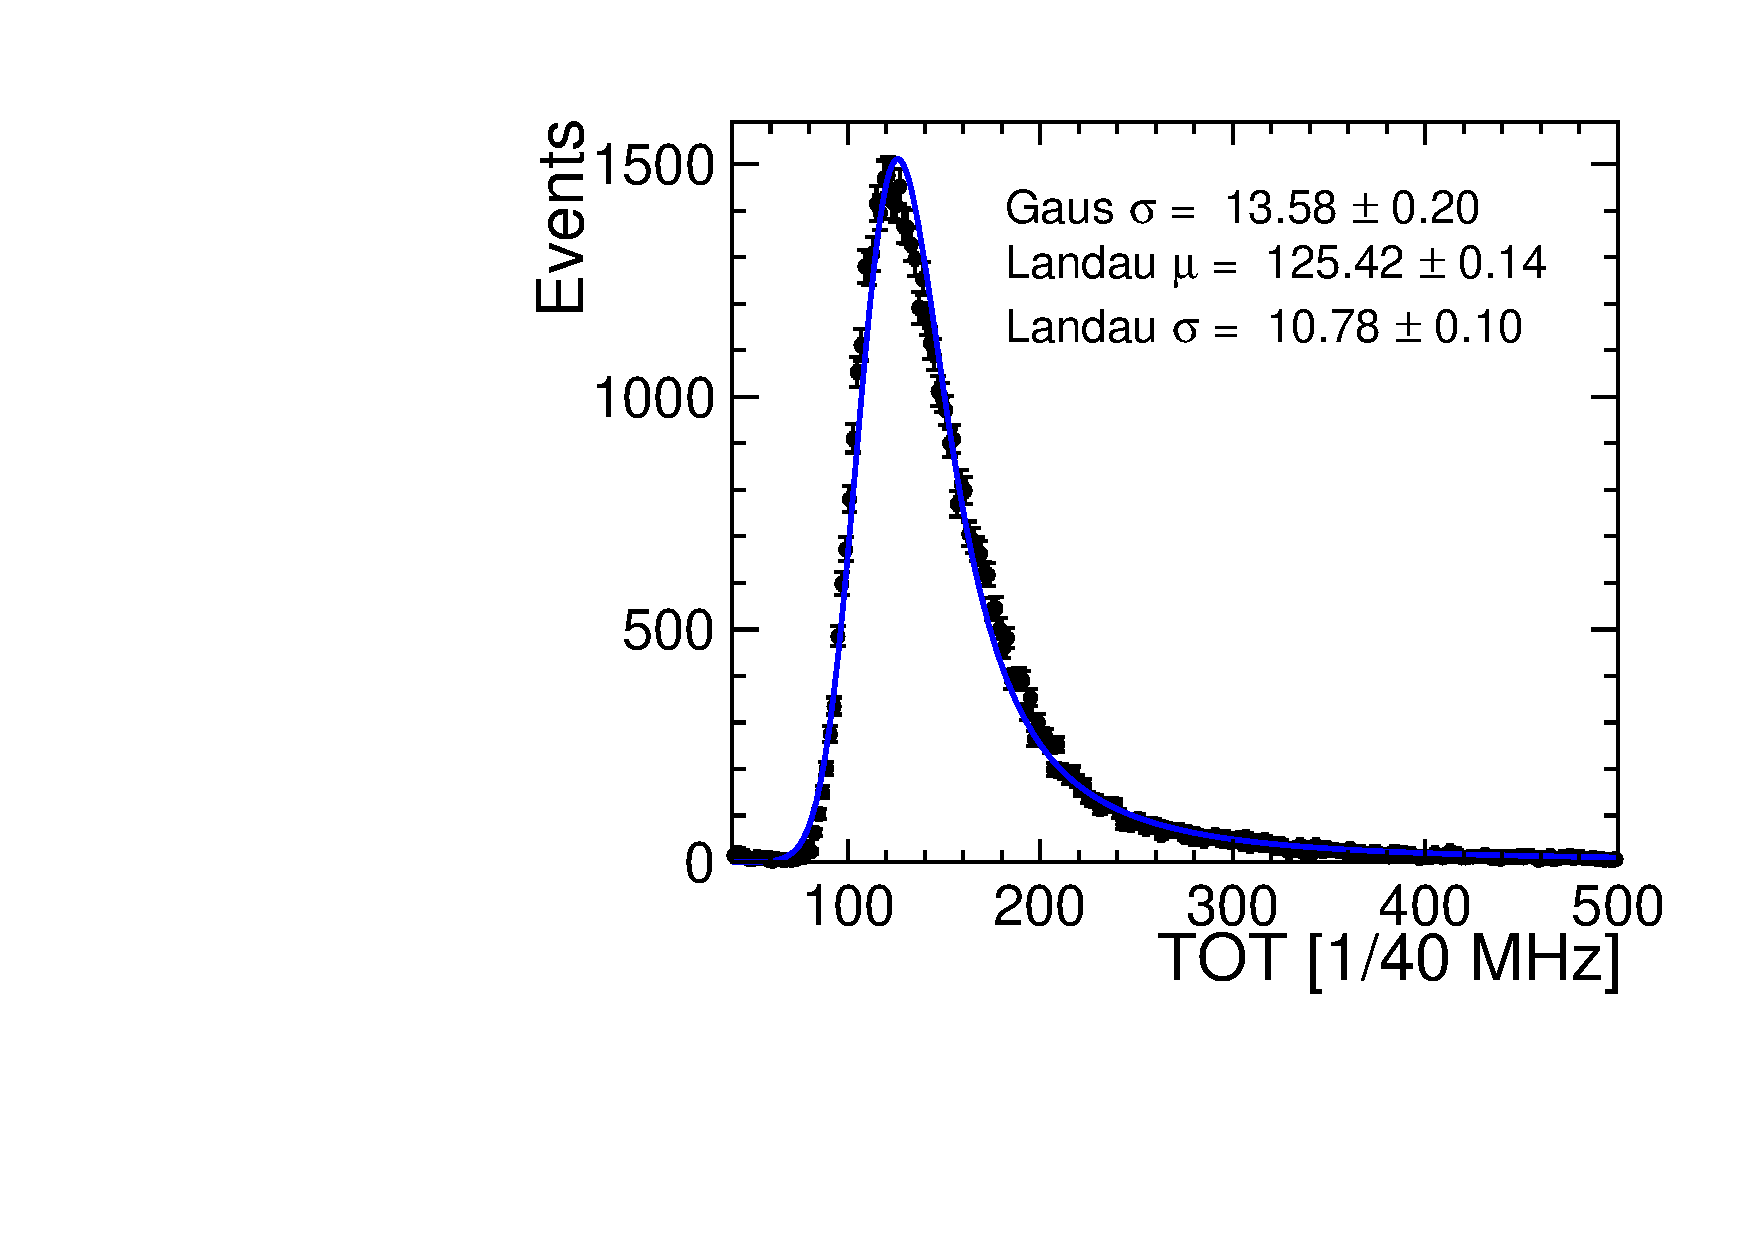
\includegraphics[width=\textwidth]{./figures/TestBeam/W2_J5_totalTOT_Langau_run1998.pdf}
  \caption{}\label{fig:W2_J5_DepletionVoltage_TOTdistr}
  \end{subfigure} \hfill
  \begin{subfigure}[b]{0.45\textwidth}
    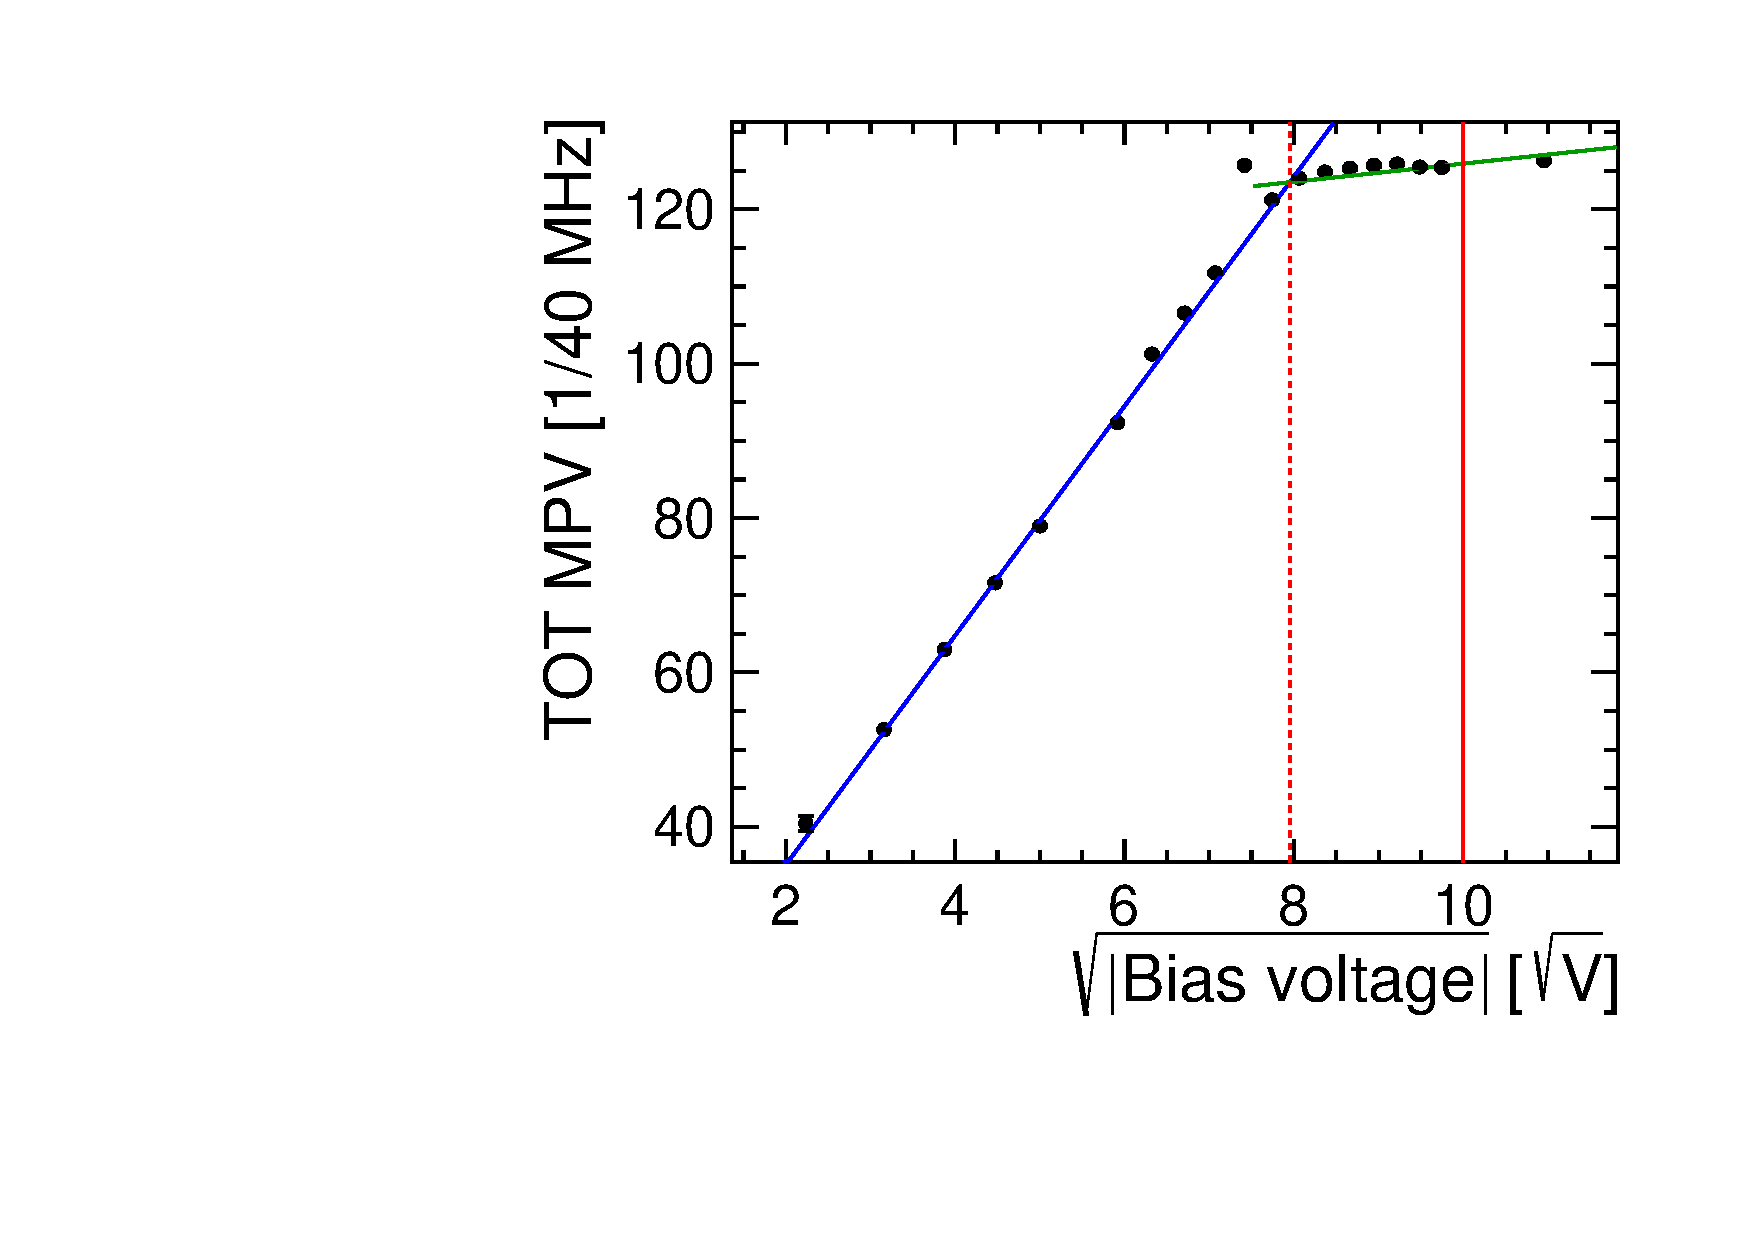
\includegraphics[width=\textwidth]{./figures/TestBeam/depletionVoltage_W0002_J05.pdf}
    \caption{}\label{fig:W2_J5_DepletionVoltage_chargeVSbiasVoltage}
  \end{subfigure}
  \caption{(a) The measured TOT distribution in a $300\,\micron$ thick
    silicon sensor (W2\_J5) with a bias voltage of 95~V fitted with a
    Landau function convoluted with a Gaussian function. (b) The most
    probable value of the measured TOT as a function of the bias
    voltage for W2\_J5. Straight lines are used to fit the slope and
    the plateau regions. The depletion voltage corresponds to the
    intersection of these two regions and shown in a red dashed
    line. The continuous red line shows the nominal operating bias
    voltage.}
  \label{fig:W2_J5_DepletionVoltage}
\end{figure}

\begin{table}[htbp]
  \centering
  \caption{Measured depletion voltage for the assemblies described in
    \cref{tab:Timepix3Assemblies} and calculated by fitting the
    plateau and slope regions of TOT as a function of the bias
    voltage.}
  \label{tab:depletionVoltage}
  \begin{tabular}{lc}
    \toprule
    Assembly & Depletion voltage [V] \\
    \midrule
    W19\_G7 & $<$-9.47 \\
    W19\_F7 & $<$-6.32 \\
    W19\_L8 & $<$-7.19\\
    W19\_C7 & $<$-5.43\\ \hline
    W5\_E2 & -10.82 \\ \hline
    W5\_F1 & -14.86 \\ \hline
    W2\_J5 & 63.23 \\ 
    \bottomrule
  \end{tabular}
\end{table}


\subsection{Charge sharing as a function of the track position}

The charge sharing is studied by extrapolating the track position
obtained from the Timepix3 telescope to the DUT. The size of the
clusters depends on the track position within the pixel. For the
perpendicular tracks to the DUT, multi-pixel clusters are created when
the track hits the edges or the corners of a pixel, leading to the
charge sharing between the pixel and its neighbouring pixels. The
charge sharing is also affected by the operating threshold of the
readout ASIC in addition to the track
position. \cref{fig:chargeSharingTrack} illustrates the track position
within the pixel for 1 to 4-pixel cluster sizes for a $50\,\micron$
sensor. For other thicknesses, the track position within the pixel is
shown in
\cref{fig:chargeSharingTrack_W19_G7,fig:chargeSharingTrack_W5_E2,fig:chargeSharingTrack_W5_F1}.

\begin{figure}[htbp] \centering
  \begin{subfigure}[b]{0.23\textwidth}
    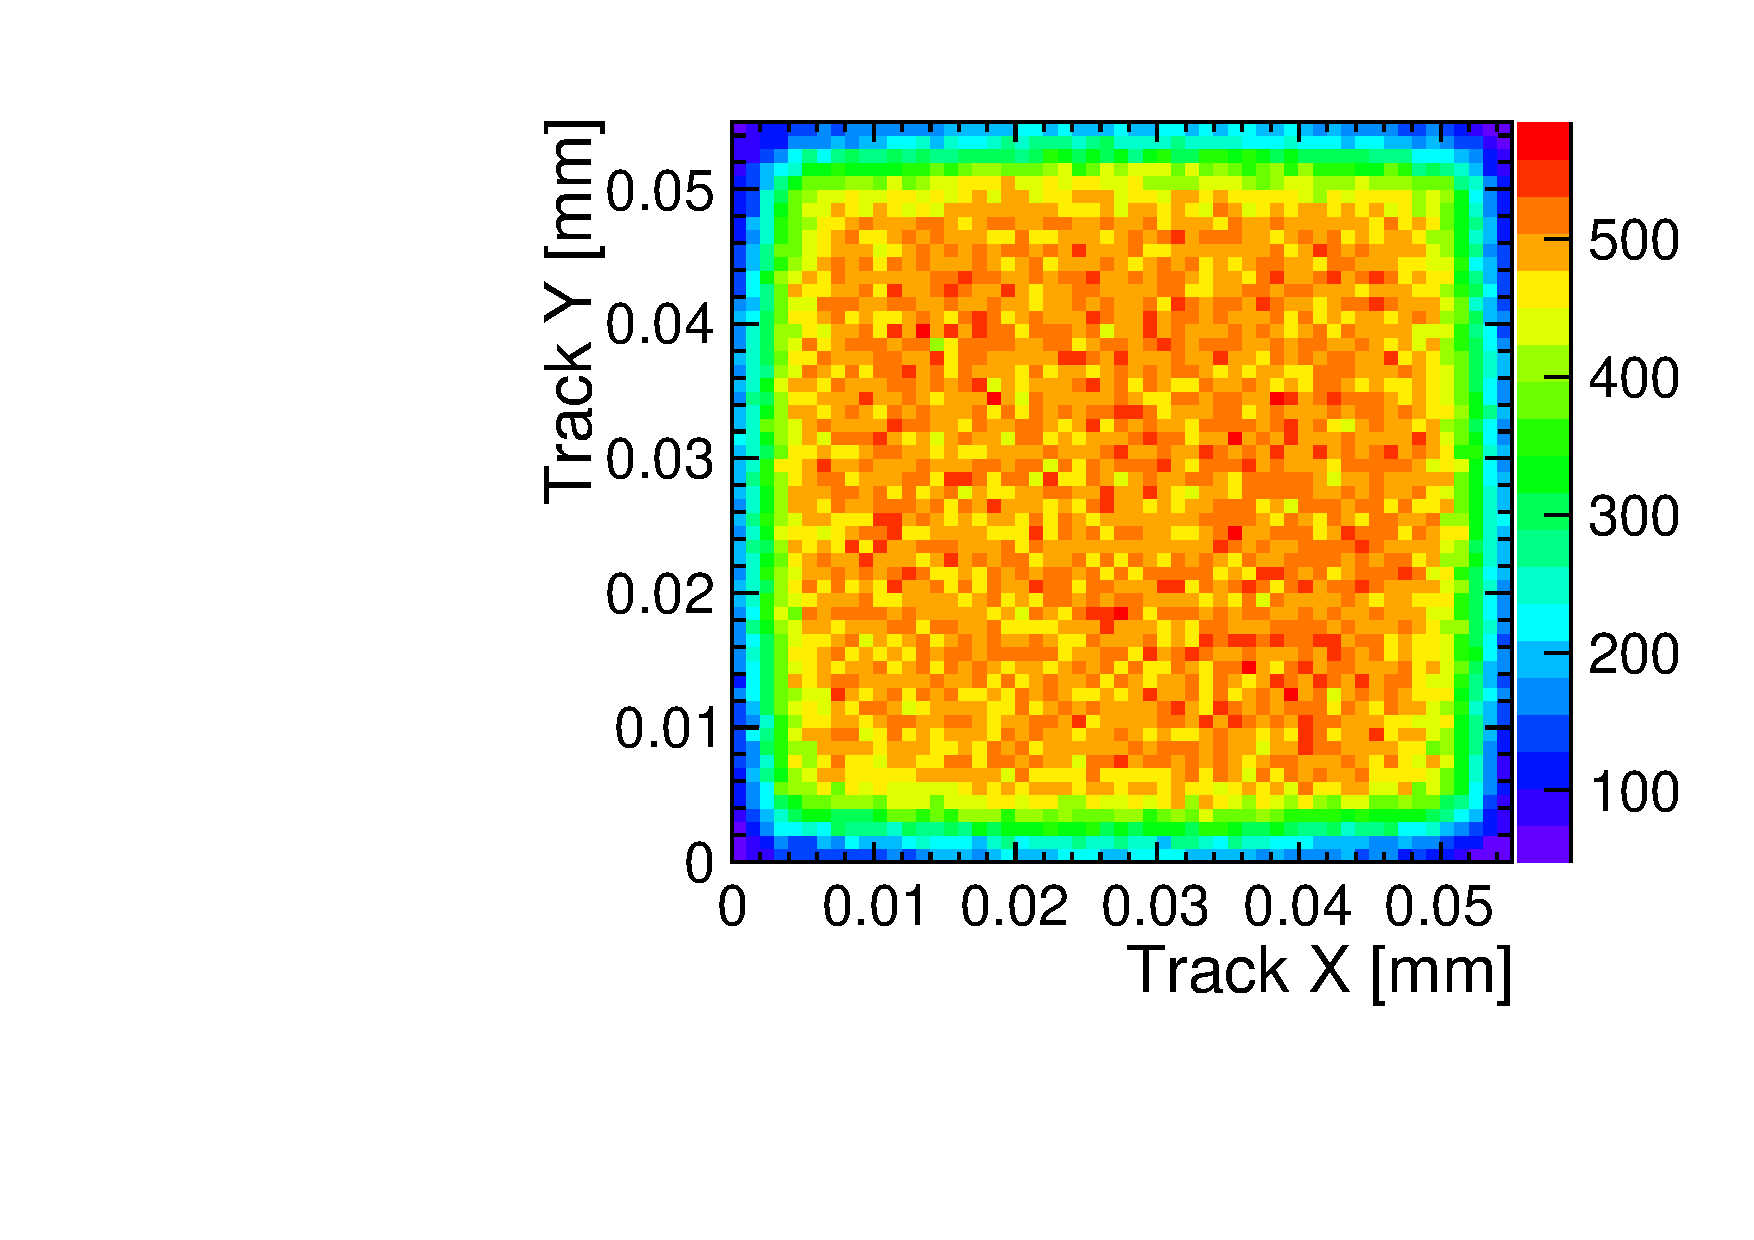
\includegraphics[width=\textwidth]{./figures/TestBeam/TrackPosWPixel_1hit_runW19_G7.pdf}
    \caption{Cluster size 1}
  \end{subfigure} \hfill
  \begin{subfigure}[b]{0.23\textwidth}
    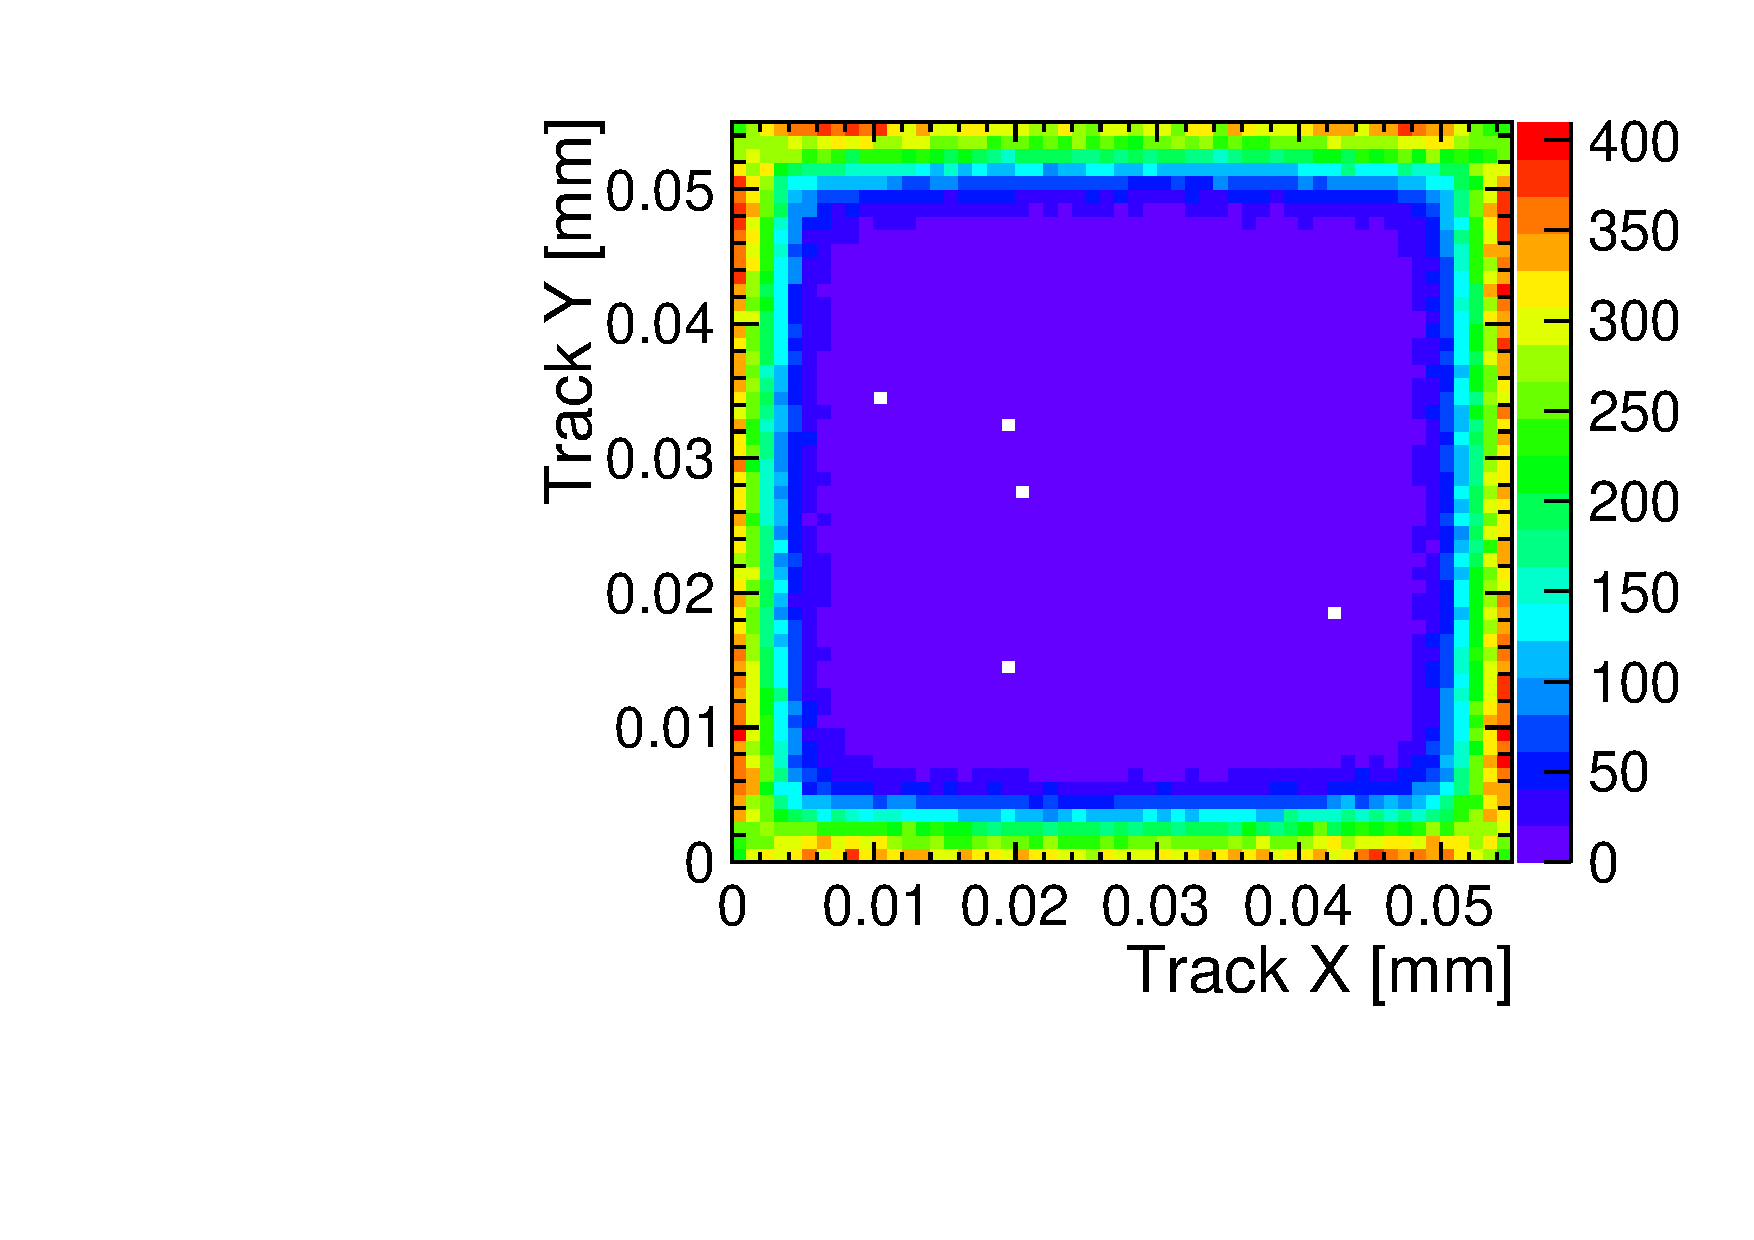
\includegraphics[width=\textwidth]{./figures/TestBeam/TrackPosWPixel_2hit_runW19_G7.pdf}
    \caption{Cluster size 2}
  \end{subfigure} \hfill
  \begin{subfigure}[b]{0.23\textwidth}
    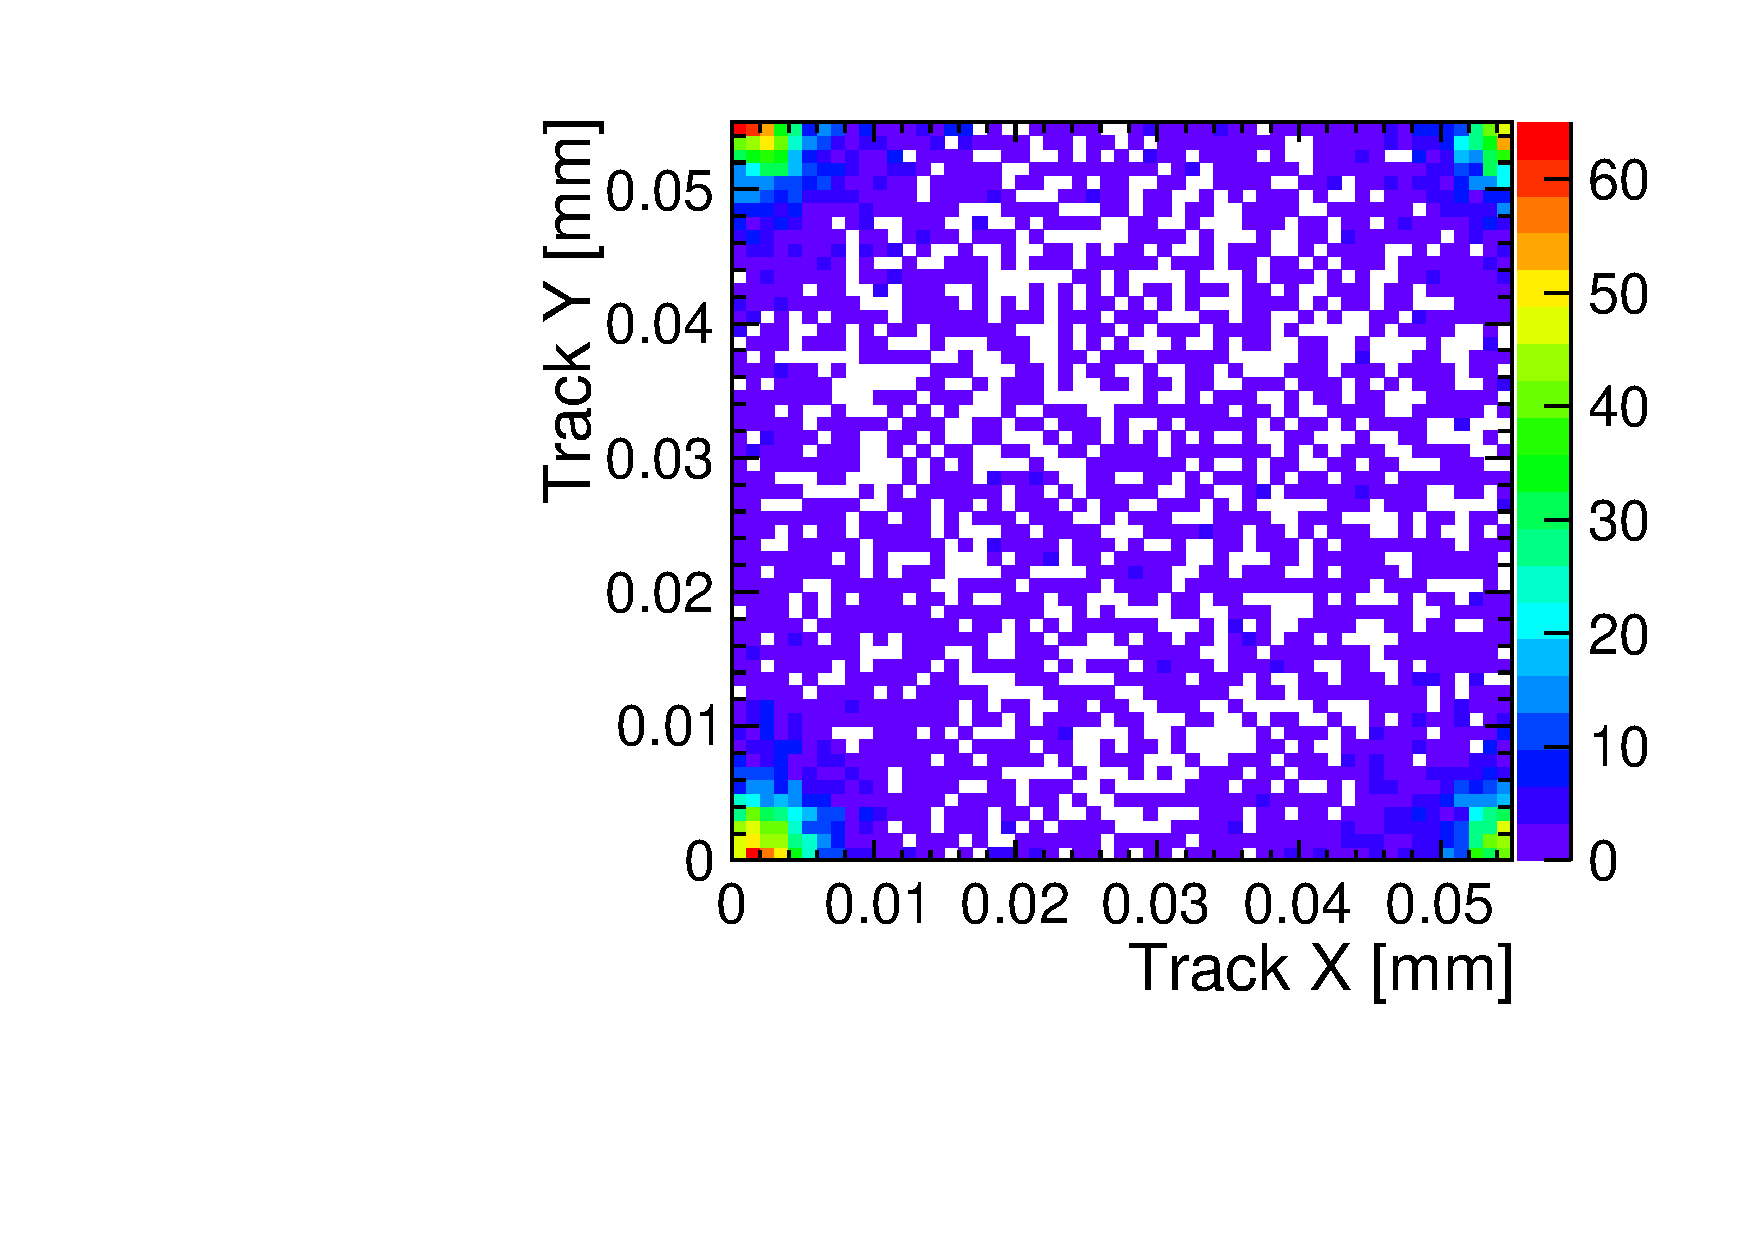
\includegraphics[width=\textwidth]{./figures/TestBeam/TrackPosWPixel_3hit_runW19_G7.pdf}
    \caption{Cluster size 3}
  \end{subfigure} \hfill
  \begin{subfigure}[b]{0.23\textwidth}
    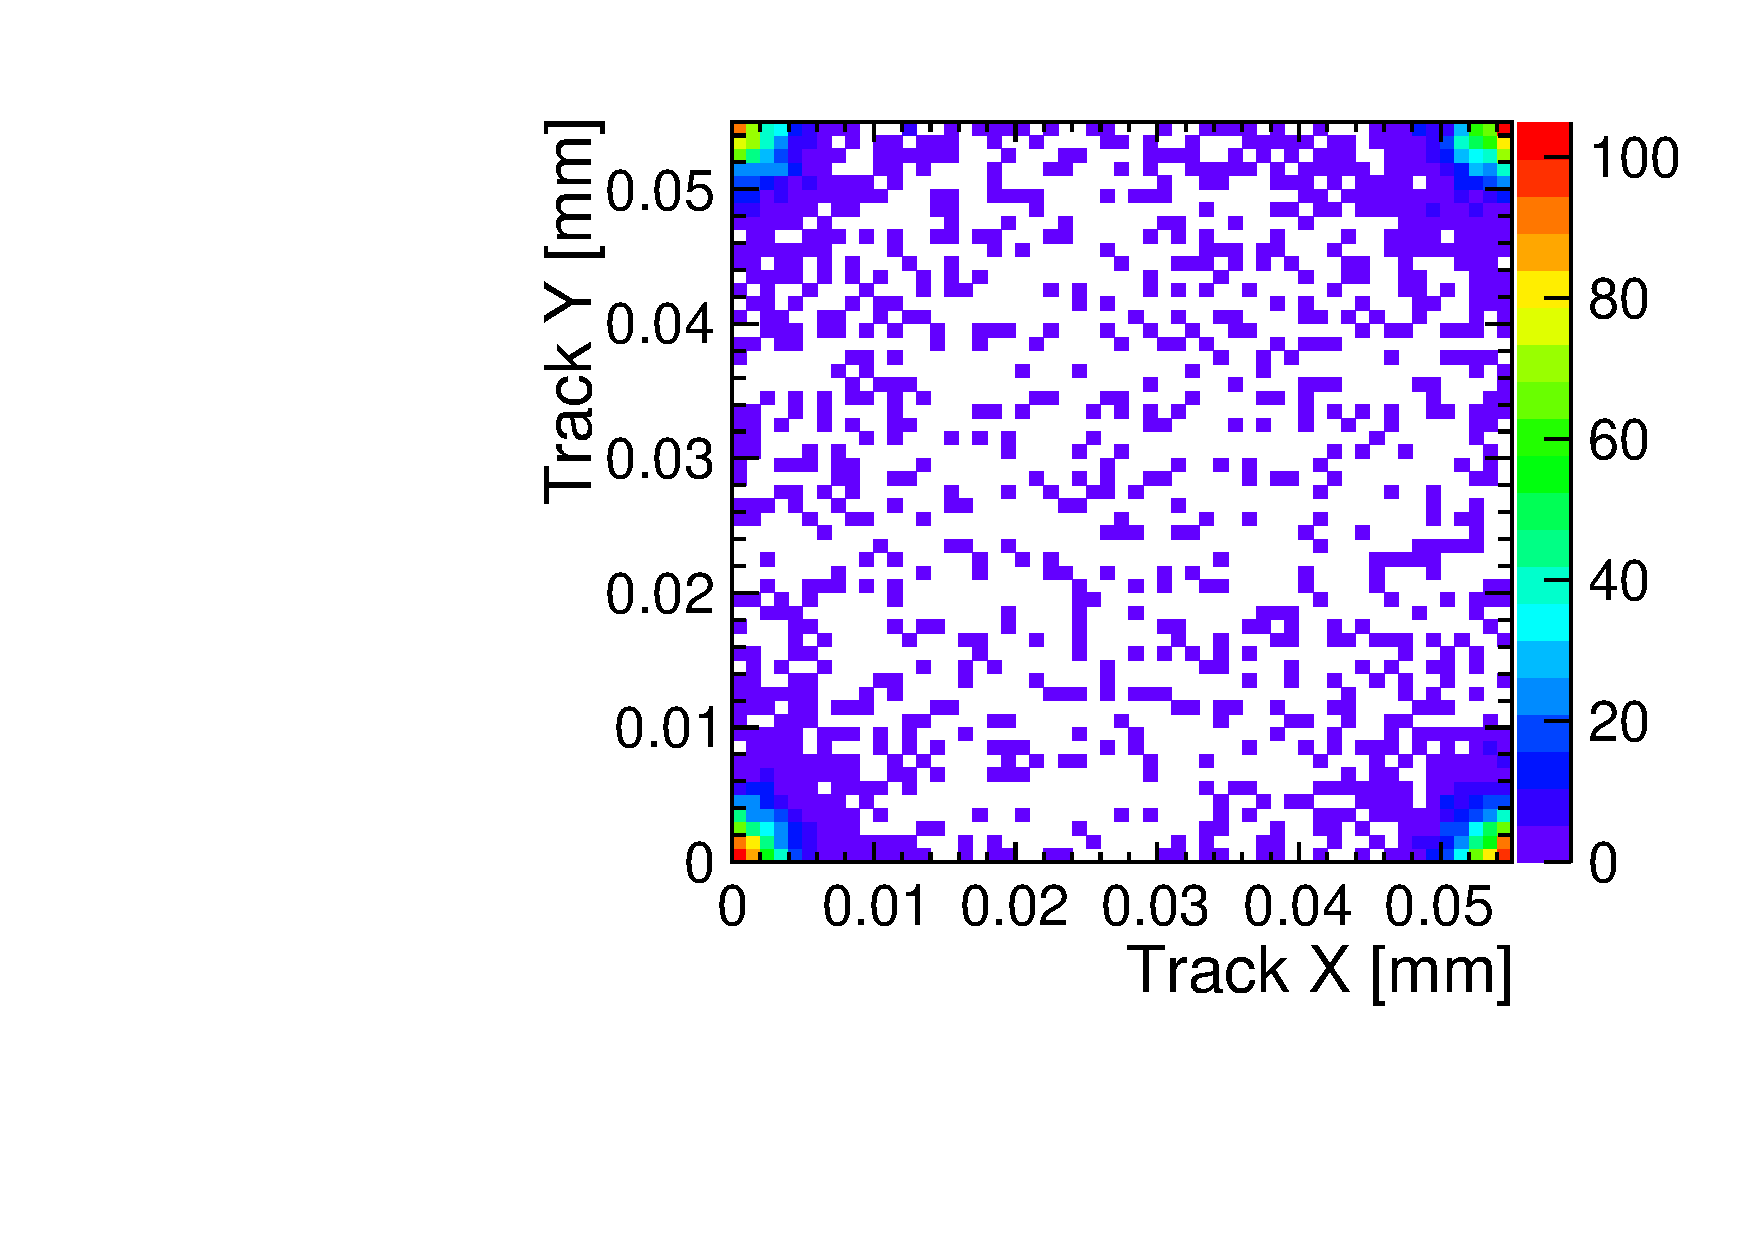
\includegraphics[width=\textwidth]{./figures/TestBeam/TrackPosWPixel_4hit_runW19_G7.pdf}
    \caption{Cluster size 4}
  \end{subfigure}
  \caption{Extrapolated track position within the pixel for 1 to 4-pixel
    cluster sizes for a $50\,\micron$ sensor (assembly W19\_G7). The
    assembly is operated at the nominal conditions.}
  \label{fig:chargeSharingTrack}
\end{figure}

\cref{fig:chargeSharing_2PC} compares the track position within the
pixel for two-pixel clusters in a one-dimensional profile for
different sensor thicknesses. The track position is closer to the
edges of the pixels to create a two-pixel clusters for thinner
sensors.

\begin{figure}[htbp] 
  \centering
  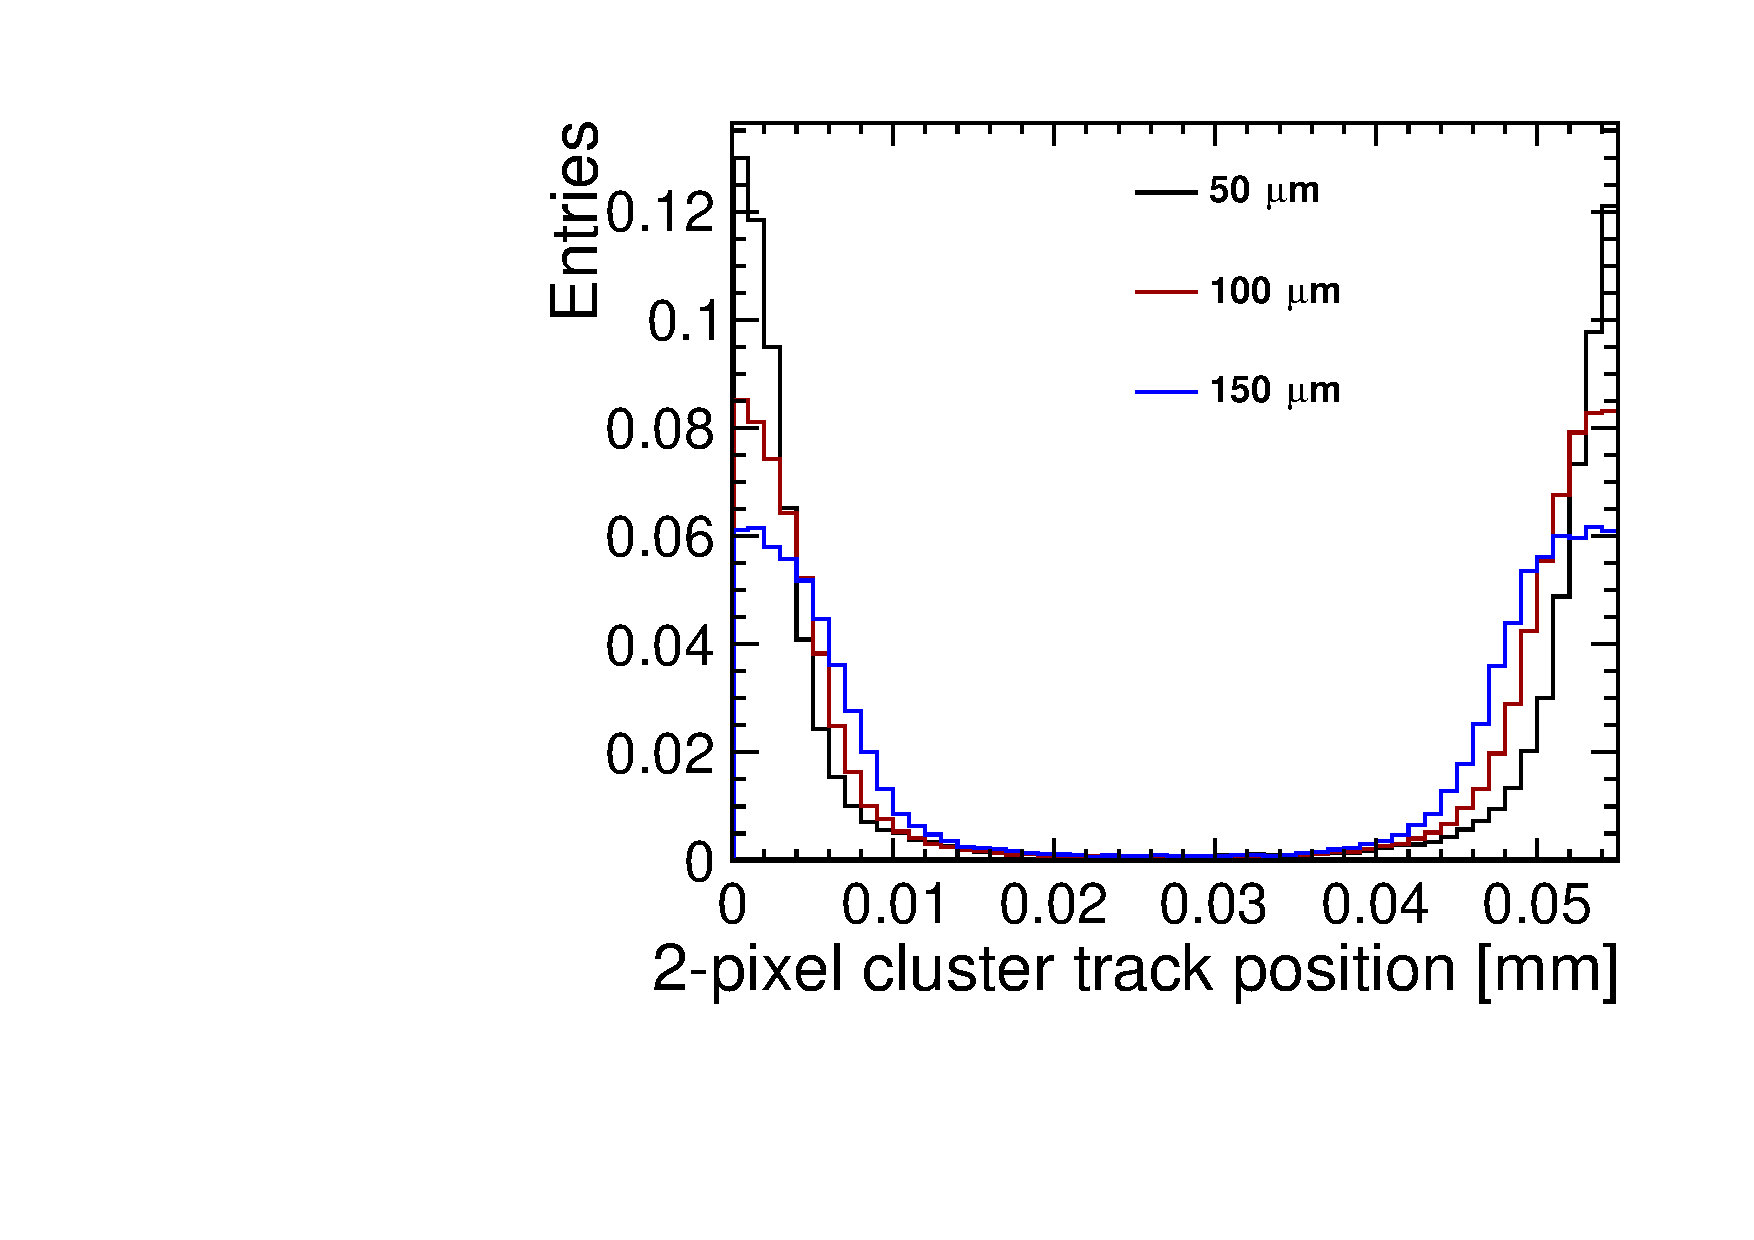
\includegraphics[width=0.5\textwidth]{./figures/TestBeam/chargeSharing_2pixel_clusters.pdf}
  \caption{Track position within the pixel for tracks leading to
    two-pixel clusters for different sensor thicknesses (the
    histograms are scaled to have a unit area).}
  \label{fig:chargeSharing_2PC}
\end{figure}

\subsection{Cluster size distribution}
The cluster size distribution is a straight indication on the amount
of charge sharing in a sensor. For thicker sensors, more charge
sharing is expected since the charge drifts in a longer distance and
diffuses across a larger transverse area. The threshold of the readout
electronics has a large impact on the detection of the charge
sharing. The threshold should be as low as possible to avoid
undetected energy deposits.

In this analysis, the hit pixels form a cluster with a distance
criterion of $\sqrt{2}$: pixels sharing common corners or edges are
considered as clusters. For sensor thicknesses in the range of
$50\,\micron$-$300\,\micron$, clusters of size one to four are
expected due to the charge sharing. Larger clusters are due to other
factors such as the $\delta$-rays.

The fraction of different cluster sizes depends on the operating
conditions of the assemblies like the bias voltage and the threshold
of the readout ASICs. \cref{fig:cluSize_operatingConditions} shows the
cluster size fraction for a $150\,\micron$ thick sensor (assembly
W5\_F1) operated at different bias voltages and thresholds.  

Higher bias voltages reduce the amount of charge sharing since the
drift time is lowered in a stronger electric field and the charges
diffuse less in the transverse direction. For very low bias voltages,
the sensor is under-depleted. An increase in bias voltage in this
regime increases the charge sharing. In fact, the pixel neighbouring a
hit pixel is more likely to be over threshold as more charge is
collected. The results for other assemblies are shown in
\cref{fig:clusterSize_vs_biasVoltage}.

Lowering the threshold leads to an increase in the cluster size
fraction distribution and thus a higher detection of the charge
sharing. Results for all the assemblies are shown in
\cref{fig:clusterSize_vs_THLscan}.


\begin{figure}[htbp] \centering
  \begin{subfigure}[b]{0.45\textwidth}
    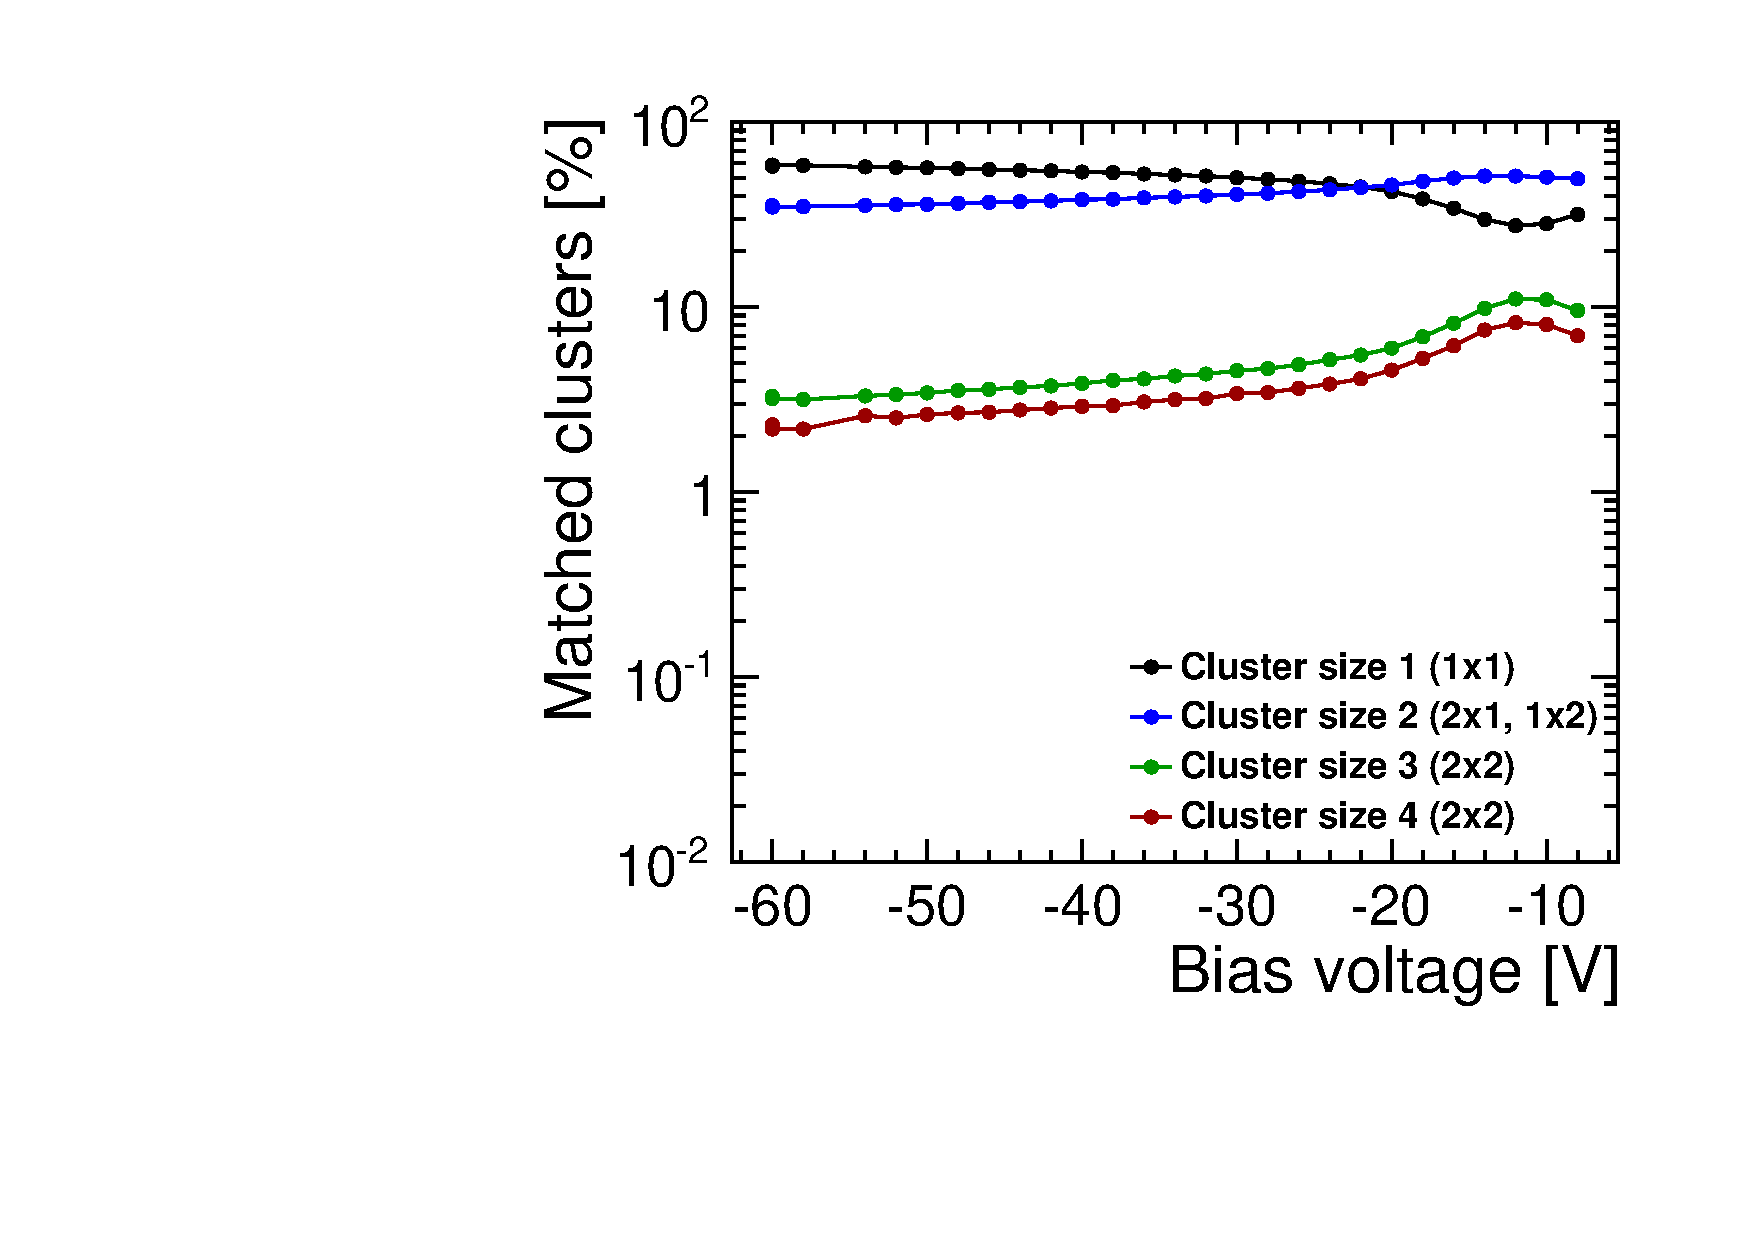
\includegraphics[width=\textwidth]{./figures/TestBeam/cluSize_biasScan_W0005_F01.pdf}
    \caption{}
  \end{subfigure} \hfill
  \begin{subfigure}[b]{0.45\textwidth}
    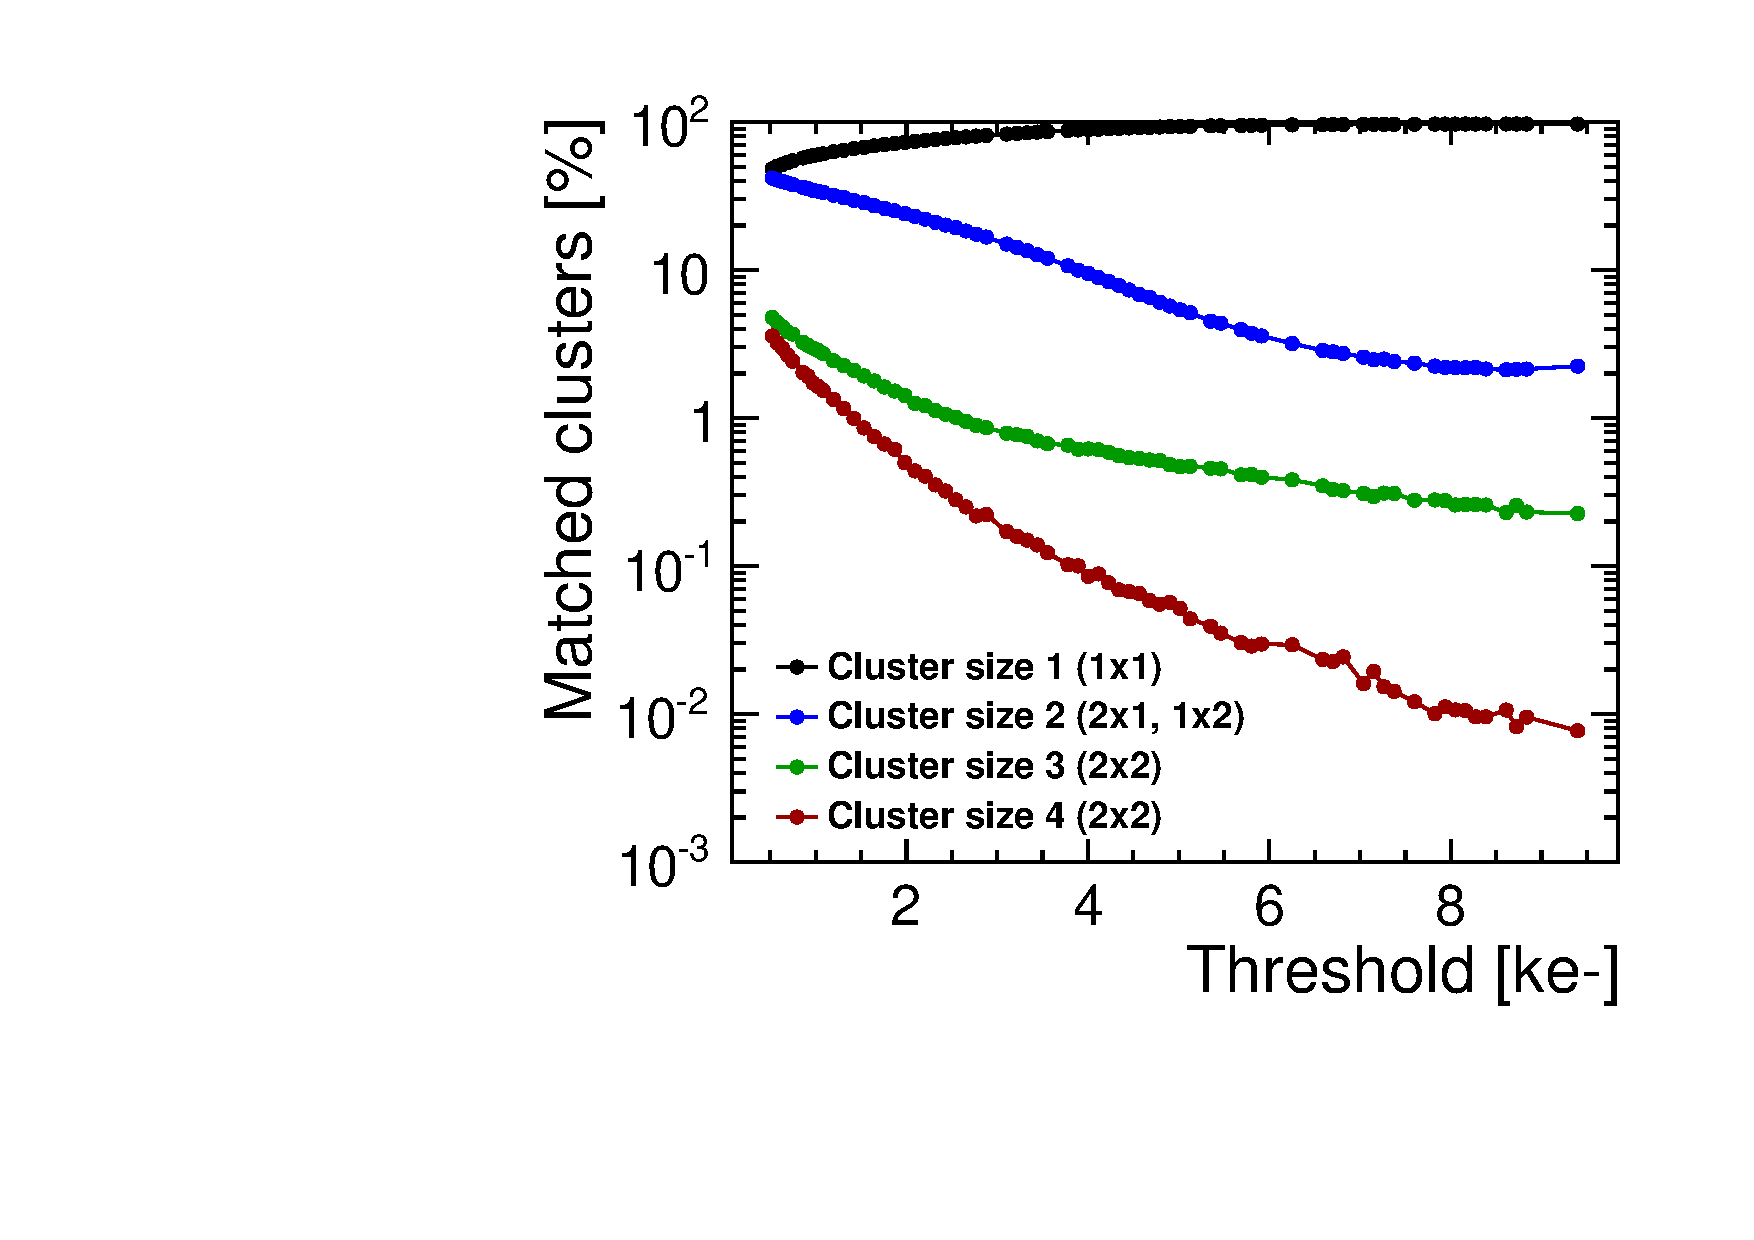
\includegraphics[width=\textwidth]{./figures/TestBeam/cluSize_THLscan_W0005_F01.pdf}
    \caption{}
  \end{subfigure}
  \caption{Fraction of cluster sizes as a function of (a) bias voltage
    and (b) threshold for the assembly W5\_F1 with a $150\,\micron$
    thick sensor.}
  \label{fig:cluSize_operatingConditions}
\end{figure}


The cluster size fraction as a function of the sensor thickness for
data recorded at the nominal operating conditions is shown in
\cref{fig:cluSize_thickness}. Charge sharing increases with sensor
thickness. The fraction of $1\times2$ and $2\times1$-pixel clusters are
very similar for square pixels and 2-pixel clusters combine these two
cluster geometries.

\begin{figure}[htbp] 
  \centering
  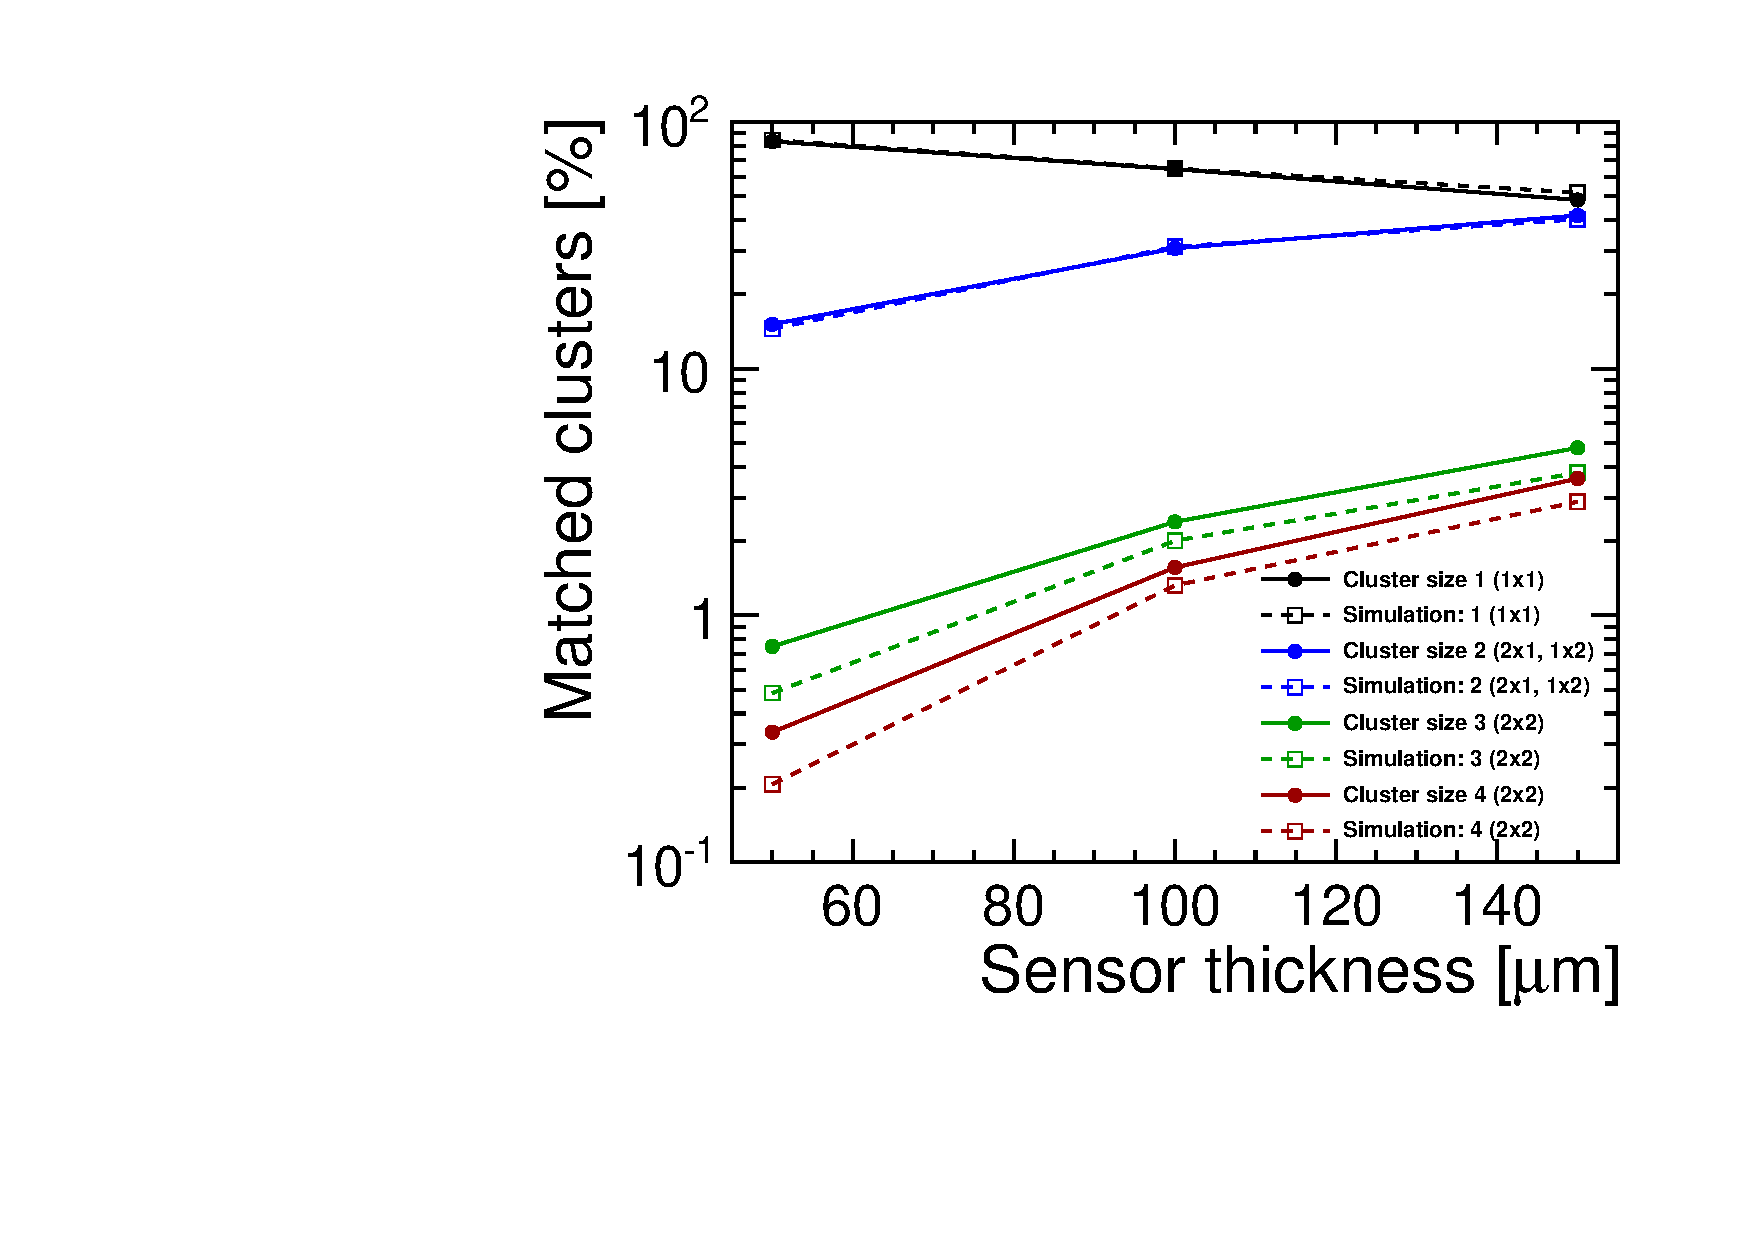
\includegraphics[width=0.5\textwidth]{./figures/TestBeam/cluSize_vs_thickness.pdf}
  \caption{Fraction of different cluster sizes as a function of sensor
    thickness for runs recorded under nominal operating conditions.}
  \label{fig:cluSize_thickness}
\end{figure}

\subsection{Single-point resolution}

From the test-beam data, the residuals are calculated by comparing the
reconstructed hit position with the extrapolated track position
obtained by the telescope. This residual combines in quadrature the
single-point (or hit) and the track resolutions:

\begin{equation}
  \sigma_{\mathrm{residual}}^{2}=\sigma_{\mathrm{hit}}^{2}+\sigma_{\mathrm{track}}^{2} .
  \label{eq:residualEq}
\end{equation}

In the following, the tracking resolution is not unfolded from the
residual measurements presented. For the estimation of the
single-point resolution, the tracking resolution of $\sim2\,\micron$
at the SPS test beam should be unfolded (c.f.~\cref{ch:Telescope}).

The residuals depend highly on the cluster sizes since the
reconstructed hit position takes into account the number of the hit
pixels in a cluster and the charge information in each
pixel. \cref{fig:residuals_cluSize} illustrates the residuals for the
a $50\,\micron$ thick sensor (assembly W19\_G7) for different cluster
sizes. For single-pixel clusters, the hit position corresponds to the
geometric center of the pixel and therefore a resolution of pixel
pitch$/\sqrt{12}$ is expected (as explained in
\cref{sec:binaryReadout}). For multi-pixel clusters, by using the
charge information, a more accurate interpolation of the hit position
can be obtained and the resolution is better than the geometrical
information (by using the $\eta$-correction method as described in
\cref{sec:EtaCorrection}).

\begin{figure}[htbp] \centering
  \begin{subfigure}[b]{0.23\textwidth}
    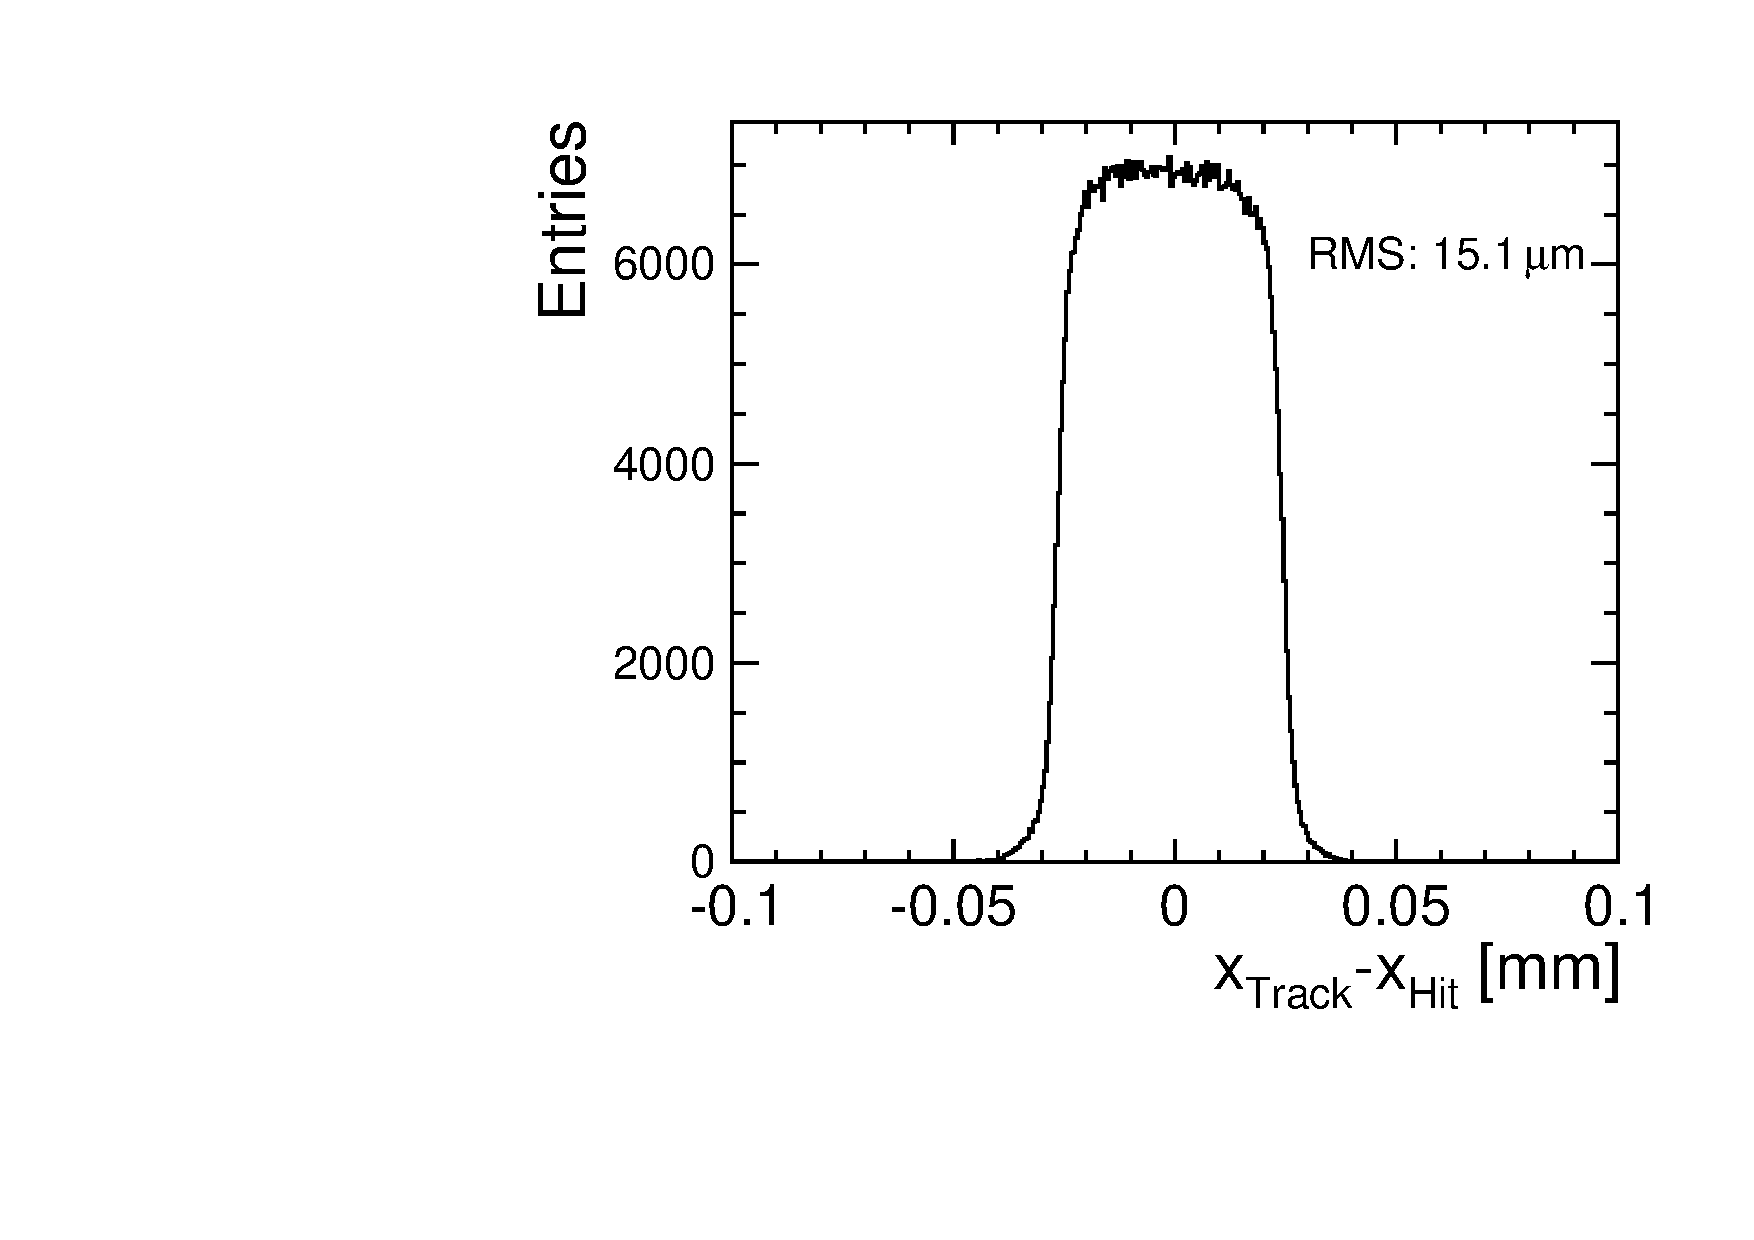
\includegraphics[width=\textwidth]{./figures/TestBeam/residual_1hit_W19_G7.pdf}
    \caption{Cluster size 1}
  \end{subfigure} \hfill
  \begin{subfigure}[b]{0.23\textwidth}
    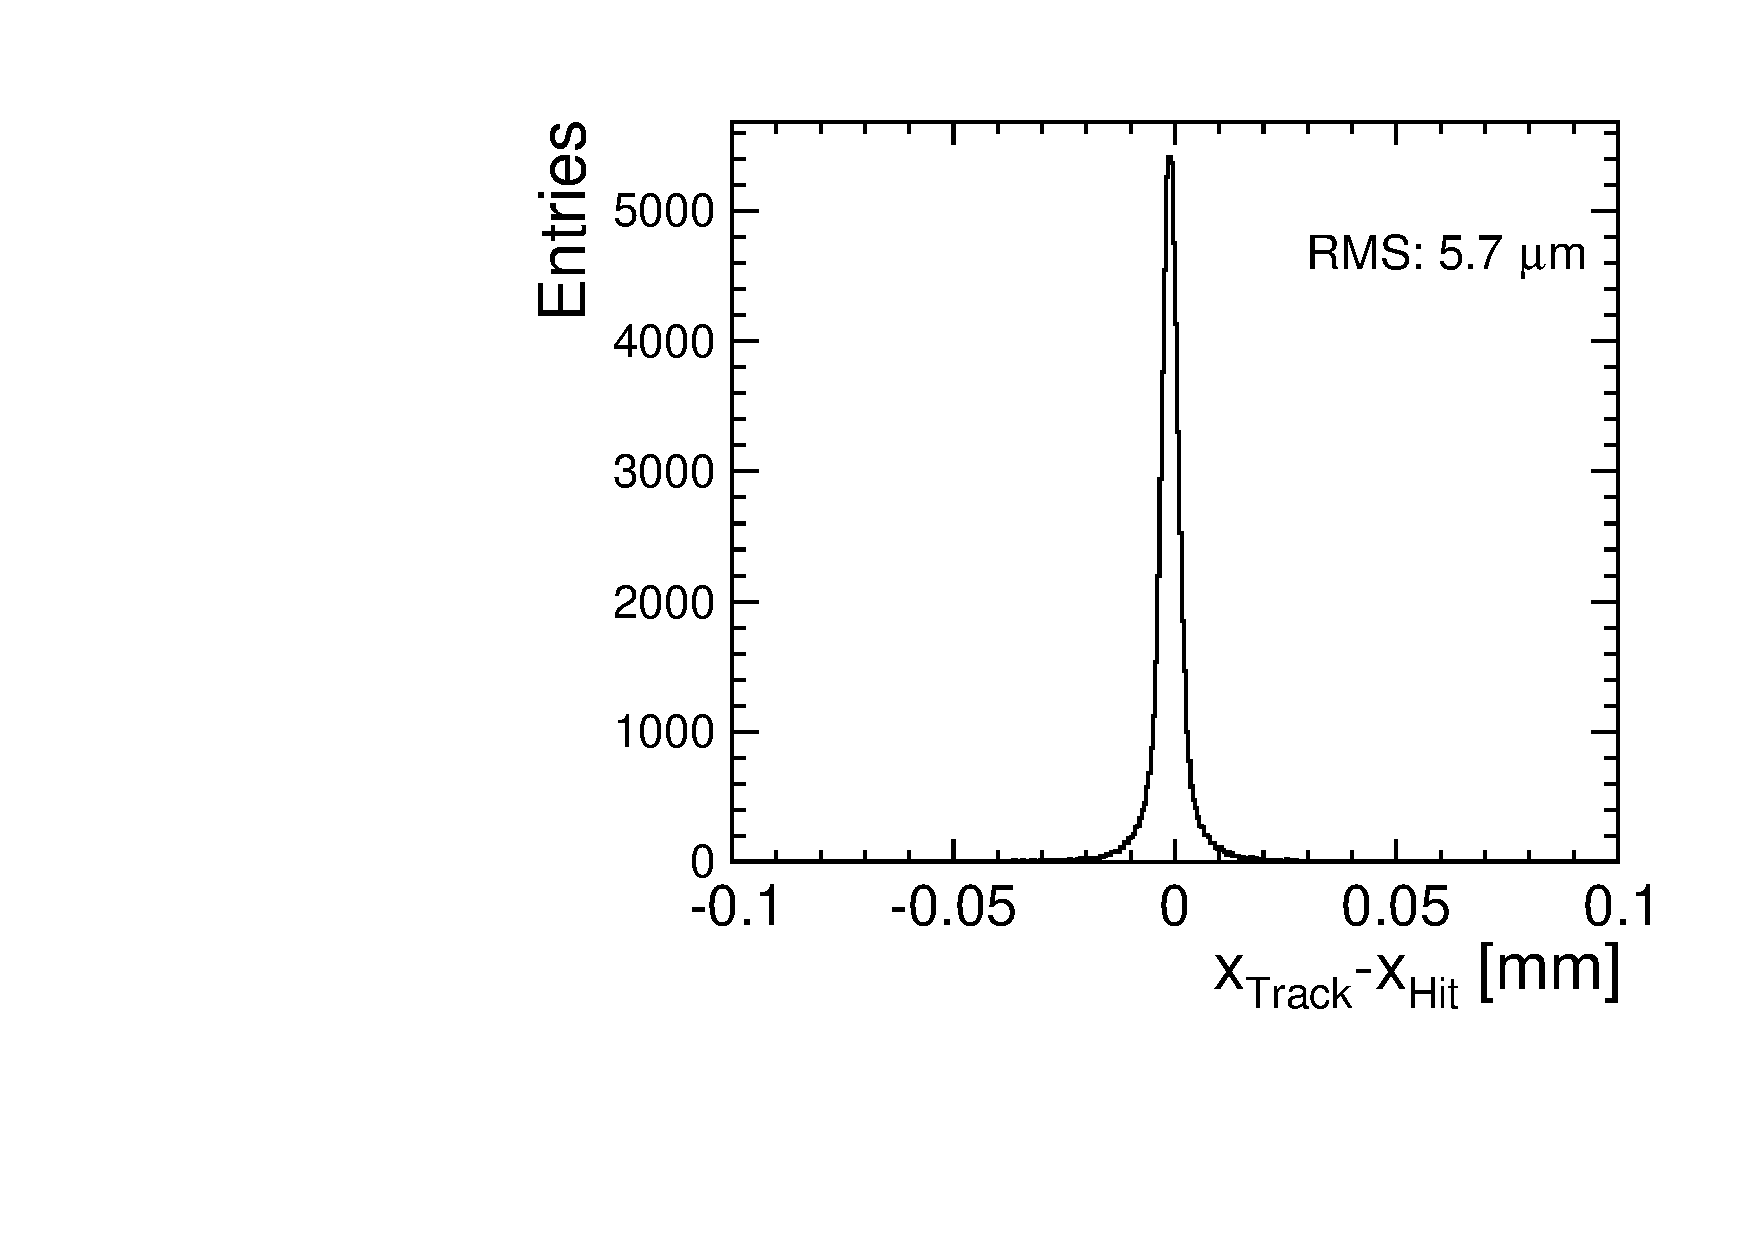
\includegraphics[width=\textwidth]{./figures/TestBeam/residual_2hit_W19_G7.pdf}
    \caption{Cluster size 2}
  \end{subfigure} \hfill
  \begin{subfigure}[b]{0.23\textwidth}
    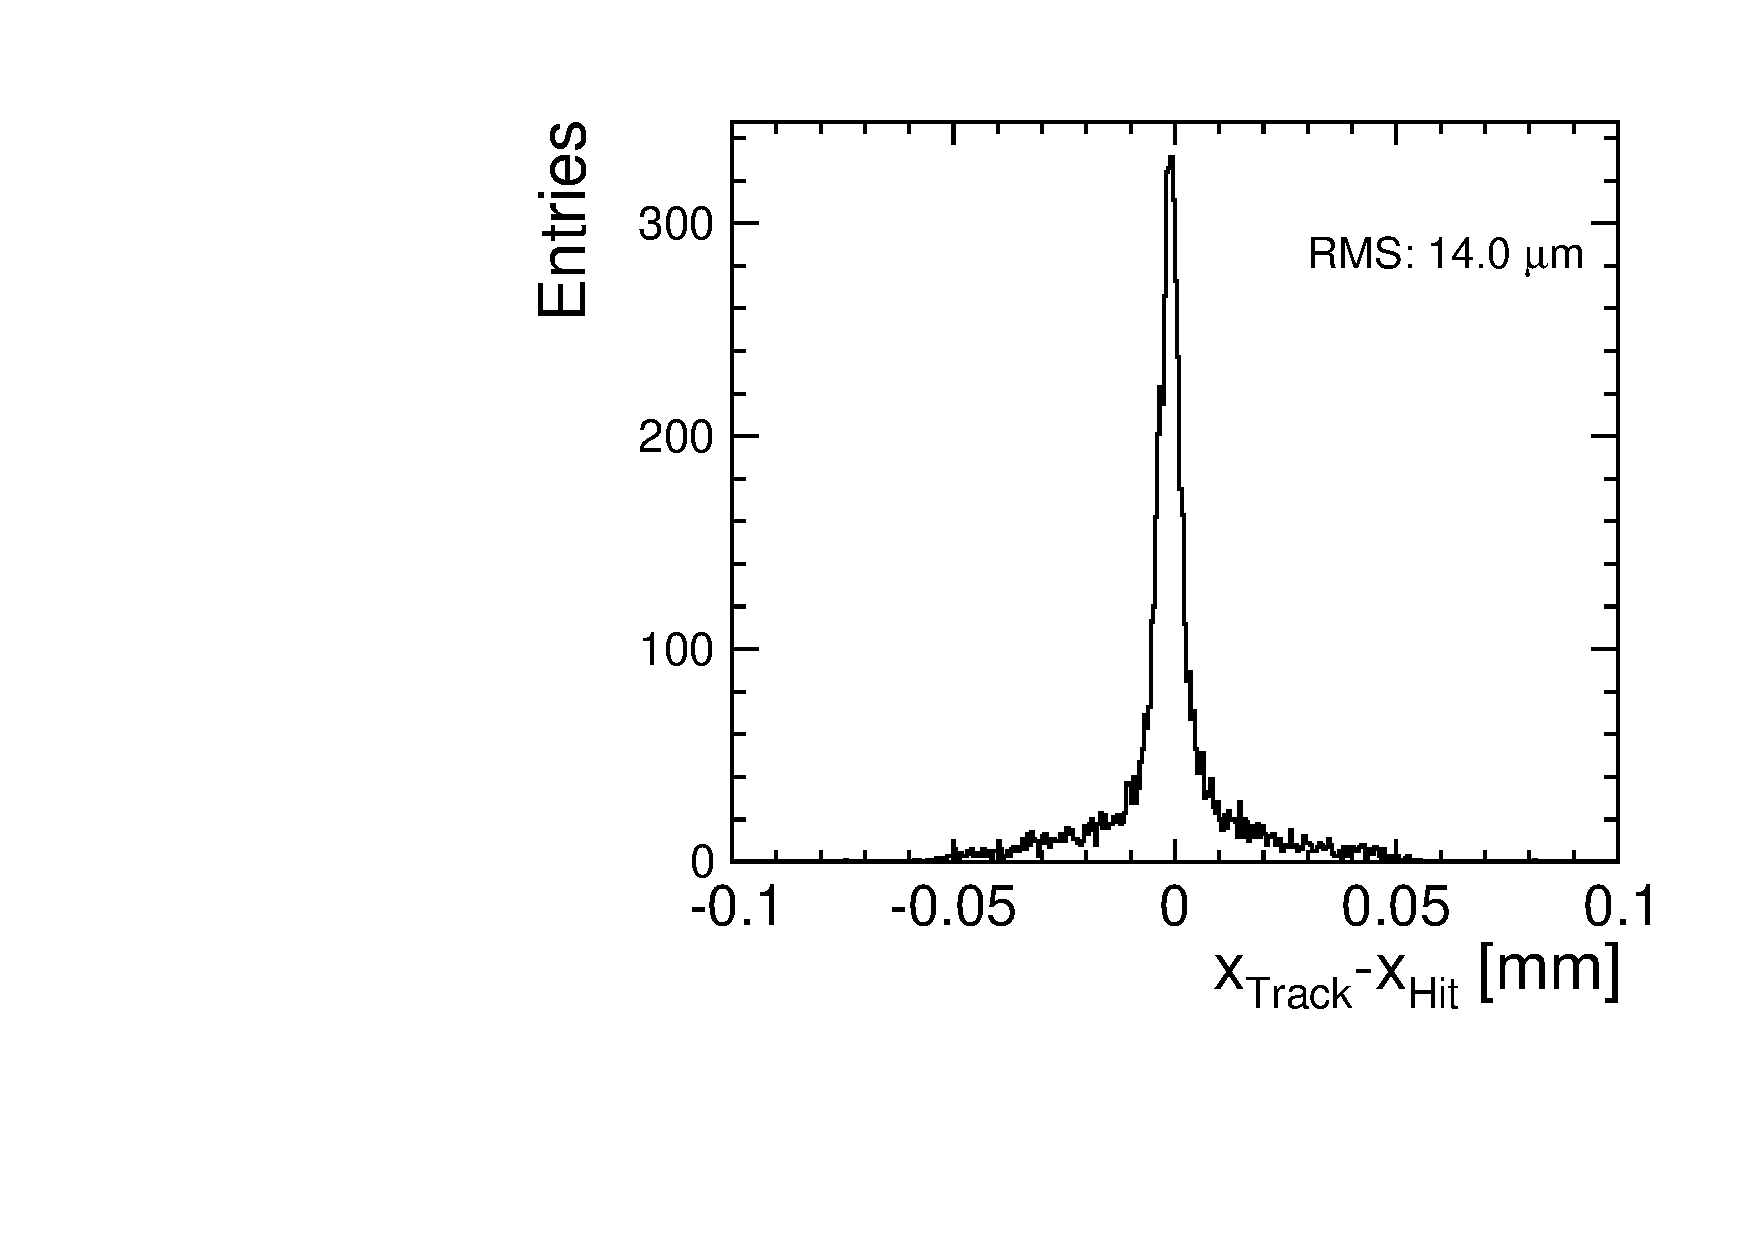
\includegraphics[width=\textwidth]{./figures/TestBeam/residual_3hit_W19_G7.pdf}
    \caption{Cluster size 3}
  \end{subfigure} \hfill
  \begin{subfigure}[b]{0.23\textwidth}
    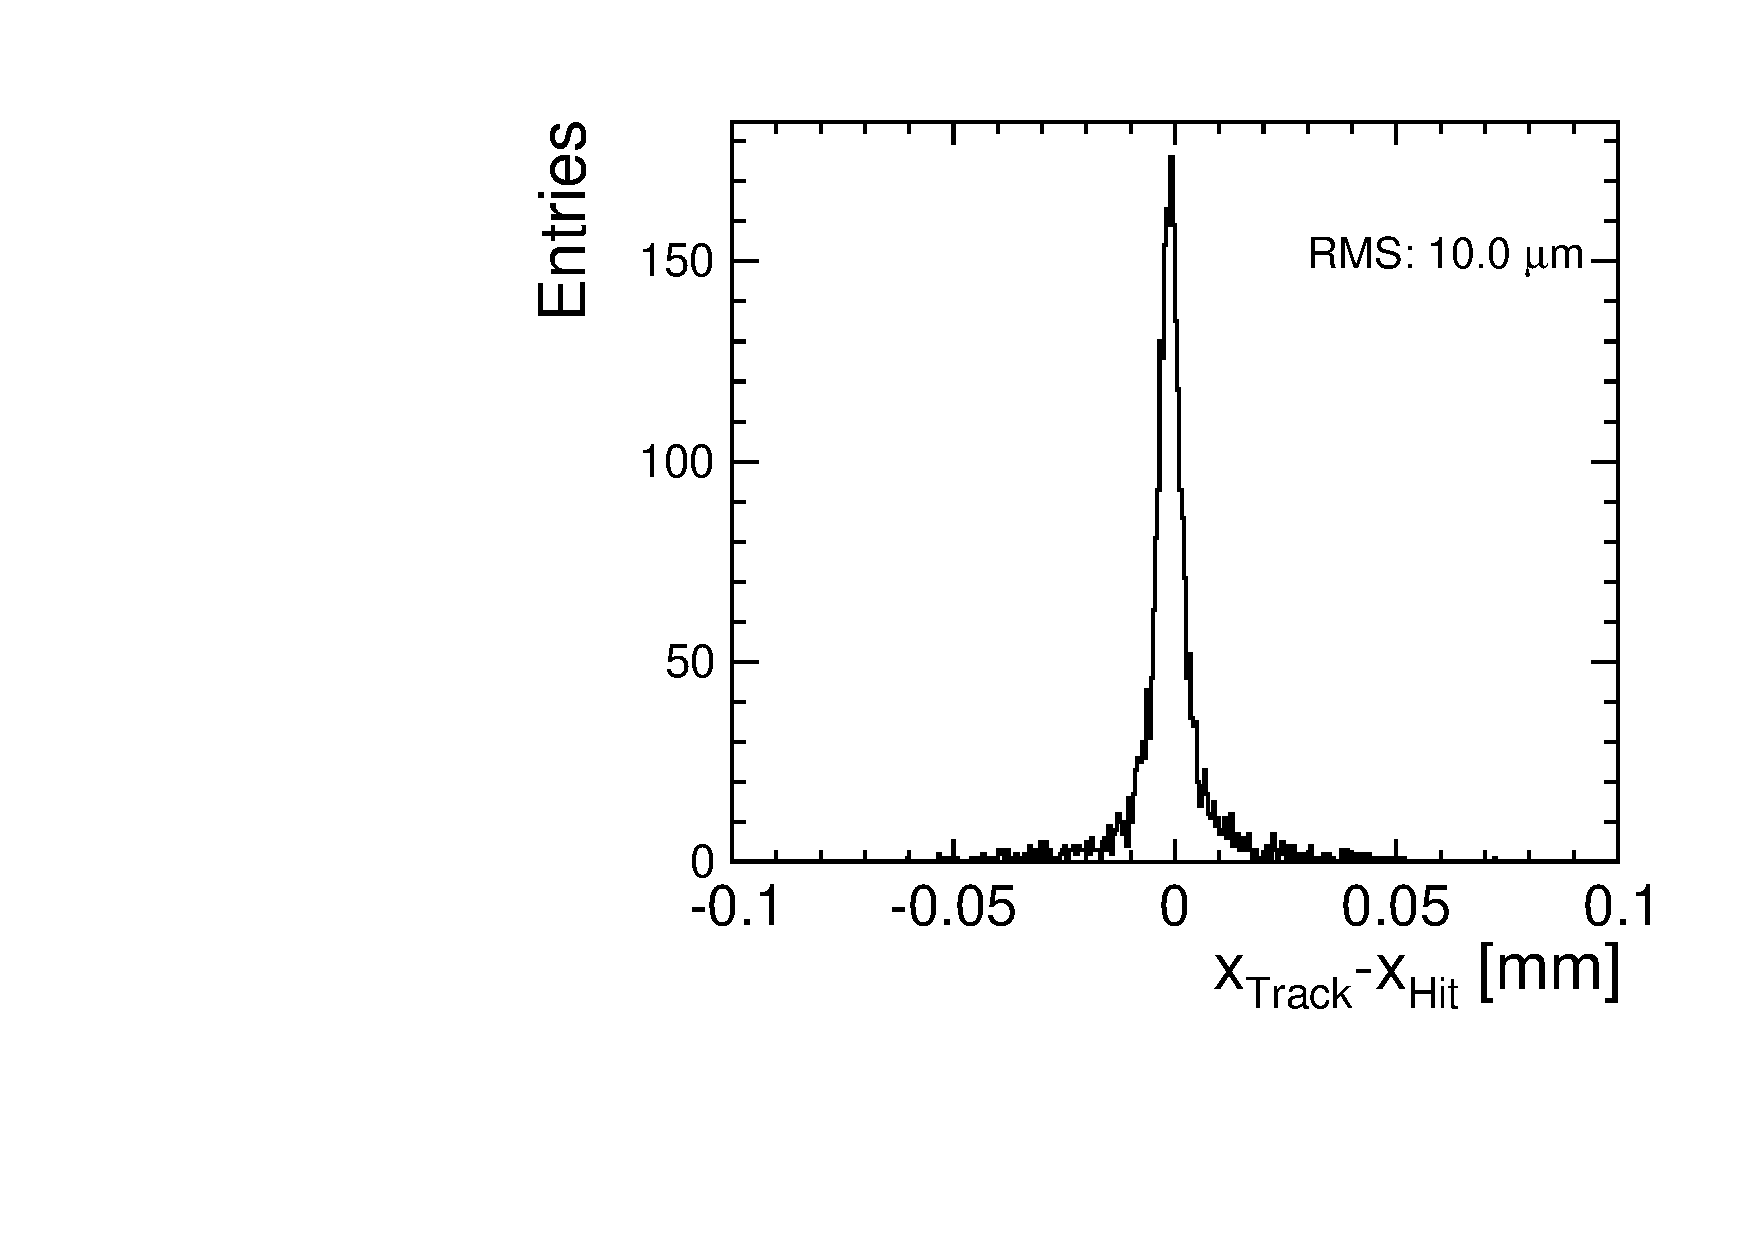
\includegraphics[width=\textwidth]{./figures/TestBeam/residual_4hit_W19_G7.pdf}
    \caption{Cluster size 4}
  \end{subfigure}
  \caption{The residuals for a $50\,\micron$ thick sensor (assembly
    W19\_G7) for different cluster sizes: (a) Cluster size 1
    ($1\times1$), (b) Cluster size 2 ($2\times1$), (c) Cluster size 3
    ($2\times2$) and (d) Cluster size 4 ($2\times2$). The track
    resolution is not unfolded.}
  \label{fig:residuals_cluSize}
\end{figure}

The overall residual is defined by the average of the residual of each
cluster size weighted by the relative fractions of different cluster
sizes. The factors affecting the fraction of different cluster sizes
such as the sensor thickness and the operating conditions of the
assembly (threshold and bias voltage) affect as well the
residuals. \cref{fig:Residuals_bias_threshold} shows the RMS of the
residuals in the x and y directions for a $50\,\micron$ thick sensor
(assembly W19\_G7) as a function of the bias voltage and the
threshold. For other assemblies, these plots are shown in
\cref{fig:Residuals_vs_biasVoltage,fig:Residuals_vs_Threshold}. The
residuals follow the same trend as the cluster size distributions:
higher fractions of single-hit clusters result in higher residuals.


\begin{figure}[htbp] \centering
  \begin{subfigure}[b]{0.45\textwidth}
    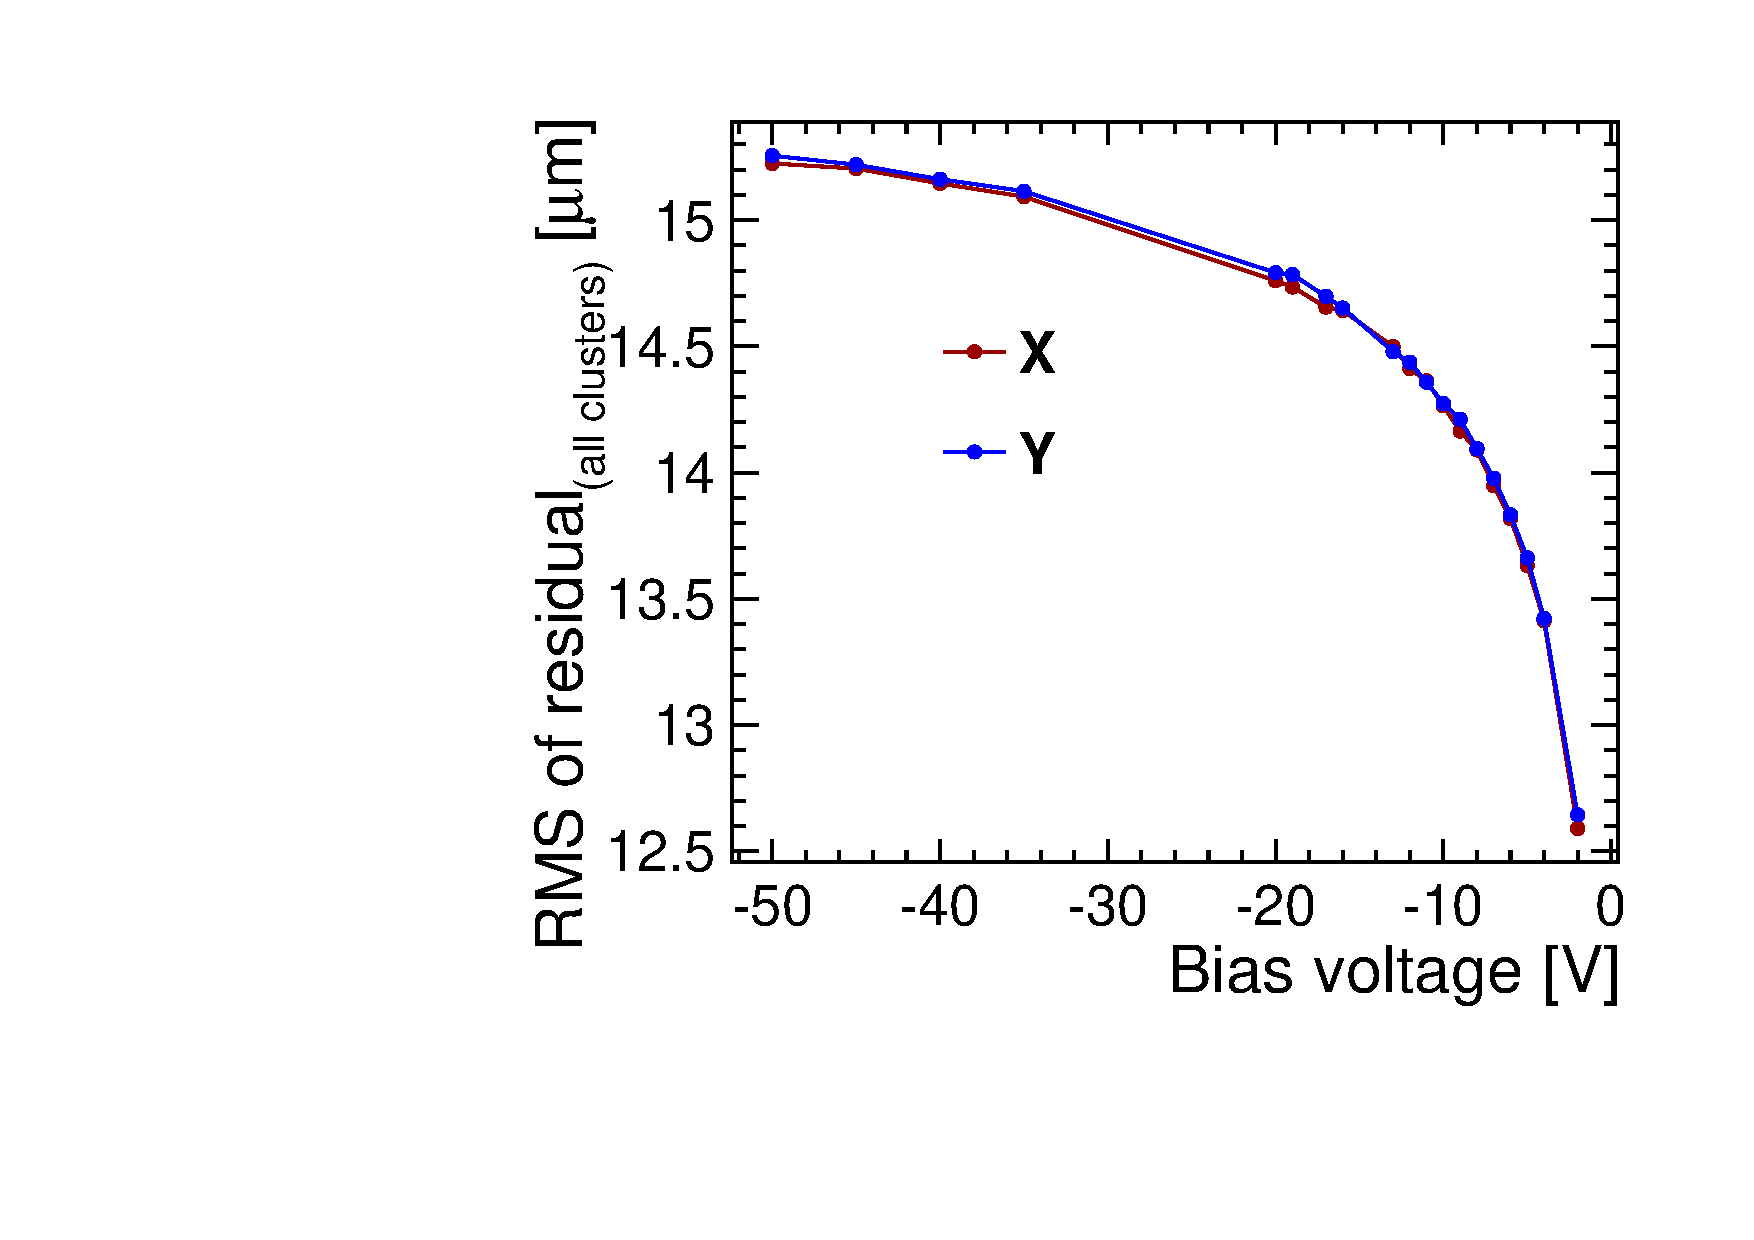
\includegraphics[width=\textwidth]{./figures/TestBeam/W19_G7_Residual_vs_bias.pdf}
    \caption{}
  \end{subfigure} \hfill
  \begin{subfigure}[b]{0.45\textwidth}
    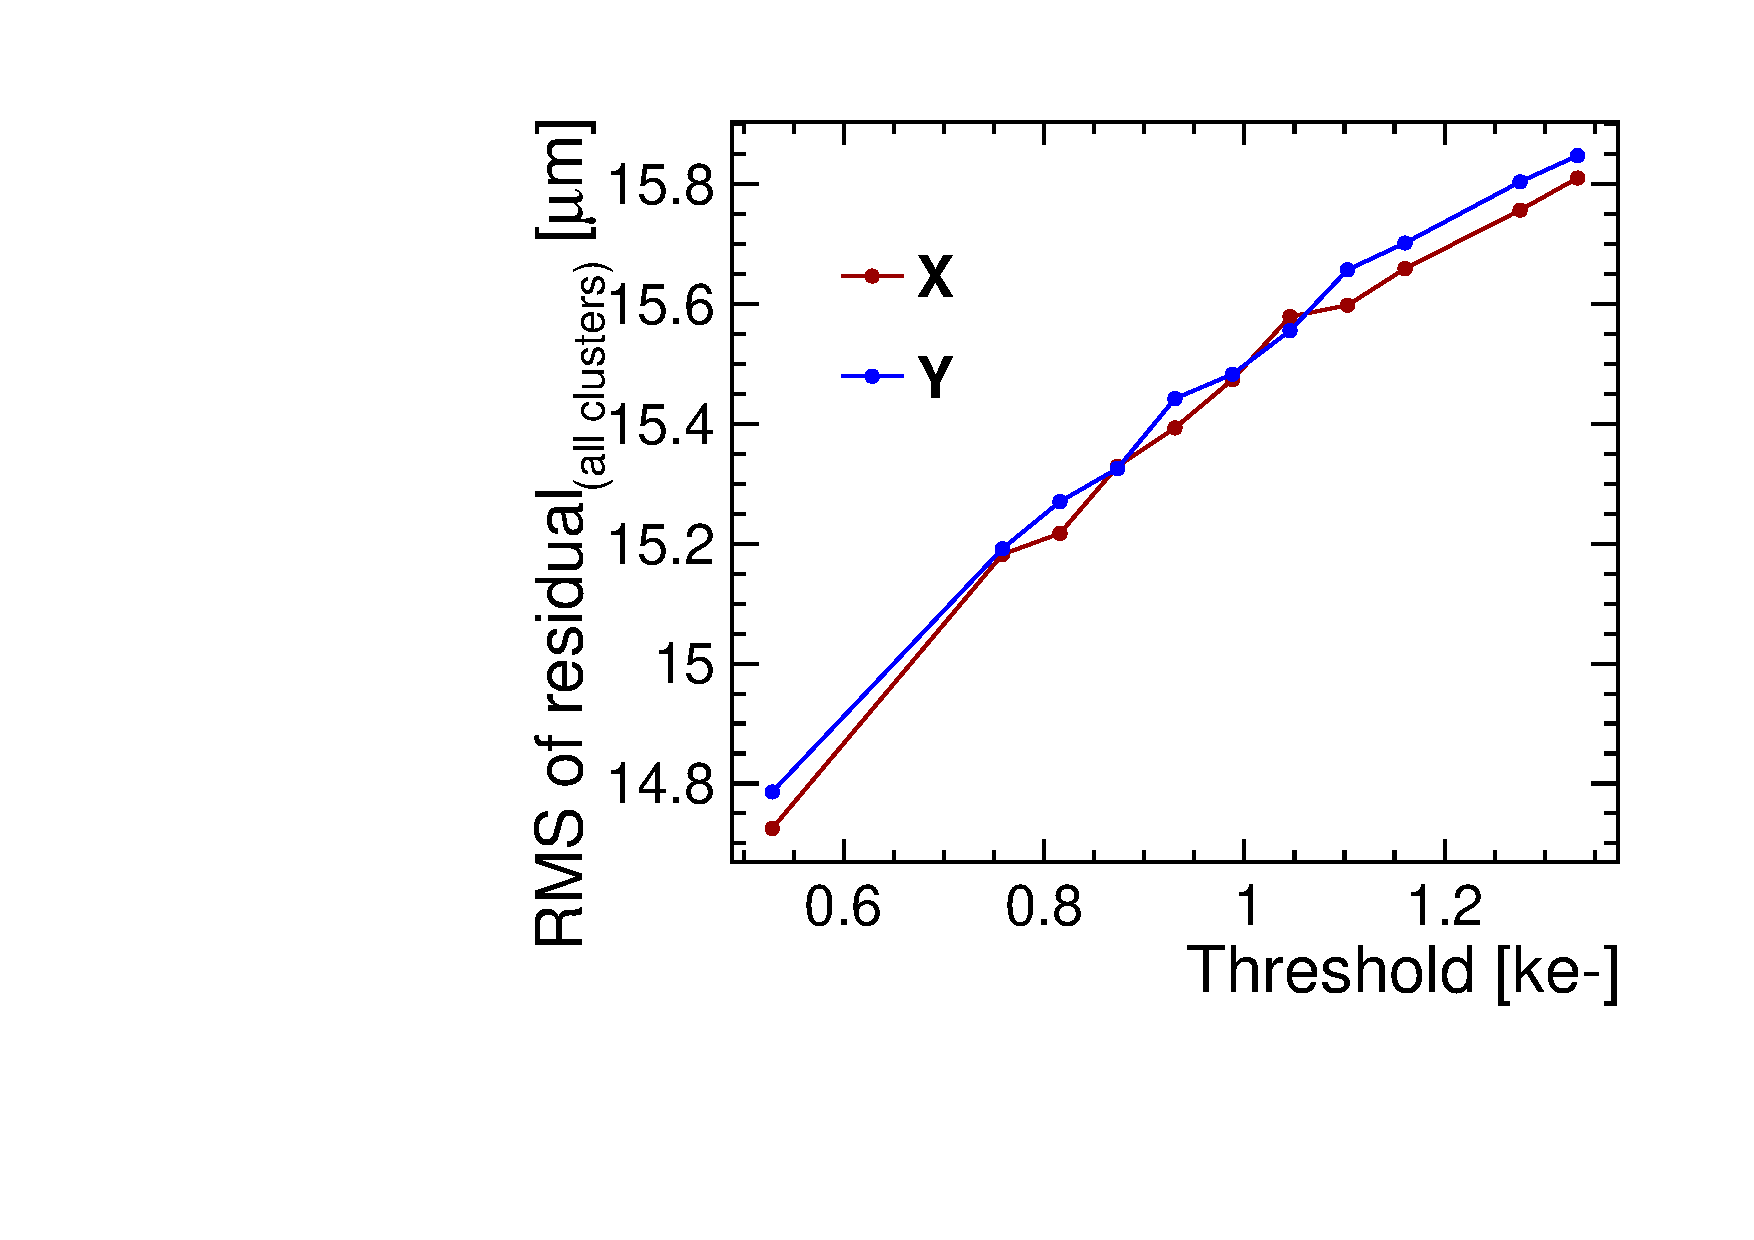
\includegraphics[width=\textwidth]{./figures/TestBeam/residuals_W0019_G07_THLscan.pdf}
    \caption{}
  \end{subfigure}
  \caption{The RMS of the residuals in x and y directions as a
    function of (a) bias voltage and (b) threshold for a $50\,\micron$
    thick sensor (assembly W19\_G7). The track resolution is not
    unfolded.}
  \label{fig:Residuals_bias_threshold}
\end{figure}


For the assemblies operated at the nominal operating conditions, the
RMS of the residuals in the x and y directions as a function of the
sensor thickness are shown in \cref{fig:residuals_thickness}. For
thicker sensors the fraction of multi-pixel clusters is higher and
results in lower residuals. The distribution of the residuals for
different sensor thicknesses operated at the nominal conditions is
shown in \cref{fig:residualsHist_thickness}. The wider component in
the residual distributions corresponds to the single-pixel
clusters. For thicker sensors, the fraction of multi-pixel clusters
increases. This leads to a higher fraction of more precisely
reconstructed hits and therefore the residual distribution gets
narrower.

\begin{figure}[htbp] 
  \centering
  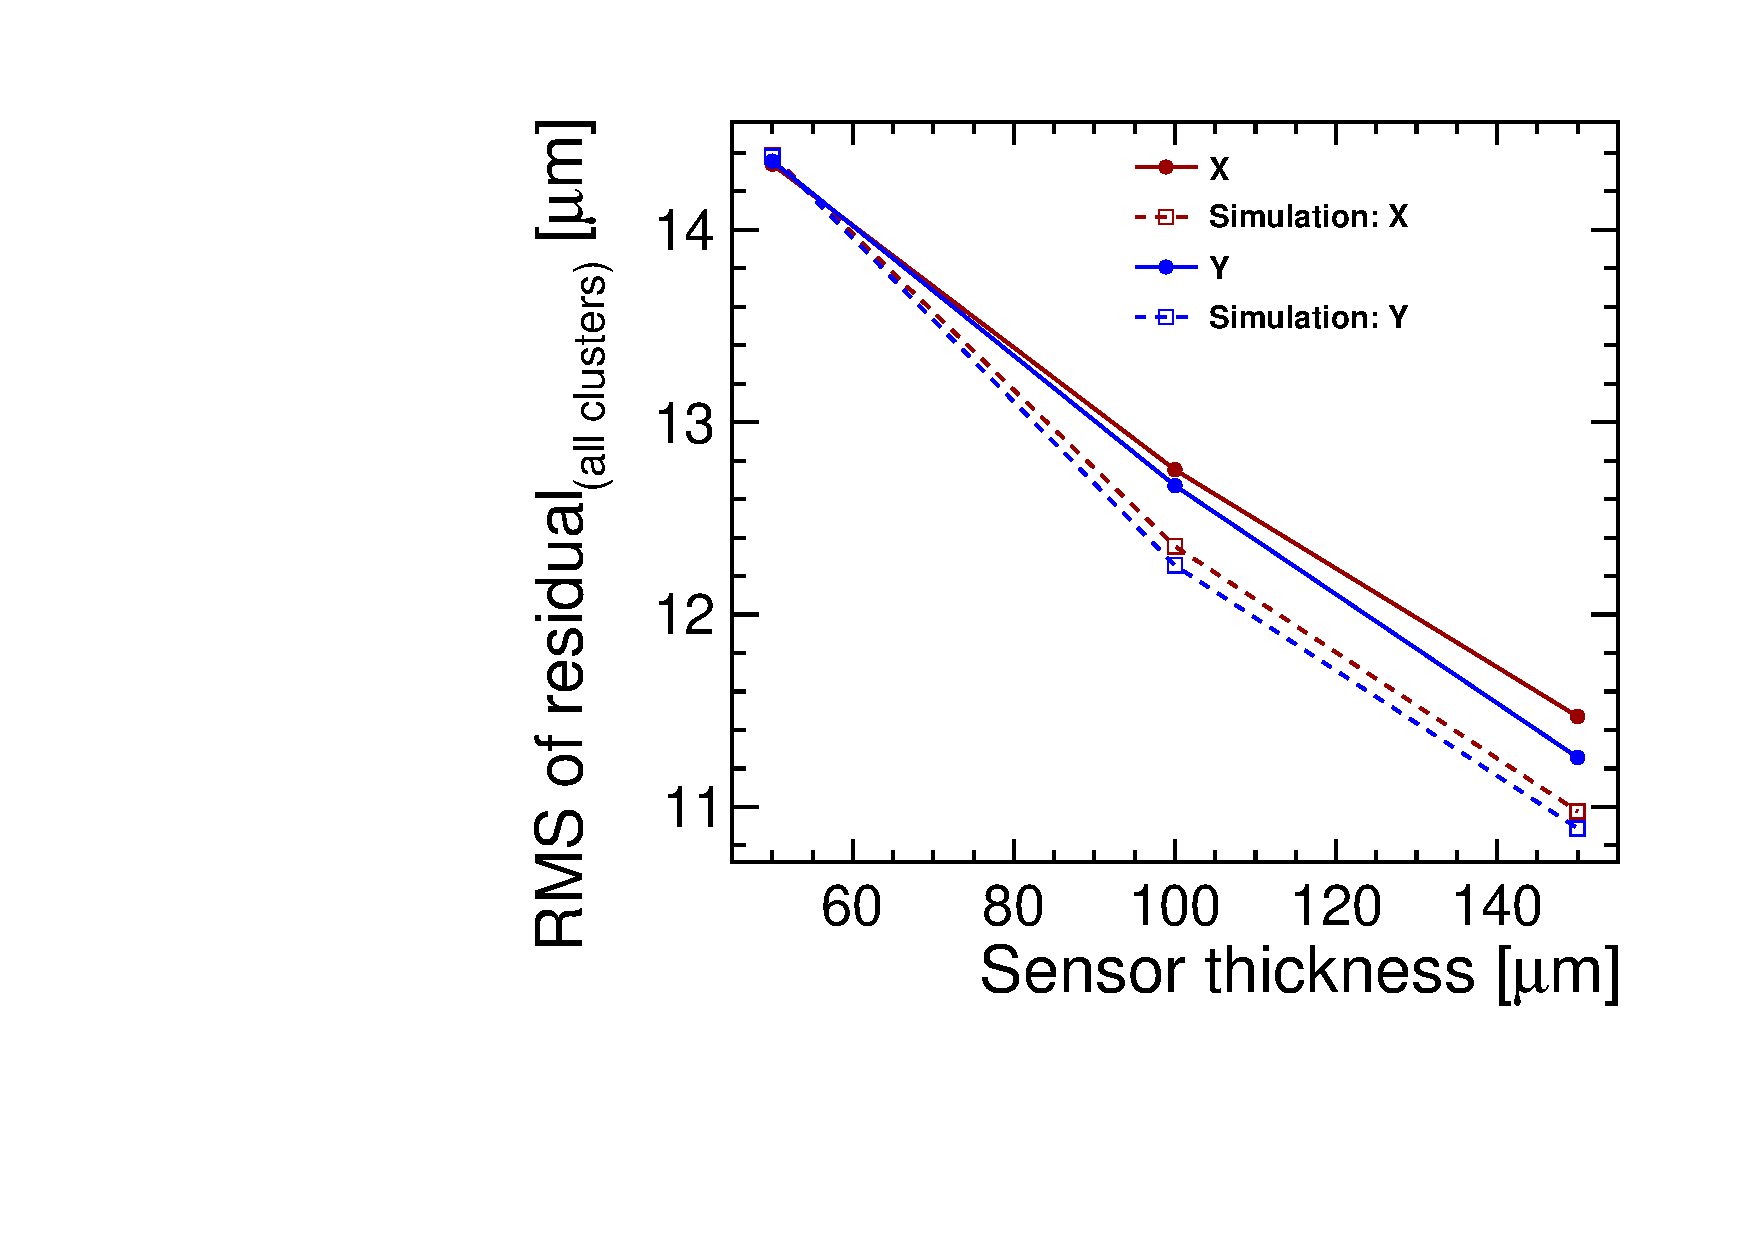
\includegraphics[width=0.5\textwidth]{./figures/TestBeam/residuals_vs_thickness.pdf}
  \caption{The RMS of the residuals in x and y directions as a
    function of the sensor thickness for assemblies operated at the
    nominal condition. The track resolution is not unfolded.}
  \label{fig:residuals_thickness}
\end{figure}


\begin{figure}[htbp] \centering
  \begin{subfigure}[b]{0.23\textwidth}
    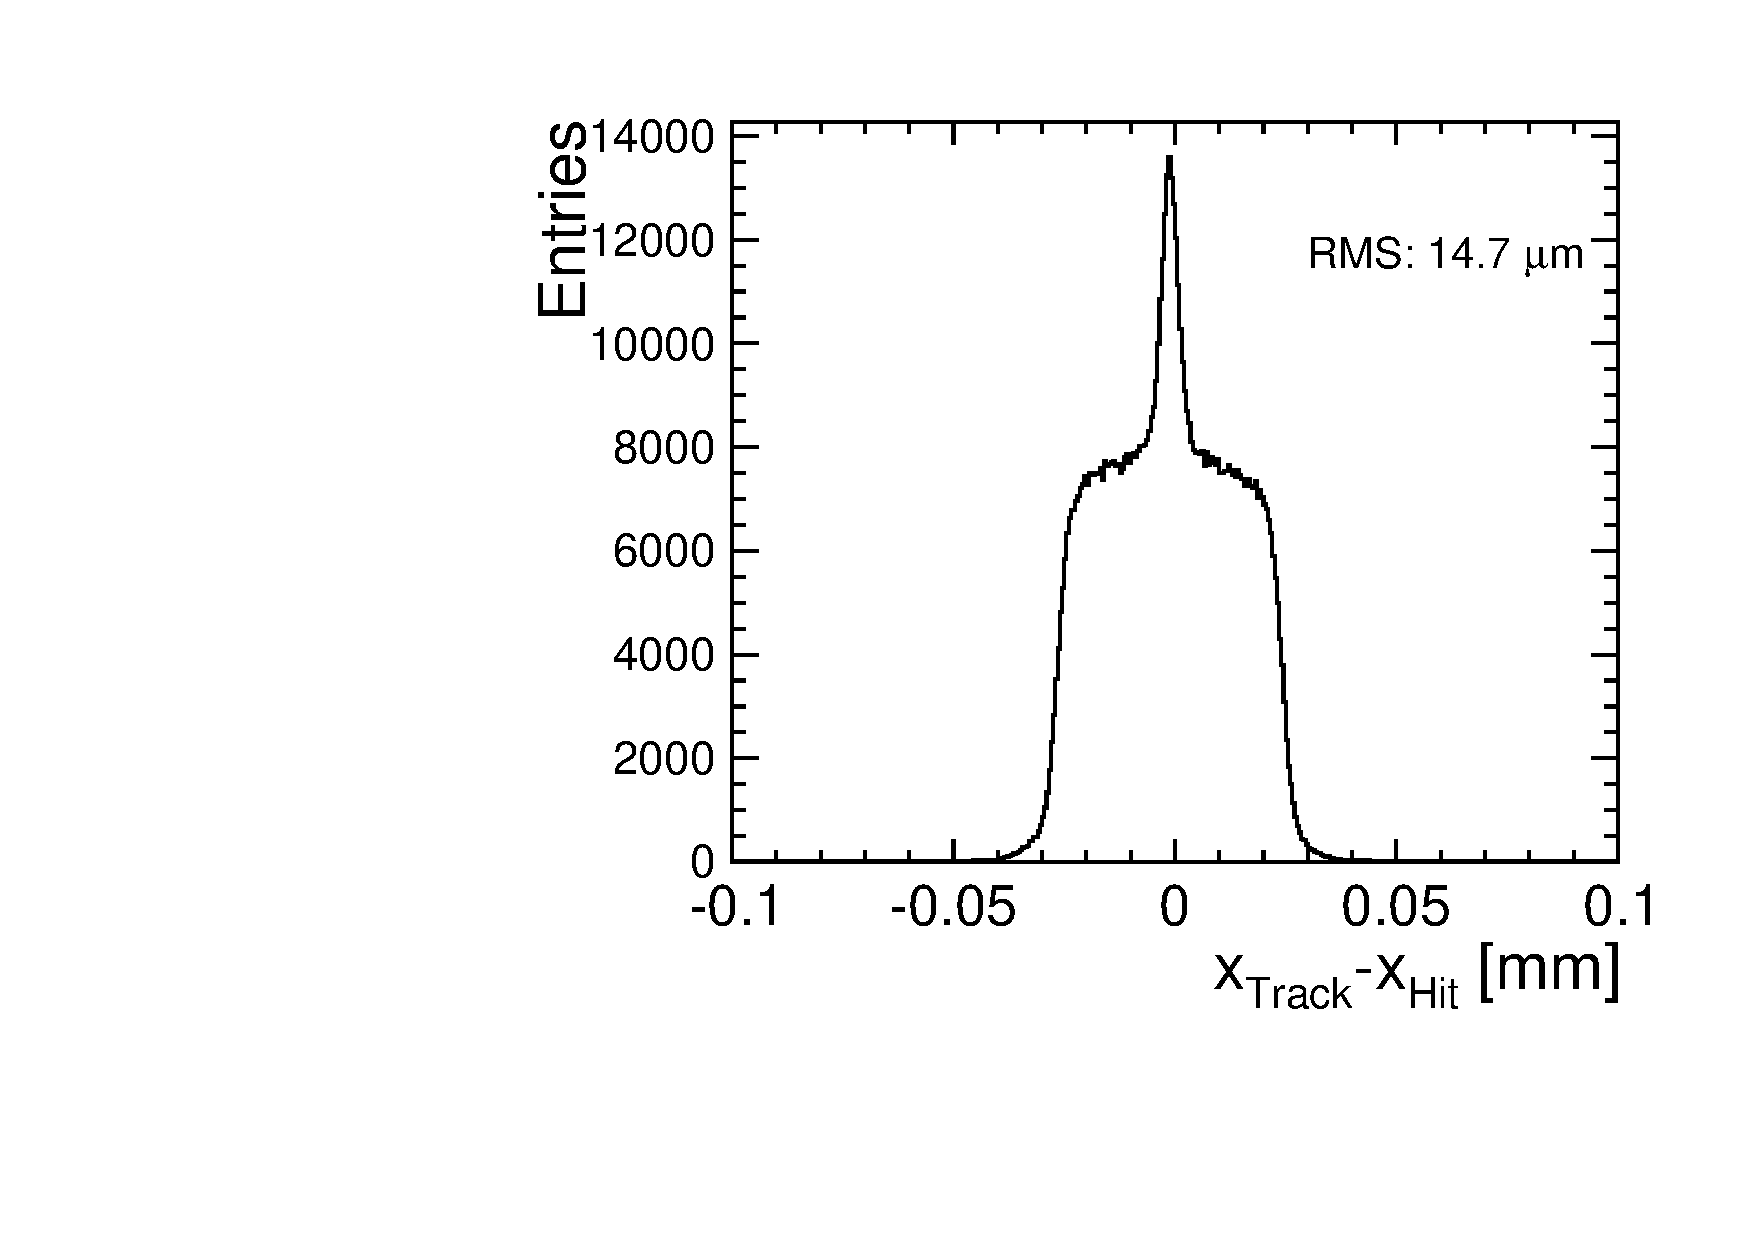
\includegraphics[width=\textwidth]{./figures/TestBeam/residualsHist_W19_C7.pdf}
    \caption{$50\,\micron$ sensor}
  \end{subfigure} \hfill
  \begin{subfigure}[b]{0.23\textwidth}
    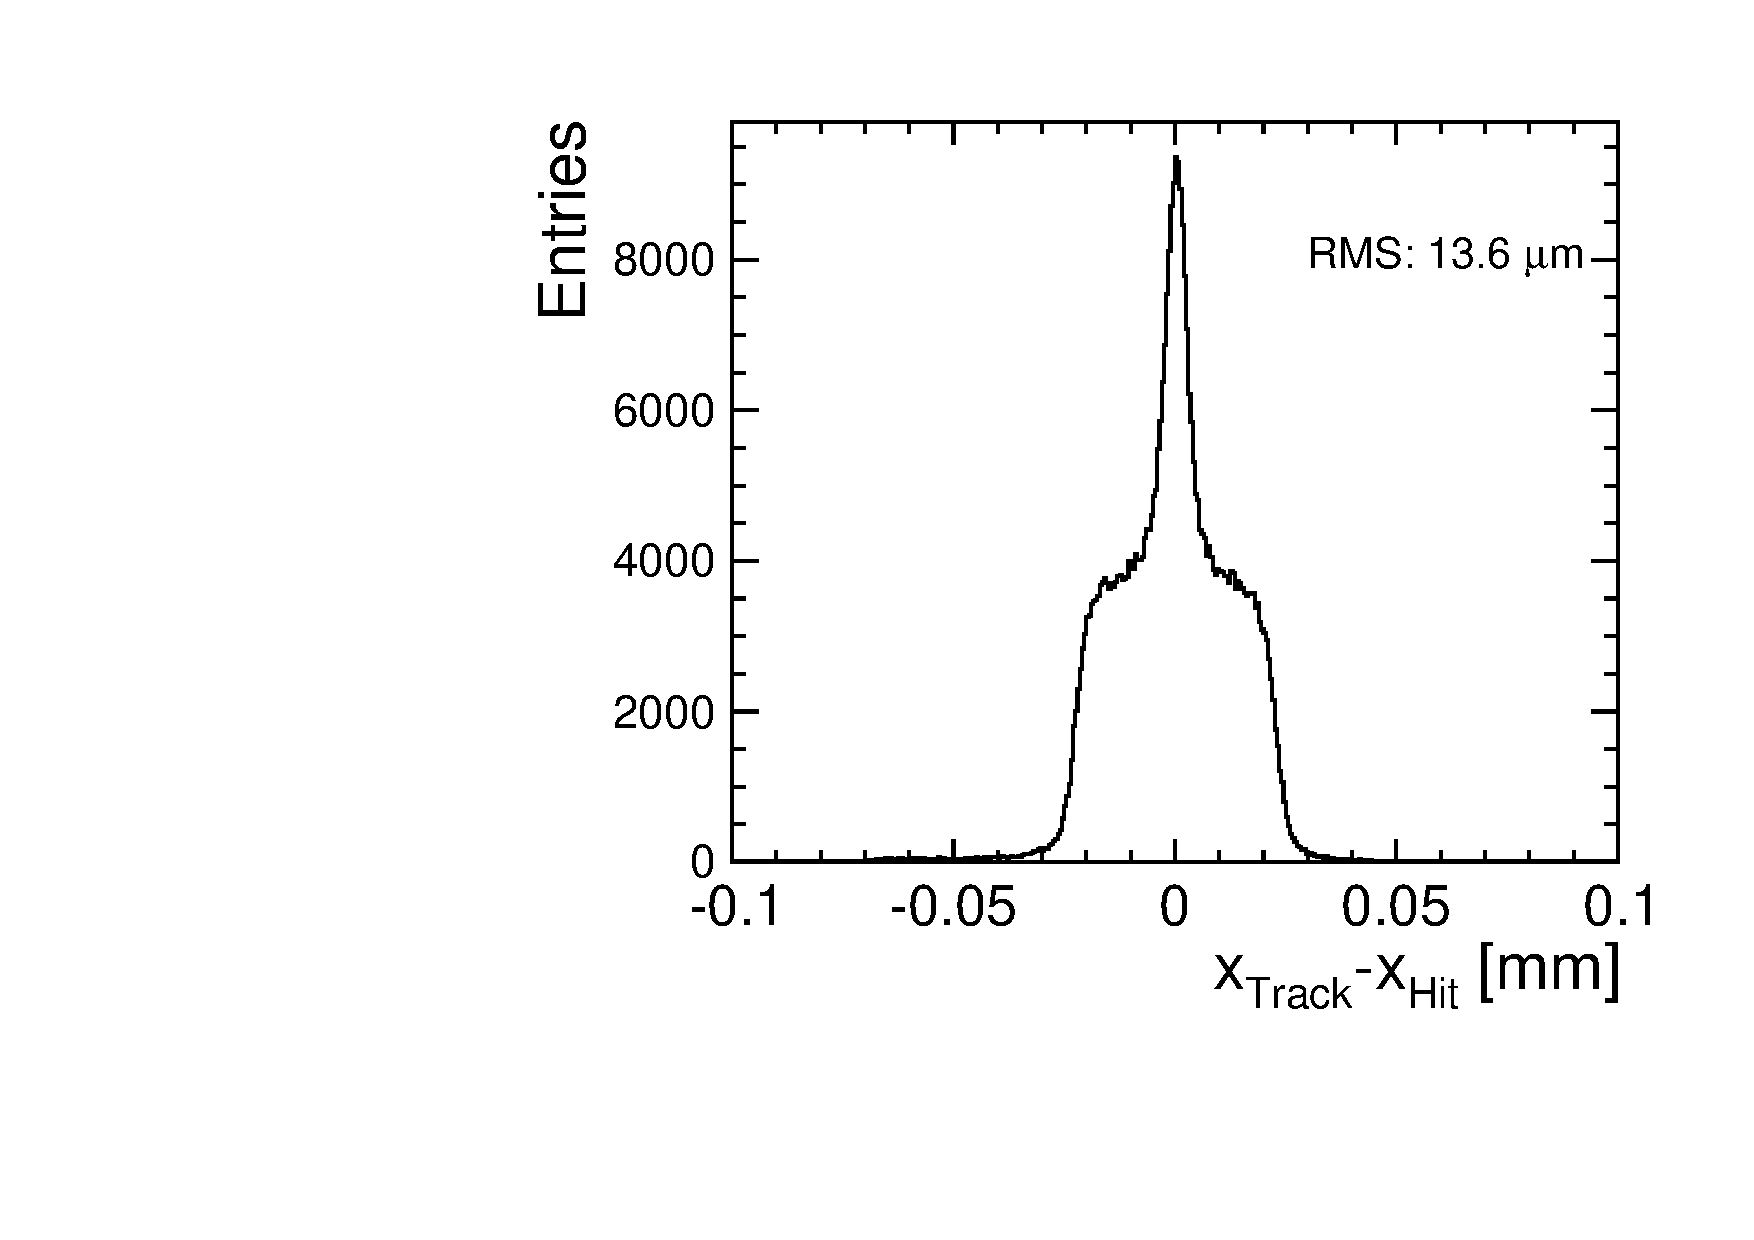
\includegraphics[width=\textwidth]{./figures/TestBeam/residualsHist_W5_E2.pdf}
    \caption{$100\,\micron$ sensor}
  \end{subfigure} \hfill
  \begin{subfigure}[b]{0.23\textwidth}
    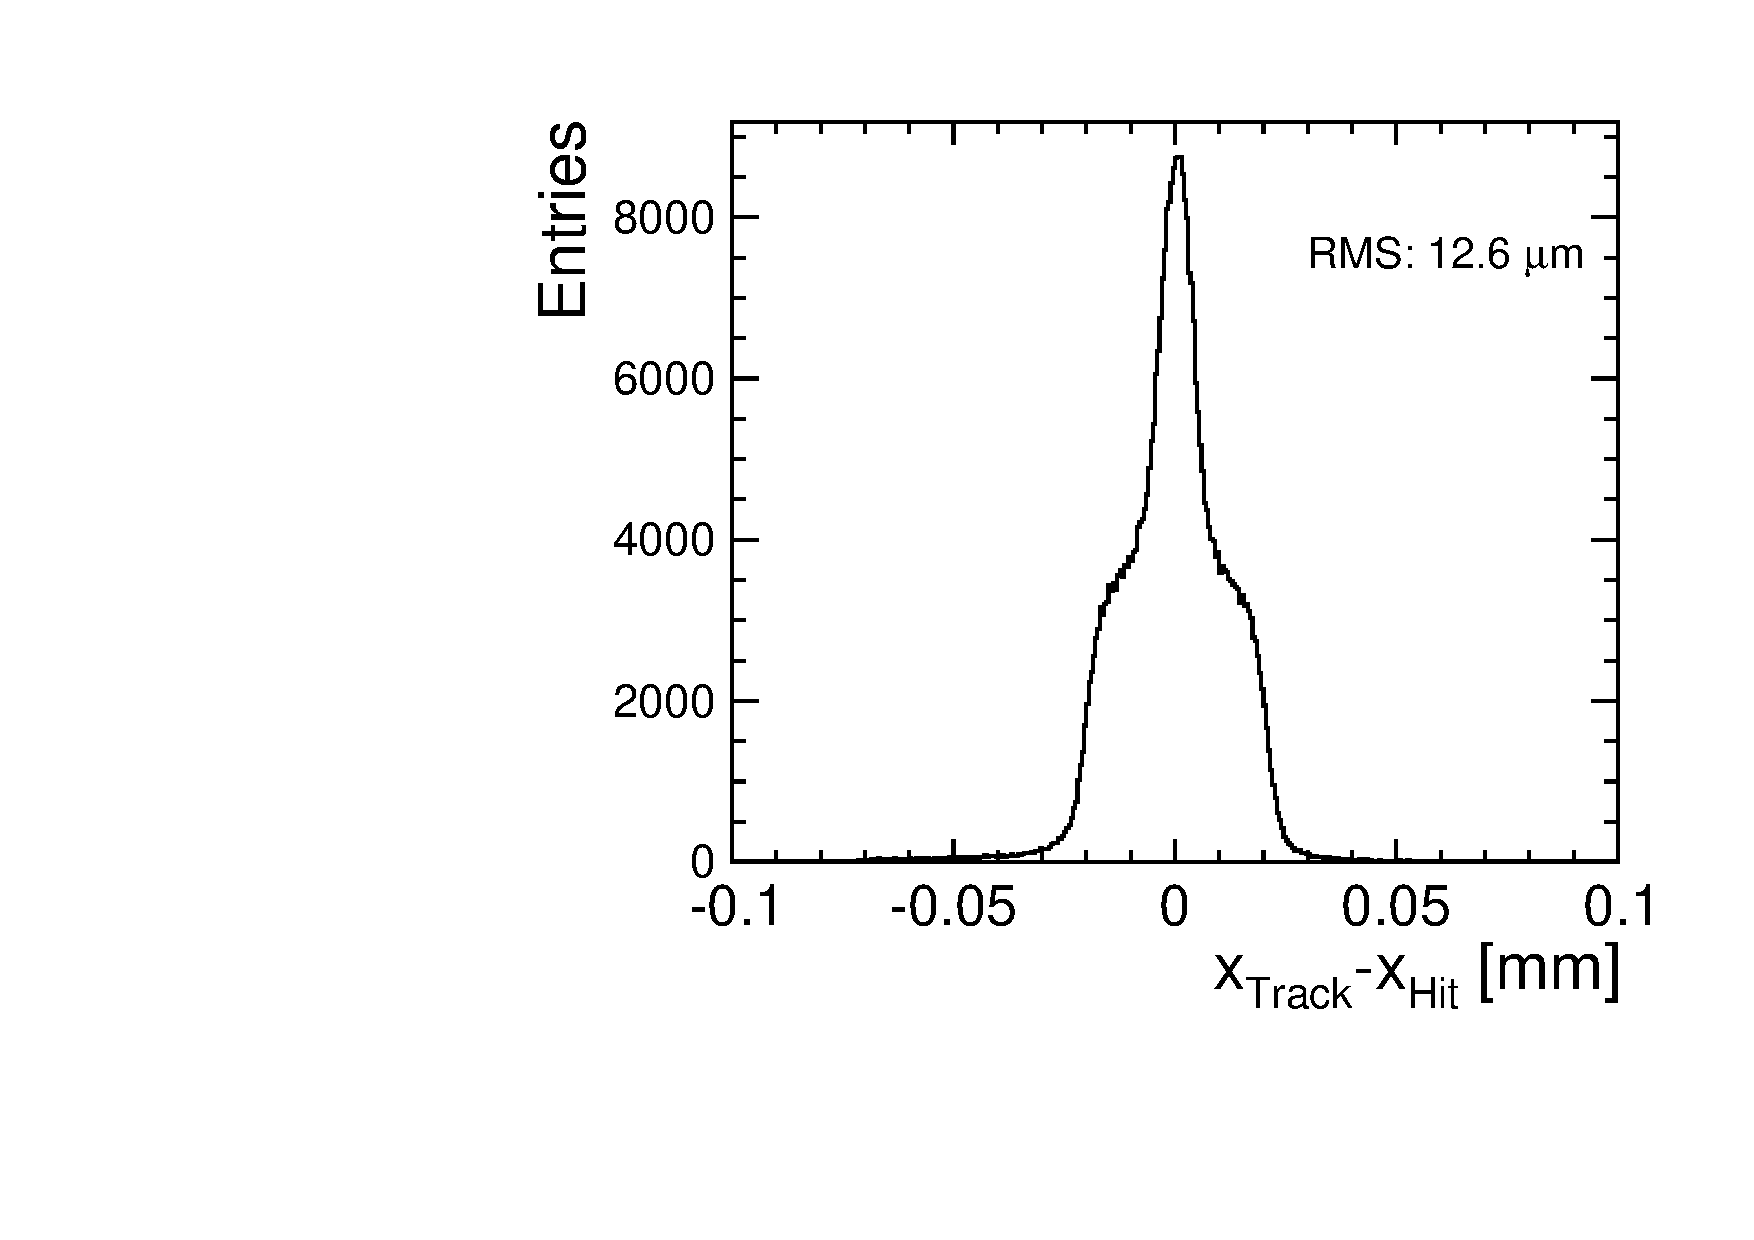
\includegraphics[width=\textwidth]{./figures/TestBeam/residualsHist_W5_F1.pdf}
    \caption{$150\,\micron$ sensor}
  \end{subfigure} \hfill
  \begin{subfigure}[b]{0.23\textwidth}

    \caption{$300\,\micron$ sensor}
  \end{subfigure}
  \caption{Examples of the residuals distributions in the x direction
    for the assemblies (a) W19\_C7, (b) W5\_E2 and (c) W5\_F1. The
    track resolution is not unfolded.}
  \label{fig:residualsHist_thickness}
\end{figure}
%% --------------------------------------------- %%
\subsection{Global detection efficiency}

The detection efficiency of the assemblies is defined as the fraction
of total number of hits matched to tracks (within a window of radius
0.1~mm) and the total number of tracks projected to pass through the
assembly. The efficiency is calculated within the matrix of
$256\times256$ pixels of the main sensor area and the hot or masked
pixels are not excluded from this calculation. They contribute to the
assemblies' inefficiencies.

The detection efficiency is strongly related to the operating
threshold of the readout ASIC. With a lower threshold, smaller energy
depositions can be measured and it is more likely to detect a
track. \cref{fig:efficiency_VS_Threshold} shows the detection
efficiency for different sensor thicknesses. For thinner sensors, the
energy deposition is lower and the efficiency drops more quickly by
increasing the threshold than for thick sensors.

\begin{figure}[htbp] 
  \centering
  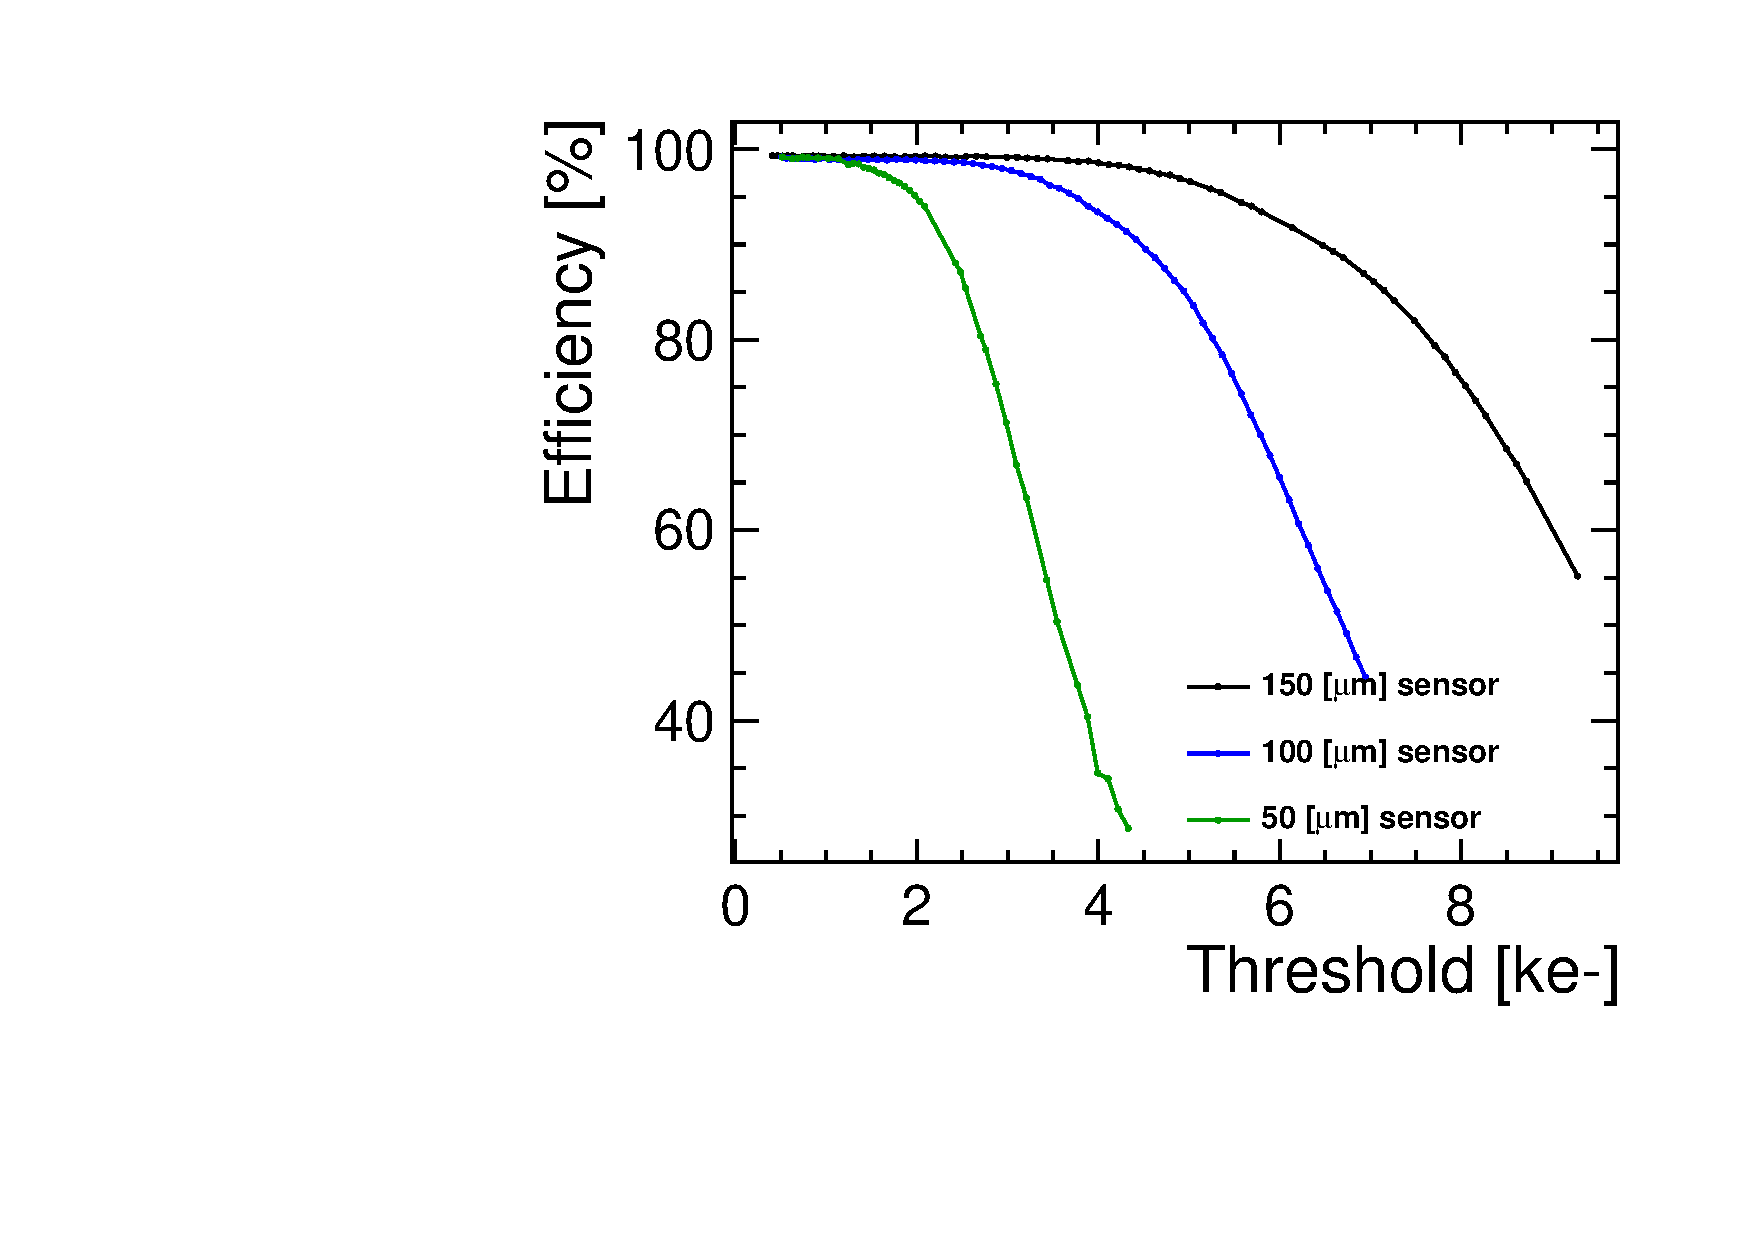
\includegraphics[width=0.5\textwidth]{./figures/TestBeam/Efficiency_vs_THL.pdf}
  \caption{Global detection efficiency as a function of the threshold
    of the readout ASIC for different sensor thicknesses.}
  \label{fig:efficiency_VS_Threshold}
\end{figure}



%% --------------------------------------------- %%
\section{Calibrated test beam data}

The test pulse calibration as described in
\cref{sec:EnergyCalibration} is applied to the test beam data in order
to convert the TOT values into energy deposited (in electrons) by the
MIP particles.


\cref{sec:testBeamDataCalibrated_TOT} shows the TOT distribution for
one, two, three and four-hit clusters. The MPV of the TOT
distributions for different cluster sizes do not align due to the
non-linear behaviour of the Timepix3, as sharing the same deposited
charge amongst several pixels results in each pixel having a higher
TOT than would be expected from simply scaling the charge. The
calibrated energy distribution aligns for different cluster sizes
since the calibration takes into account the non-linearities of the
chip as shown in \cref{sec:testBeamDataCalibrated_Edep}. For the
$50\,\micron$ thick sensor, the calibrated distributions do not
align. This is due to the low energy deposition in thin sensors
especially for multi-hit clusters where the energy deposition per
pixel is close to the threshold.

\begin{figure}[htbp] \centering
  \begin{subfigure}[b]{0.33\textwidth}
    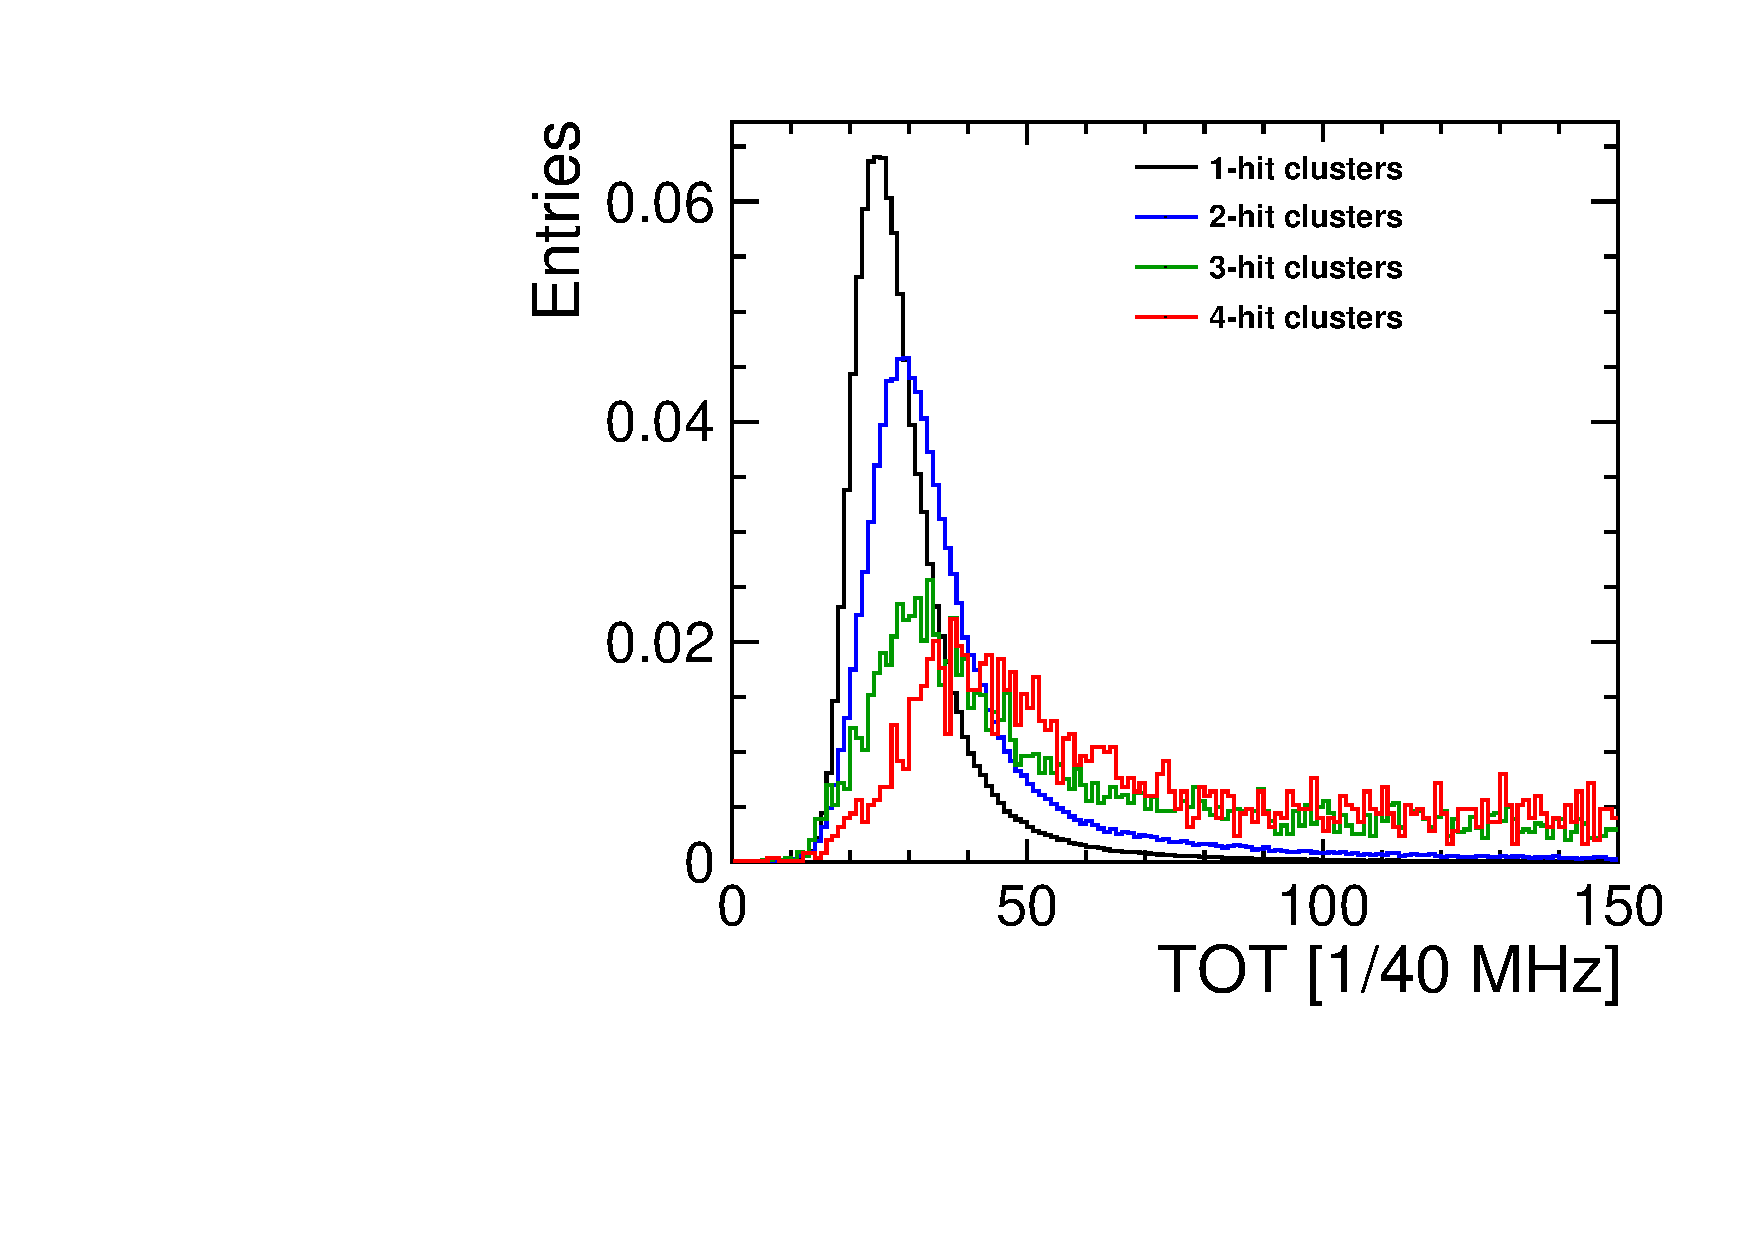
\includegraphics[width=\textwidth]{./figures/Calibration/TOT_Clusters_W0019_C07.pdf}
    \caption{W19\_C7}
  \end{subfigure} \hfill
  \begin{subfigure}[b]{0.33\textwidth}
    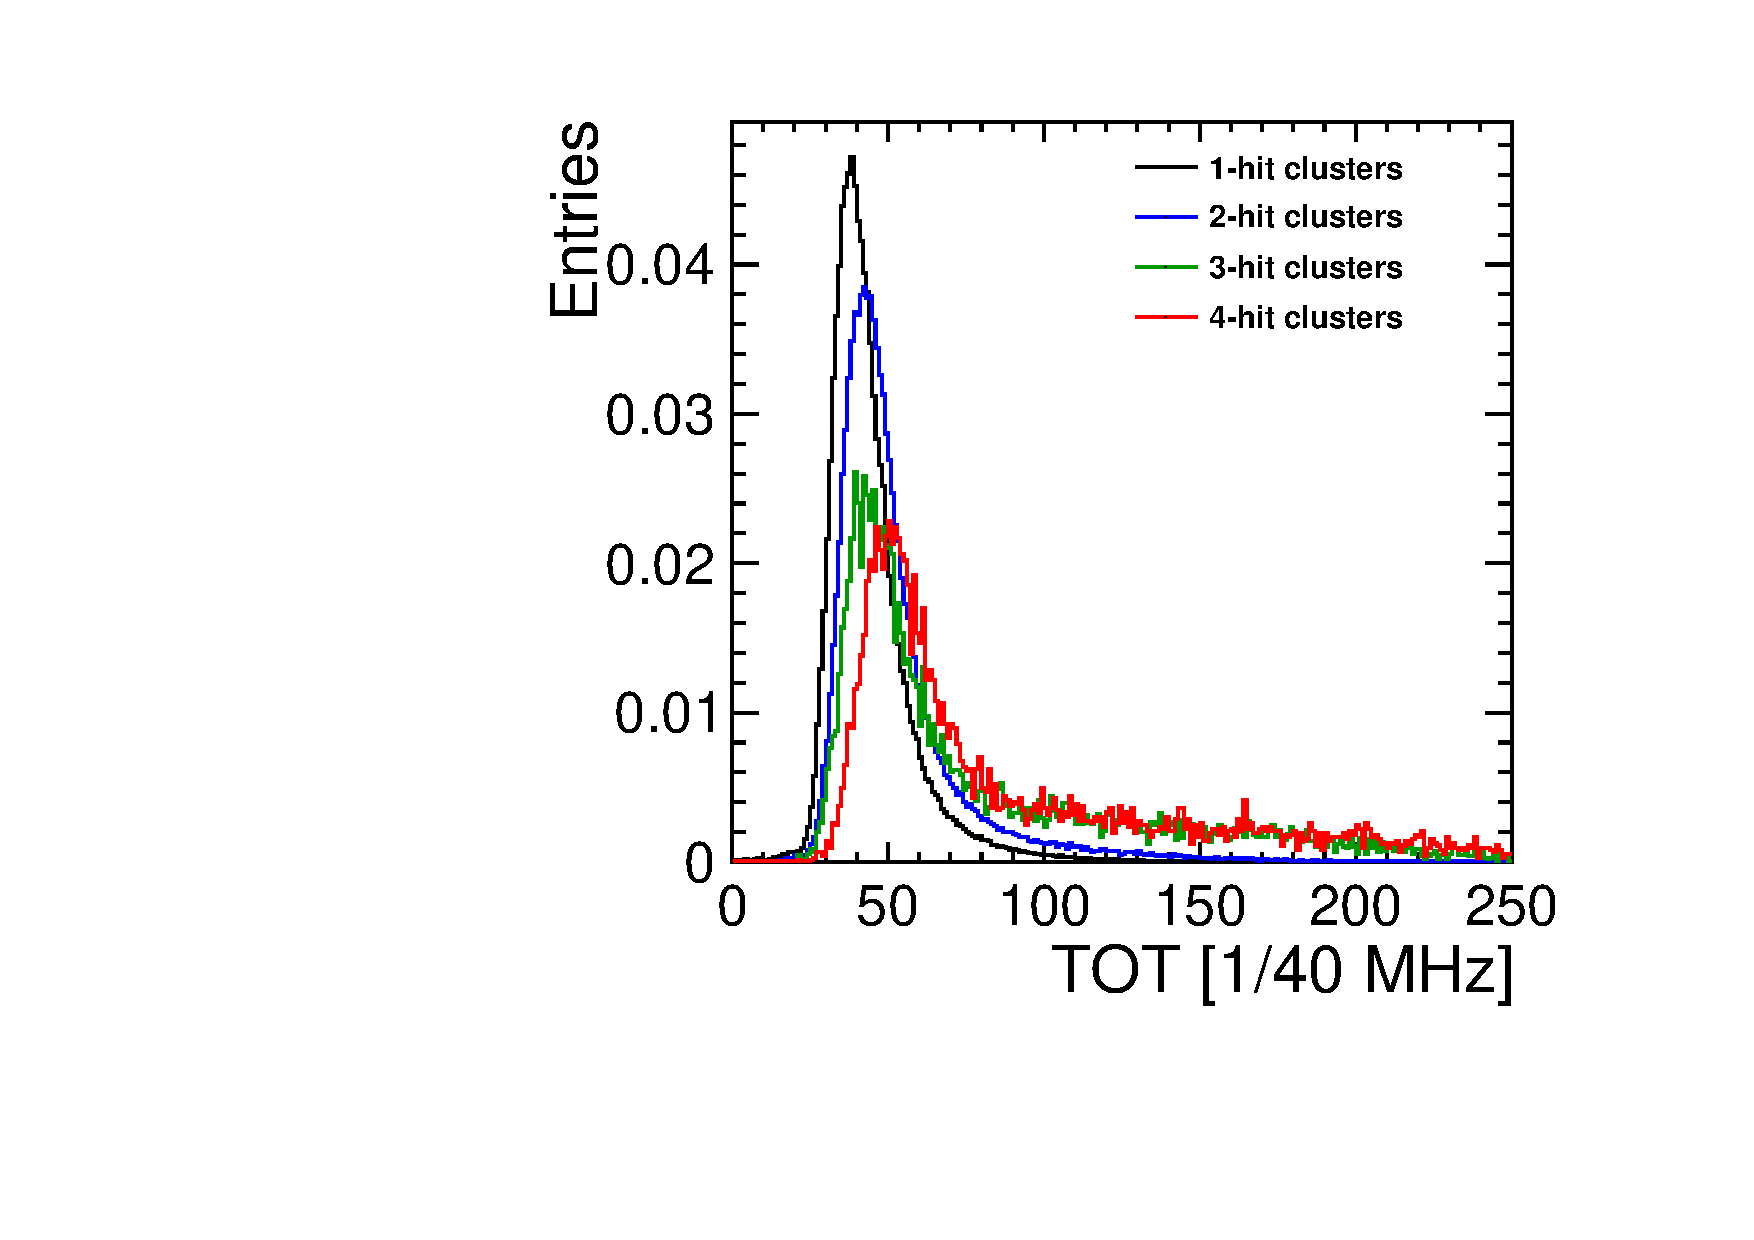
\includegraphics[width=\textwidth]{./figures/Calibration/TOT_Clusters_W0005_E02.pdf}
    \caption{W5\_E2}
  \end{subfigure}\hfill
  \begin{subfigure}[b]{0.33\textwidth}
    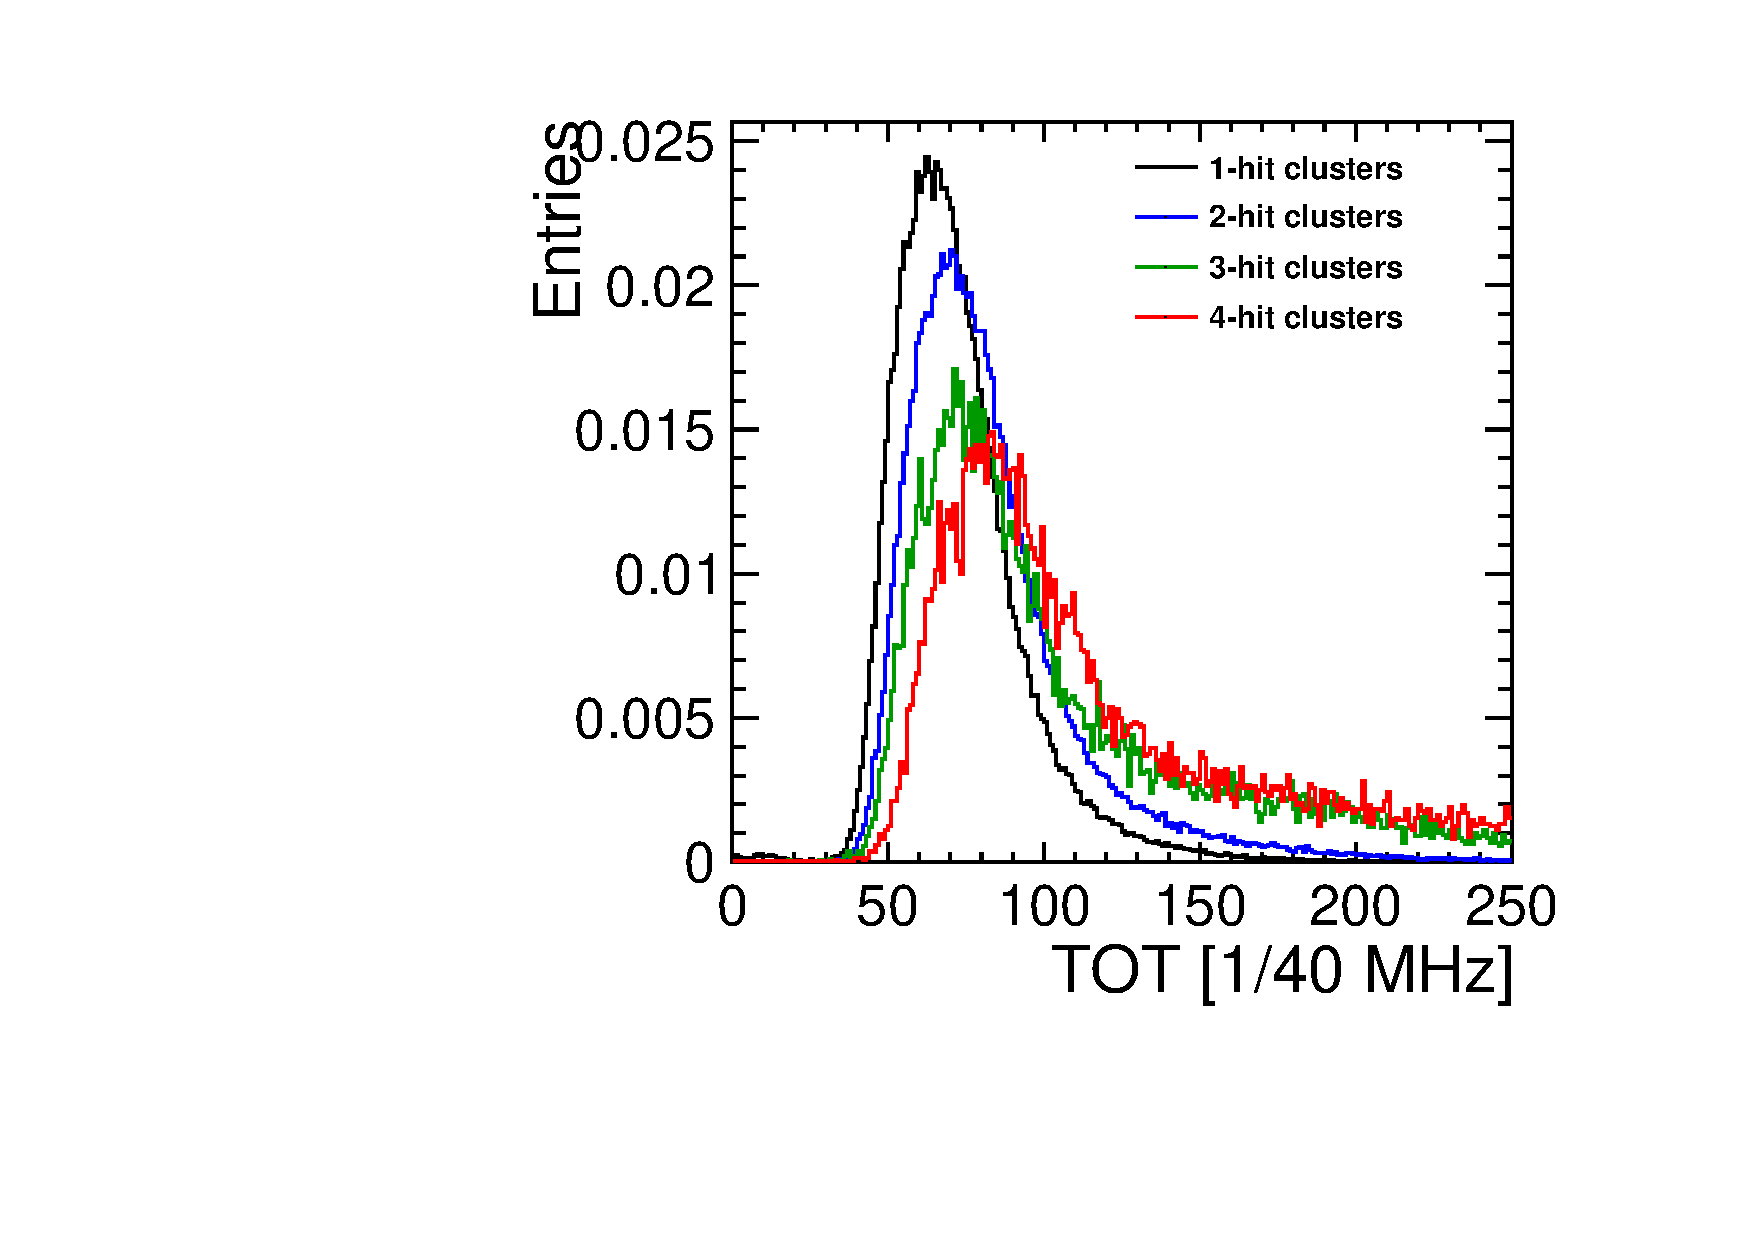
\includegraphics[width=\textwidth]{./figures/Calibration/TOT_Clusters_W0005_F01.pdf}
    \caption{W5\_F1}
  \end{subfigure}
  \caption{TOT distribution for one, two, three and four-hit clusters
    for various assemblies with (a) $50\,\micron$, (b) $100\,\micron$
    and (c) $150\,\micron$ thick planar sensors.}
  \label{sec:testBeamDataCalibrated_TOT}
\end{figure}

\begin{figure}[htbp] \centering
  \begin{subfigure}[b]{0.33\textwidth}
    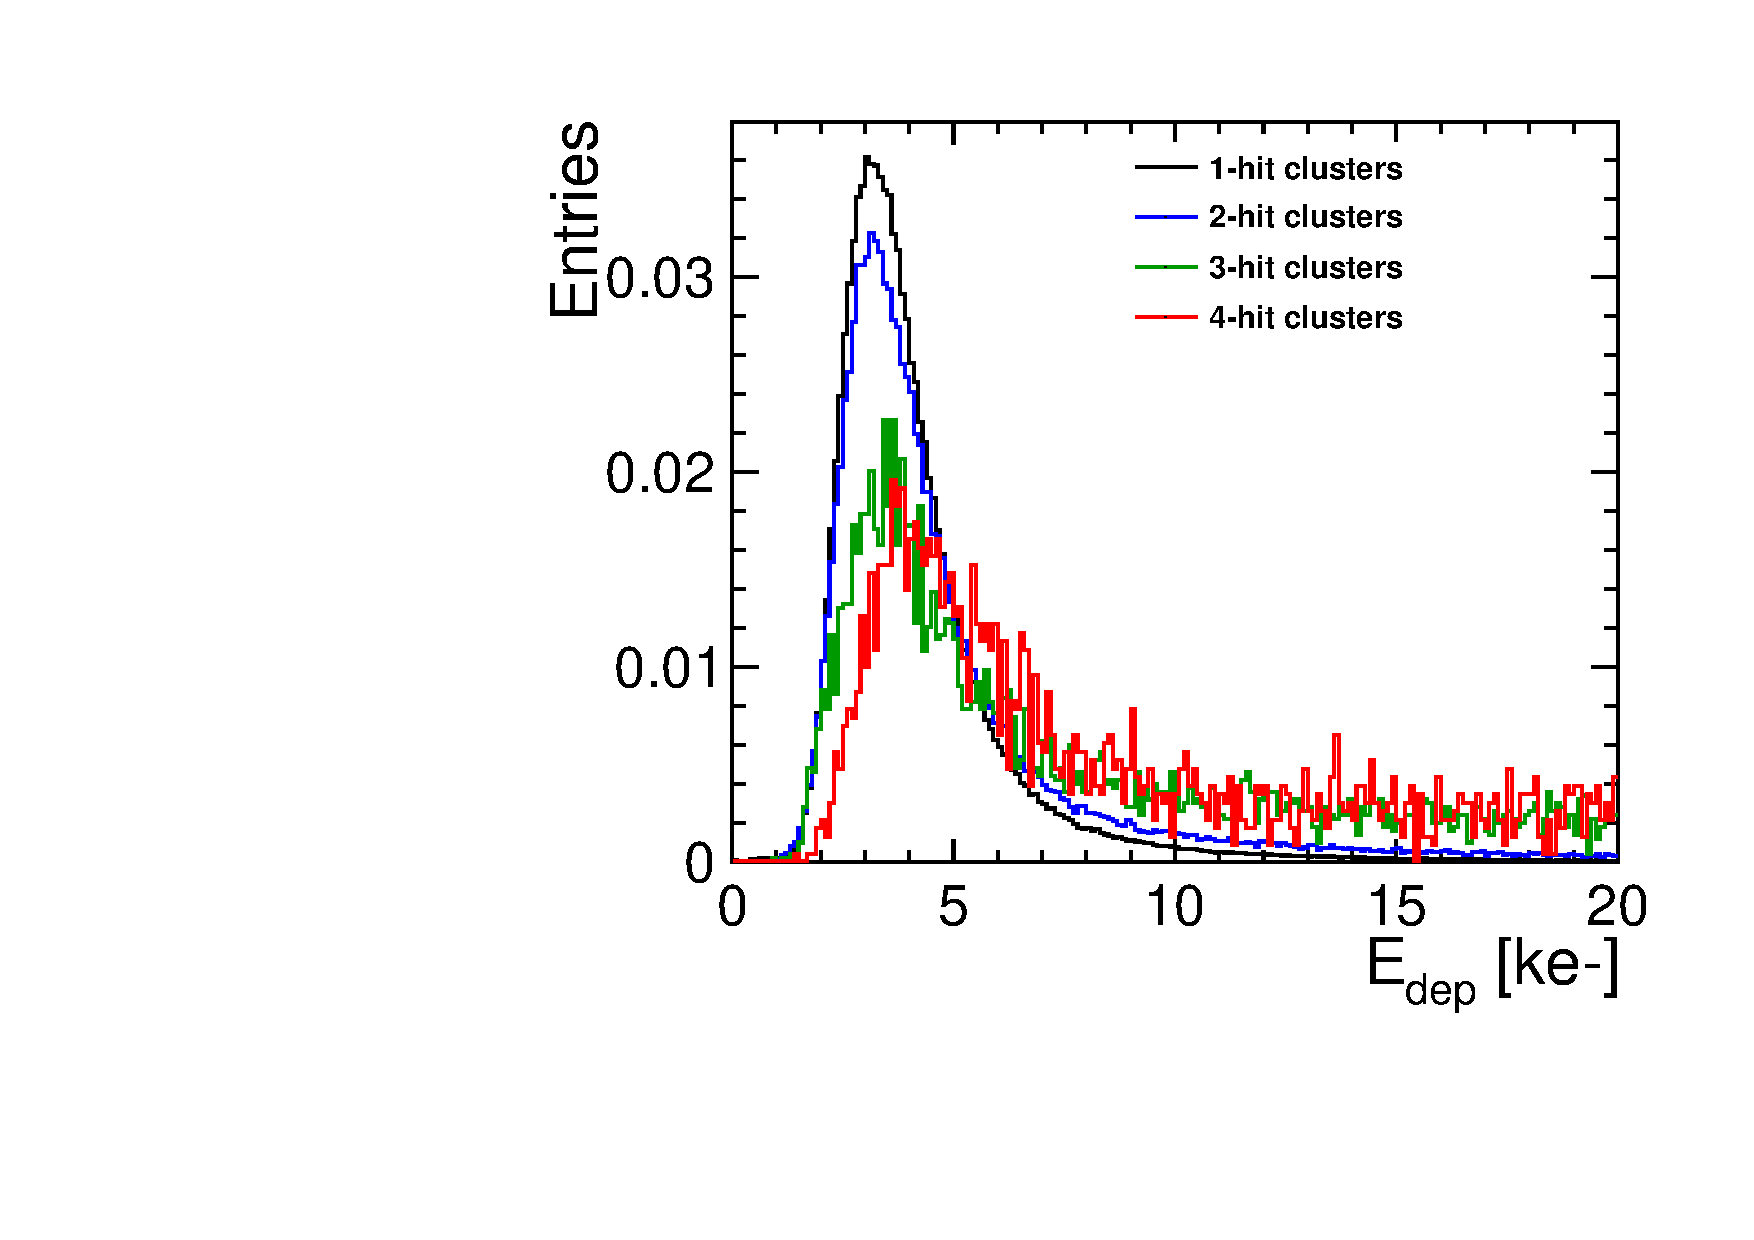
\includegraphics[width=\textwidth]{./figures/Calibration/Edep_Clusters_W0019_C07.pdf}
    \caption{W19\_C7}
  \end{subfigure} \hfill
  \begin{subfigure}[b]{0.33\textwidth}
    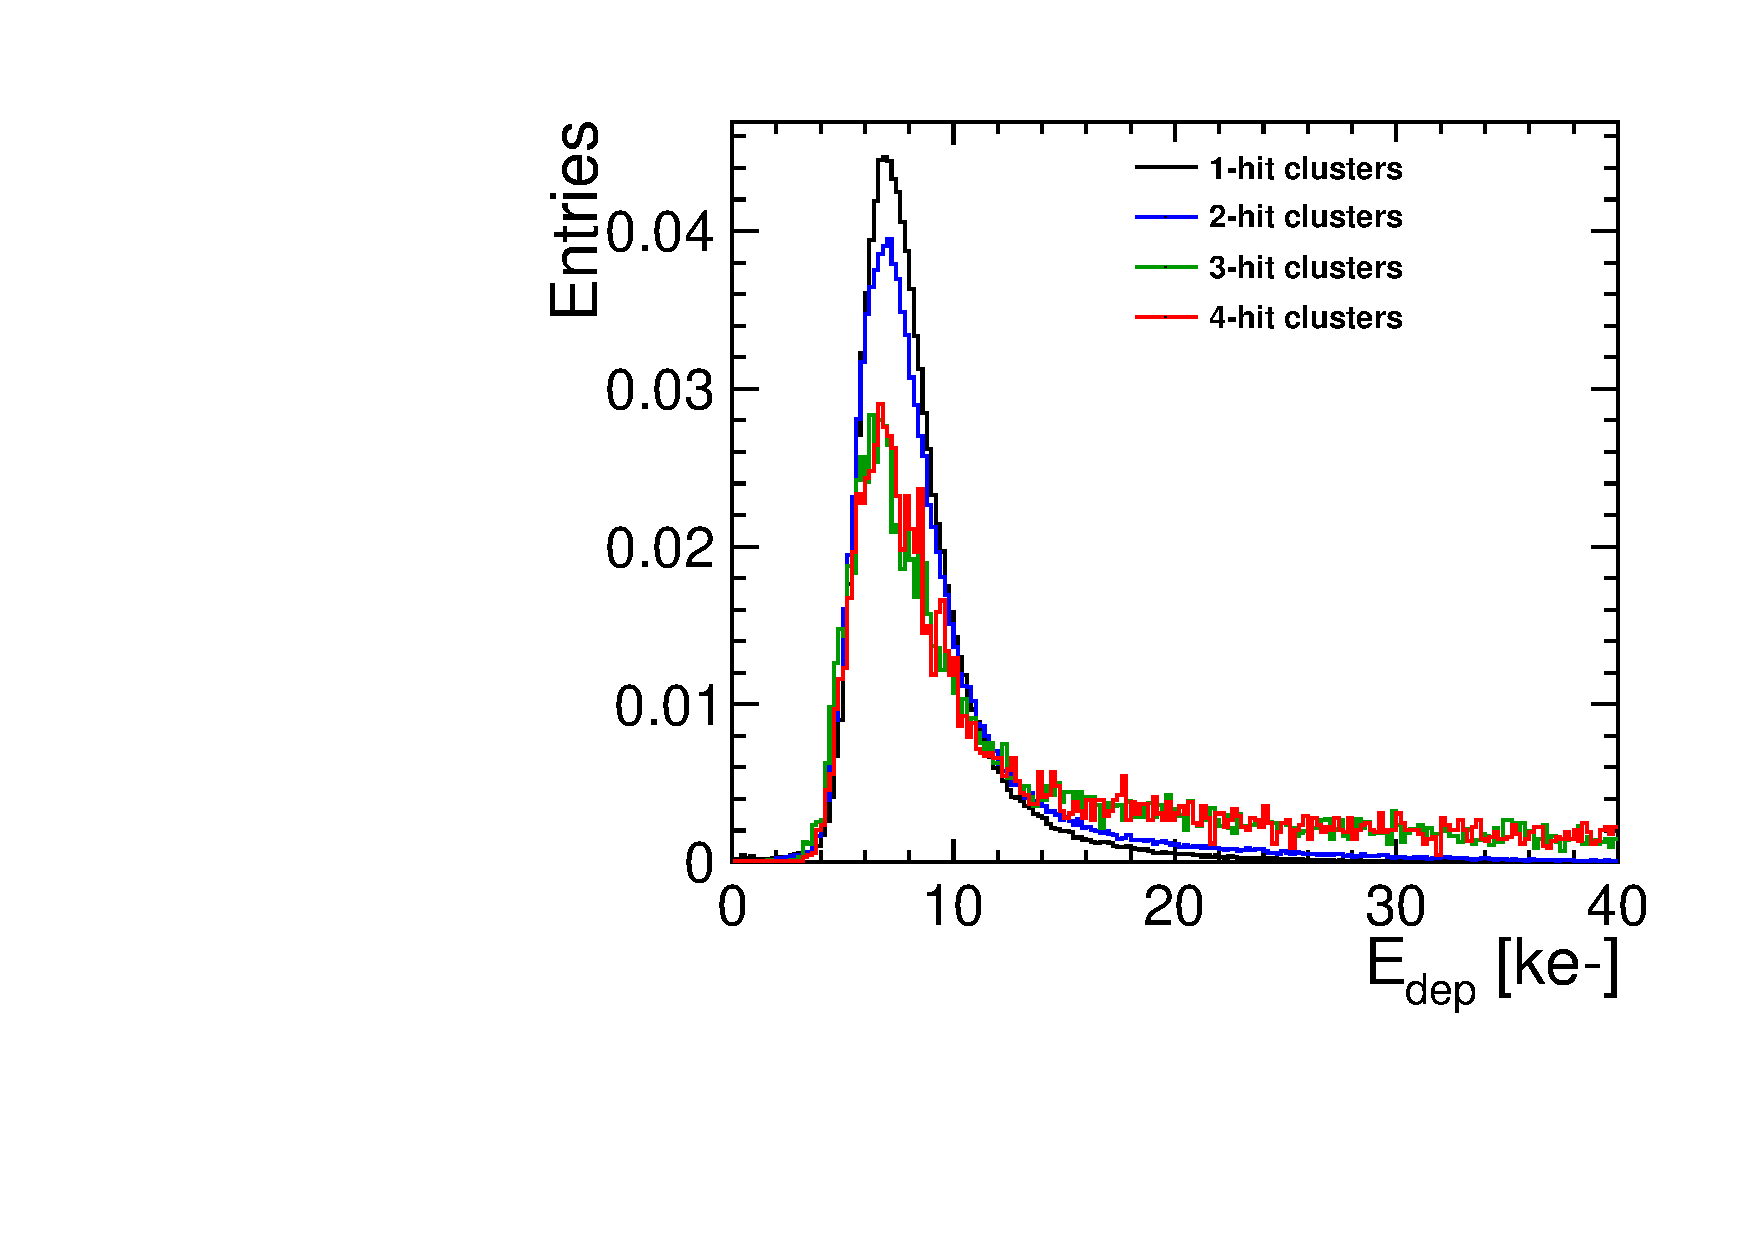
\includegraphics[width=\textwidth]{./figures/Calibration/Edep_Clusters_W0005_E02.pdf}
    \caption{W5\_E2}
  \end{subfigure}\hfill
  \begin{subfigure}[b]{0.33\textwidth}
    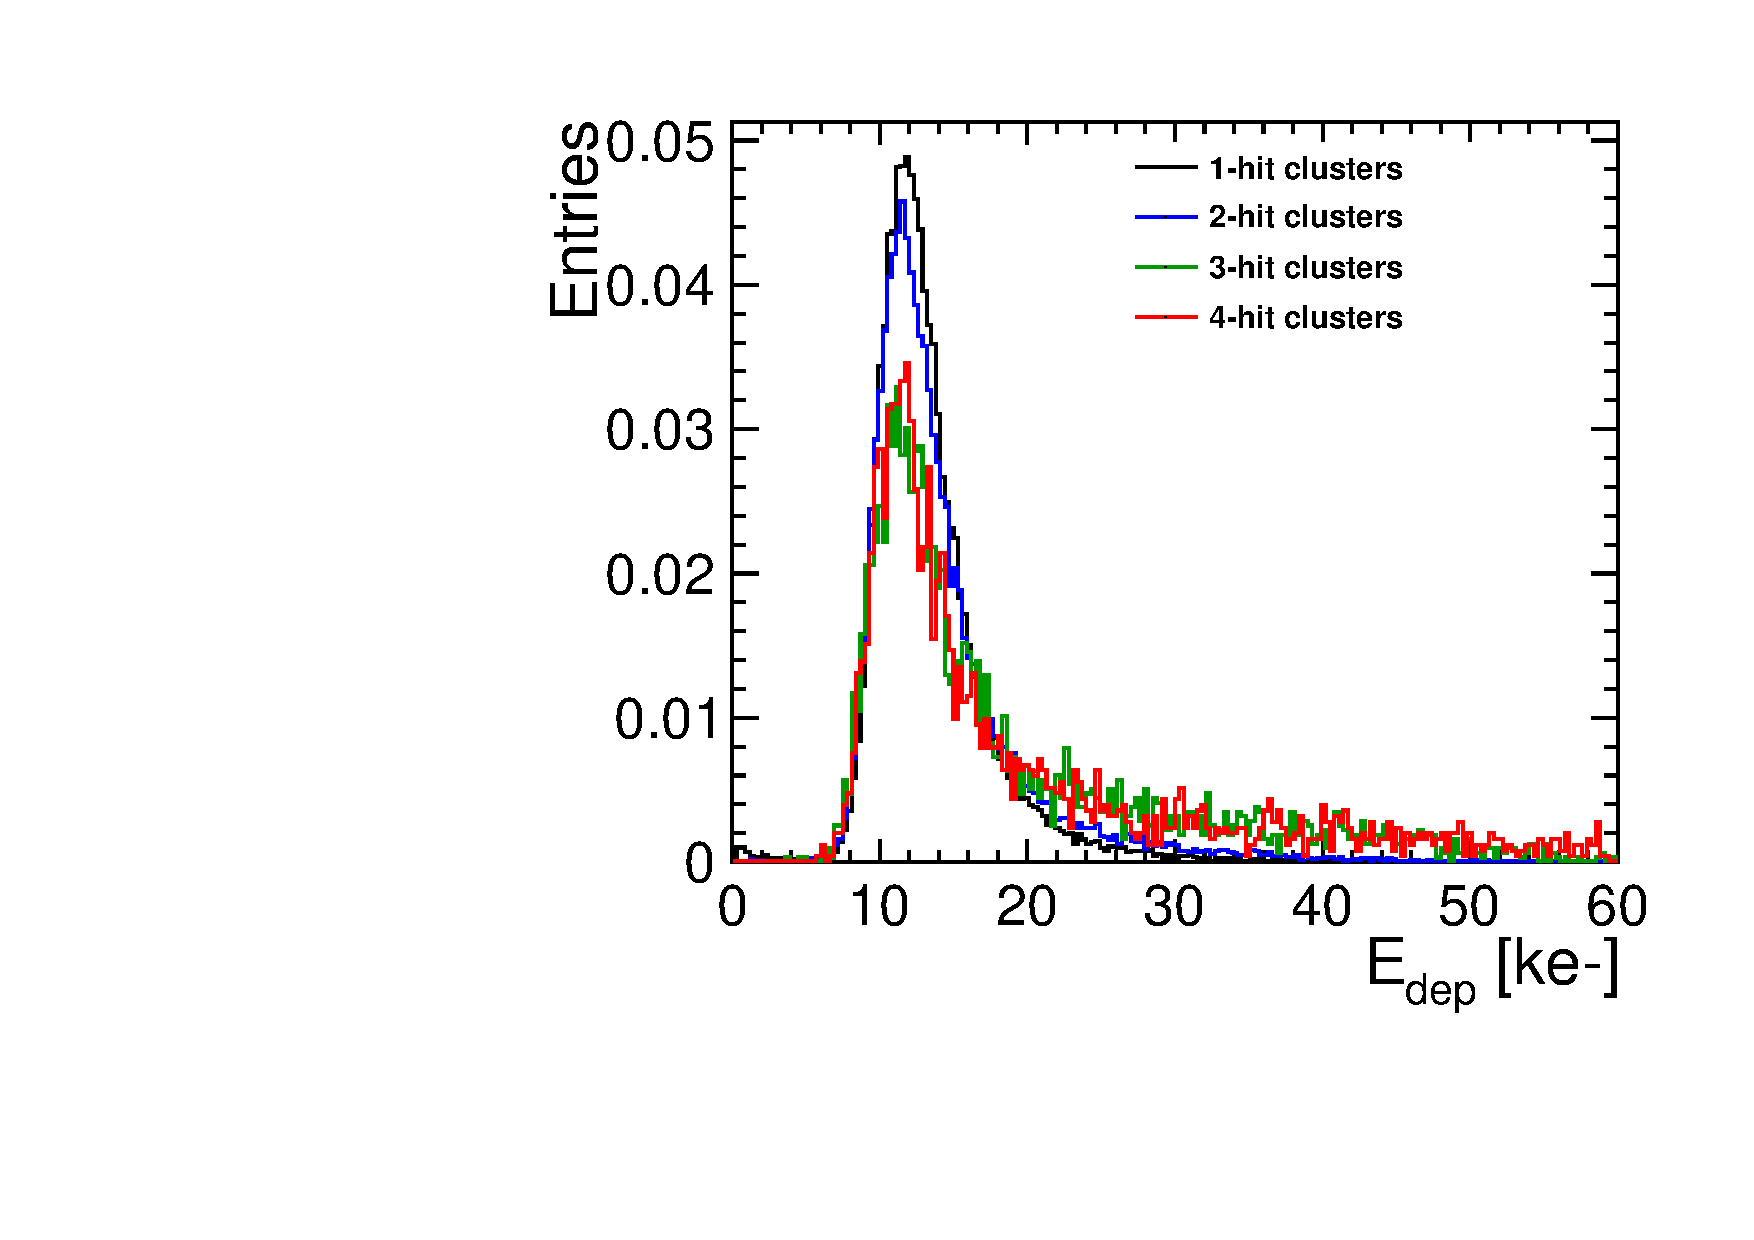
\includegraphics[width=\textwidth]{./figures/Calibration/Edep_Clusters_W0005_F01.pdf}
    \caption{W5\_F1}
  \end{subfigure}
  \caption{Energy deposition distribution for one, two, three and
    four-hit clusters for various assemblies with (a) $50\,\micron$,
    (b) $100\,\micron$ and (c) $150\,\micron$ thick planar sensors.}
  \label{sec:testBeamDataCalibrated_Edep}
\end{figure}

For all the assemblies, the energy deposition in electrons is given in
\cref{sec:appendixCalibDataG4}.


%% --------------------------------------------- %%
\section{Validation of the simulation}
\label{sec:ThinSensorSimuValidation}



The AllPix simulation framework (described in \cref{sec:AllPix}) is
used to simulate the performance of thin sensors and to understand the
charge sharing in such sensors. For the DUT the same digitiser as the
Timepix3 telescope planes is used
(c.f. \cref{sec:allpix_digitisation}). This digitiser takes into
account the semiconductor physics, drift, diffusion charge sharing in
the planar sensors and also noise in the readout ASICs.

The assemblies are simulated at the nominal operating conditions. The
cluster size, the residuals and the energy deposition distributions
are shown in
\cref{fig:G4_simu_data_cluSize,fig:G4_simu_data_Residuals,fig:G4_simu_data_Edep}
comparing data and simulations. The track resolution of
$\sim2\,\micron$ is not unfolded in the residuals distribution. The
simulation is in good agreement with the data and is used to predict
the performance of smaller pixel pitches.

\begin{figure}[htbp] \centering
  \begin{subfigure}[b]{0.23\textwidth}
    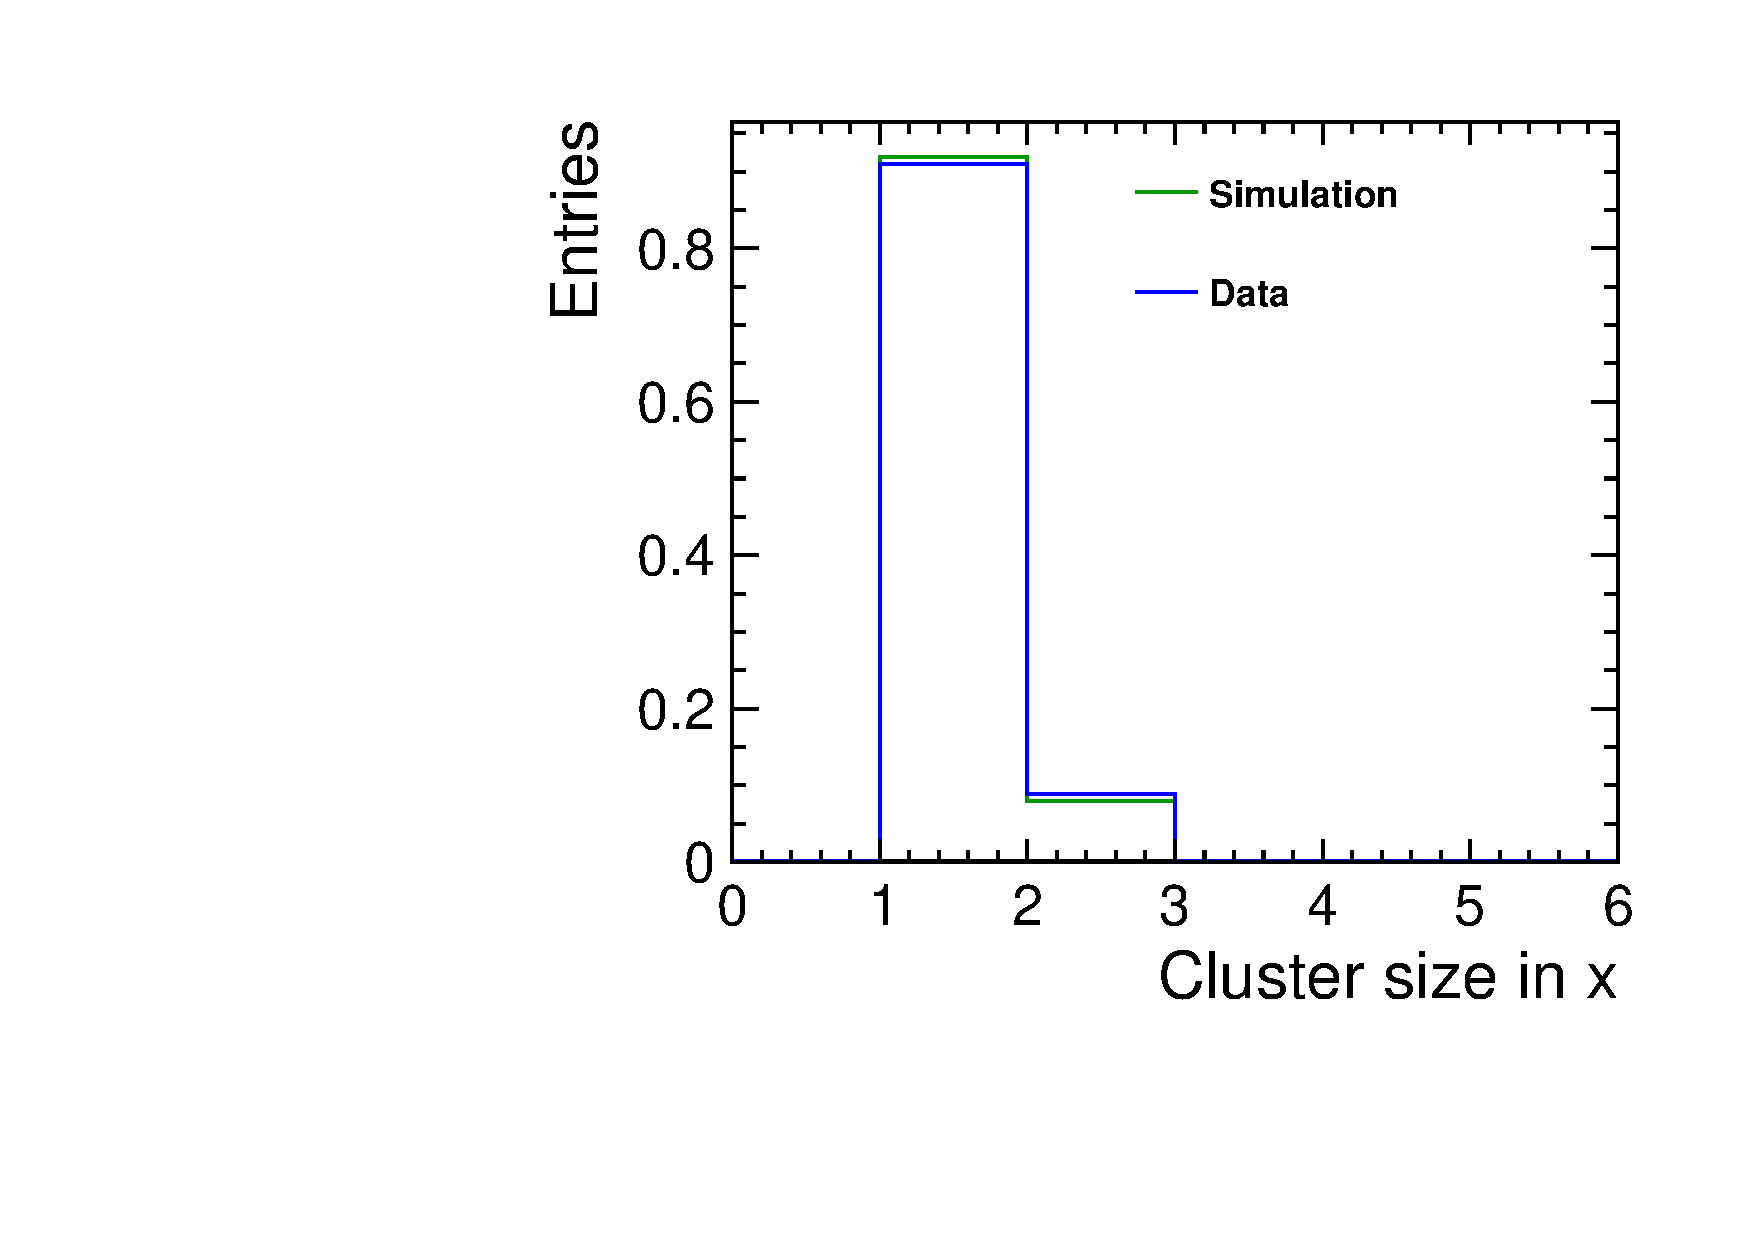
\includegraphics[width=\textwidth]{figures/TestBeam/50micron_sizeX.pdf}
    \caption{$50\,\micron$ n-in-p}
  \end{subfigure} \hfill
  \begin{subfigure}[b]{0.23\textwidth}
    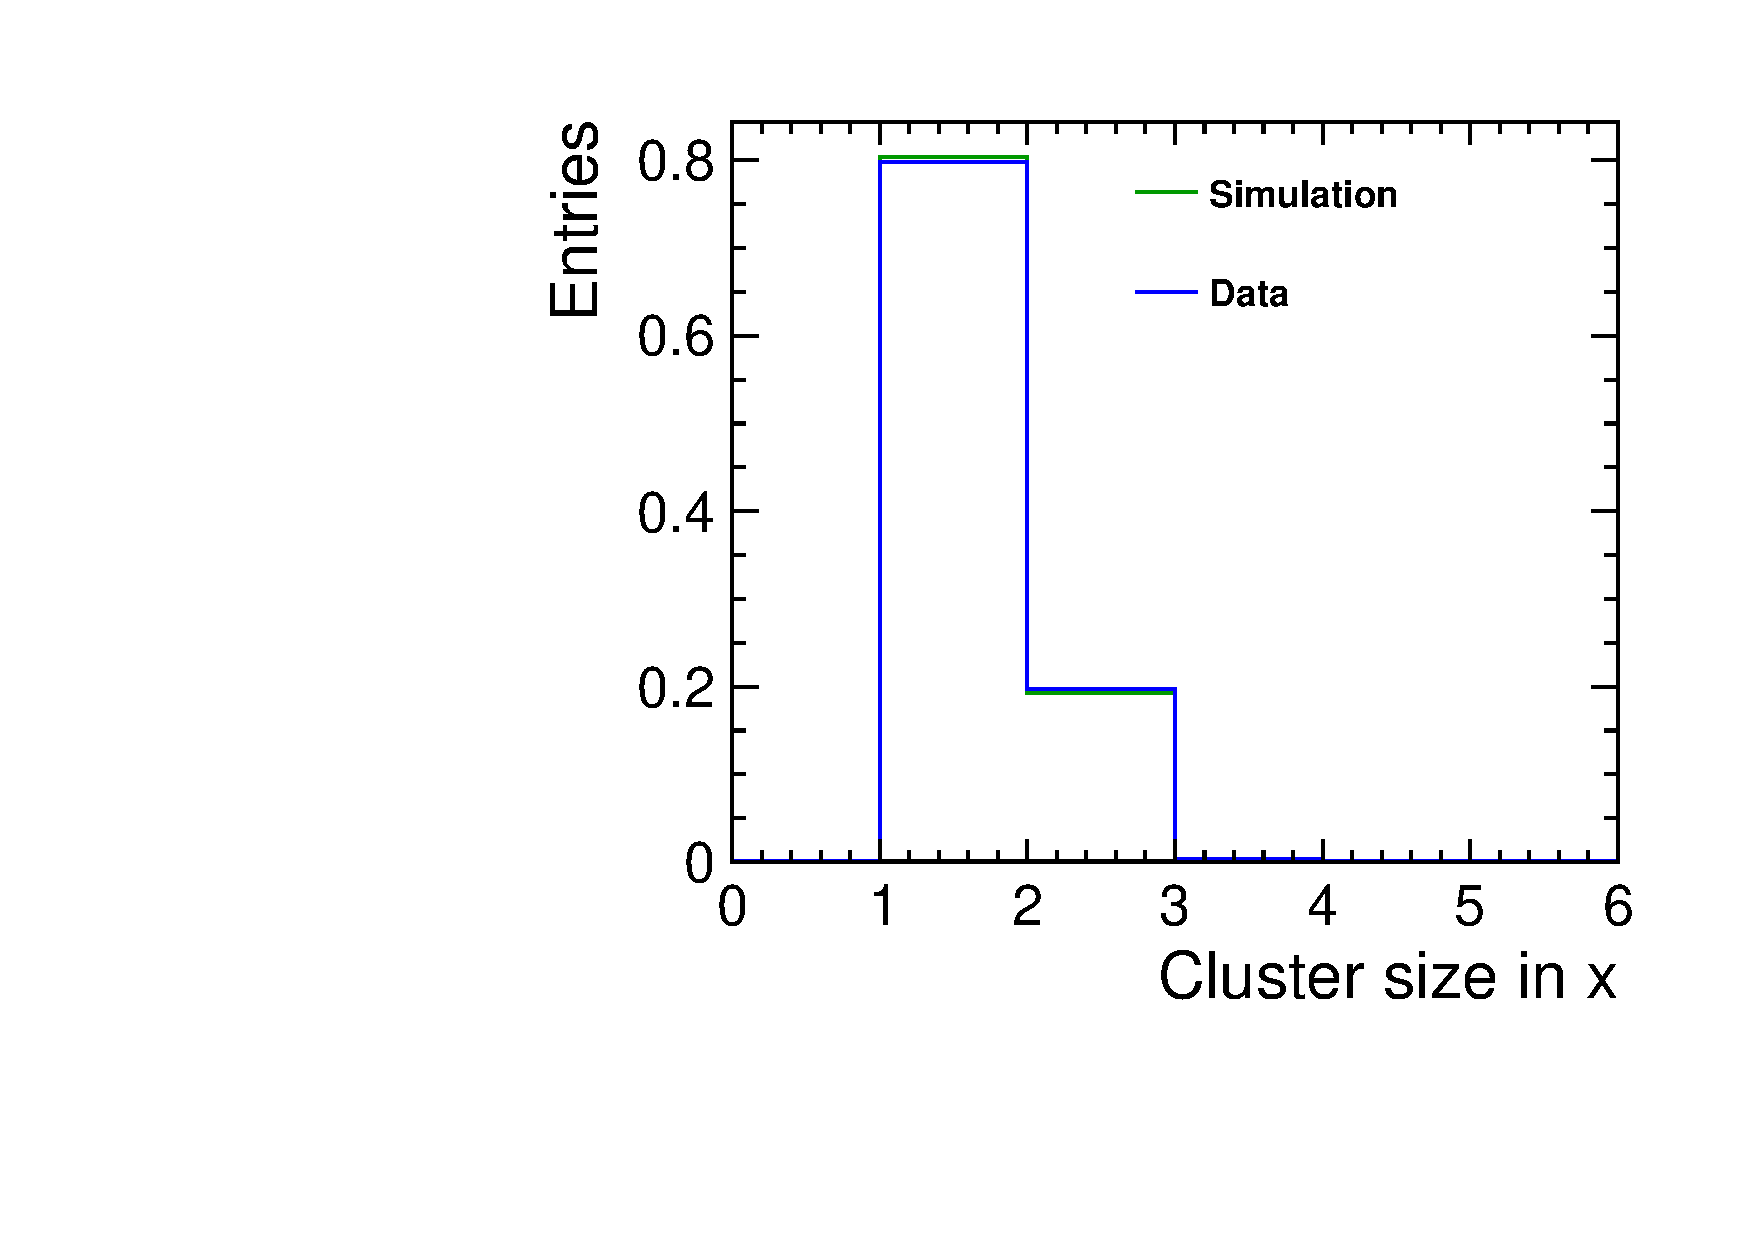
\includegraphics[width=\textwidth]{figures/TestBeam/100micron_sizeX.pdf}
    \caption{$100\,\micron$ n-in-p}
  \end{subfigure} \hfill
  \begin{subfigure}[b]{0.23\textwidth}
    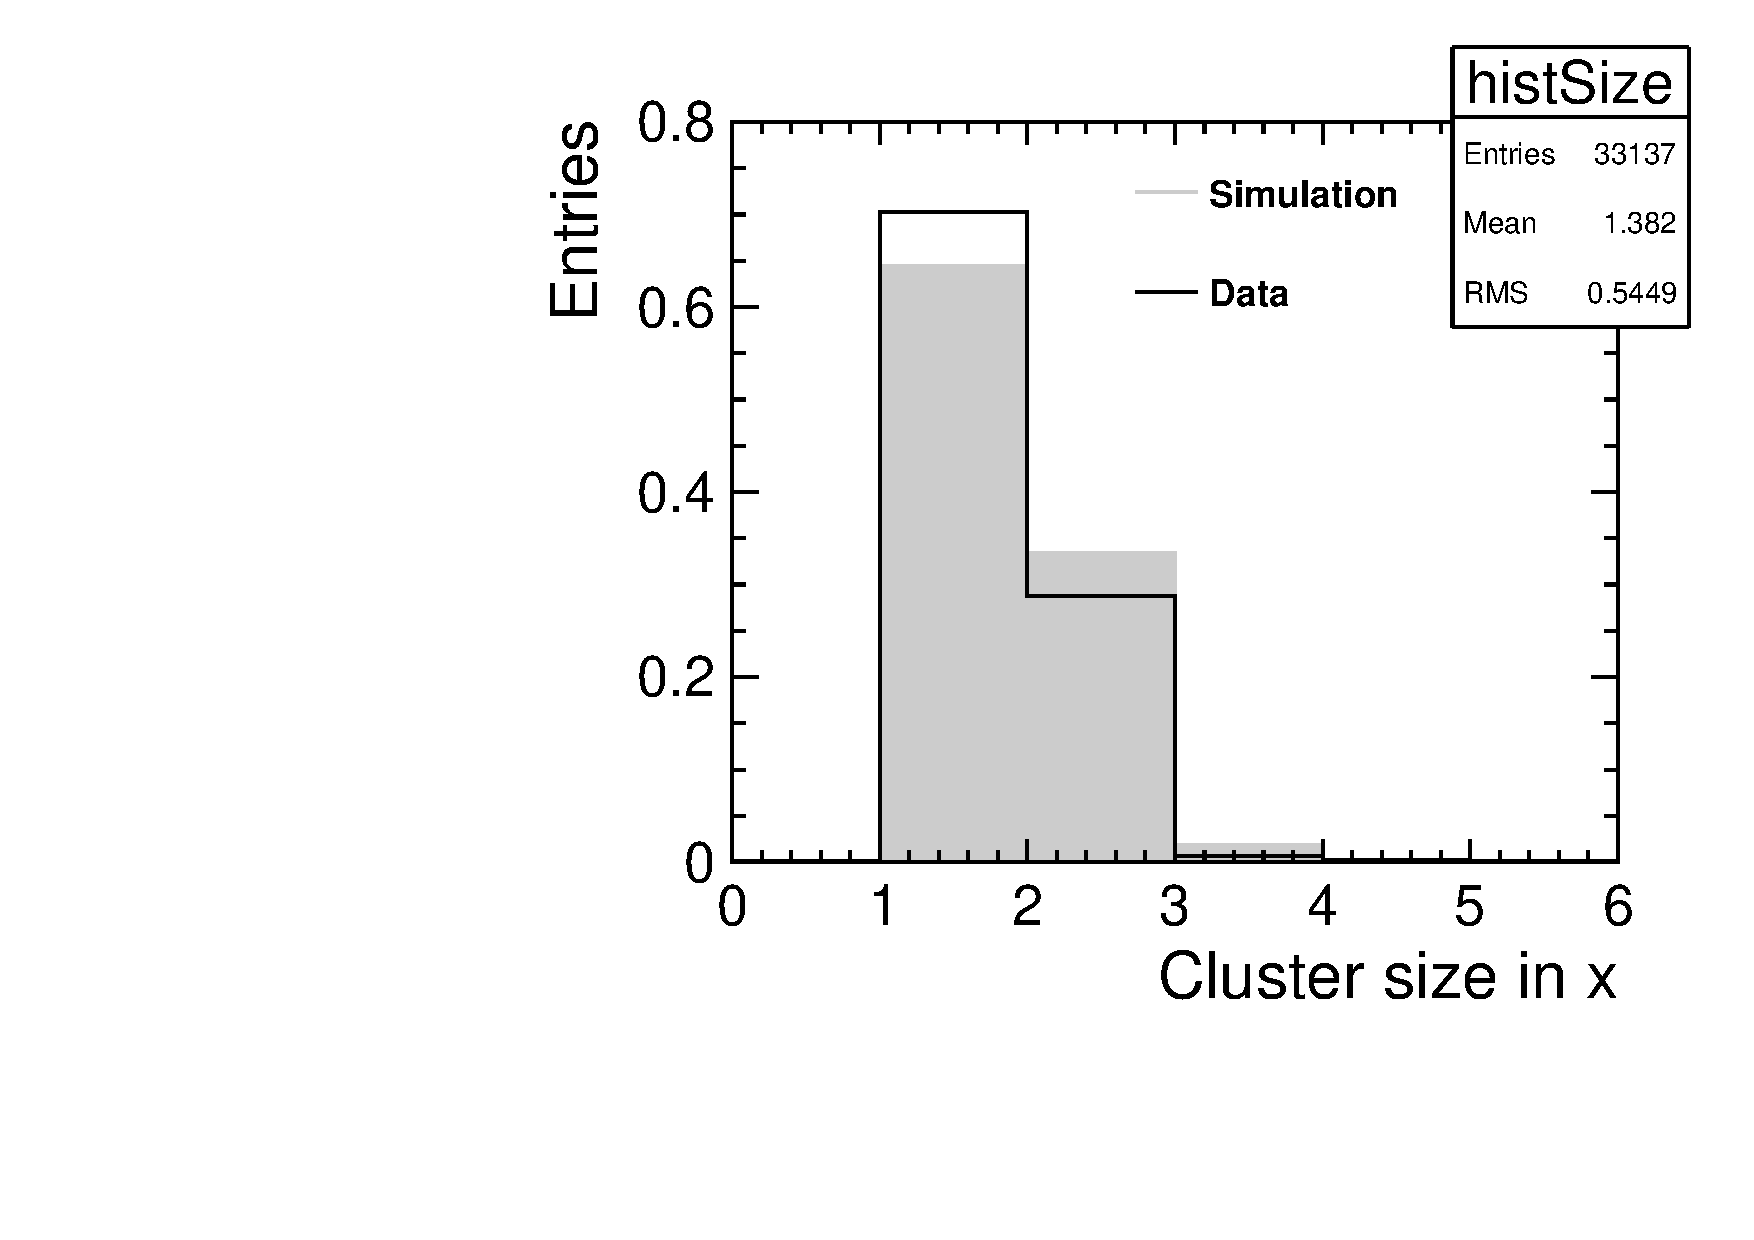
\includegraphics[width=\textwidth]{figures/TestBeam/150micron_sizeX.pdf}
    \caption{$150\,\micron$ n-in-p}
  \end{subfigure} \hfill
  \begin{subfigure}[b]{0.23\textwidth}

    \caption{$300\,\micron$ p-in-n}
  \end{subfigure}
  \caption{The cluster size distribution in simulation and data for
    $50\,\micron$, $100\,\micron$, $150\,\micron$ and $300\,\micron$
    thick sensors. The assemblies are operated at the nominal
    conditions.}
  \label{fig:G4_simu_data_cluSize}
\end{figure}

\begin{figure}[htbp] \centering
  \begin{subfigure}[b]{0.23\textwidth}
    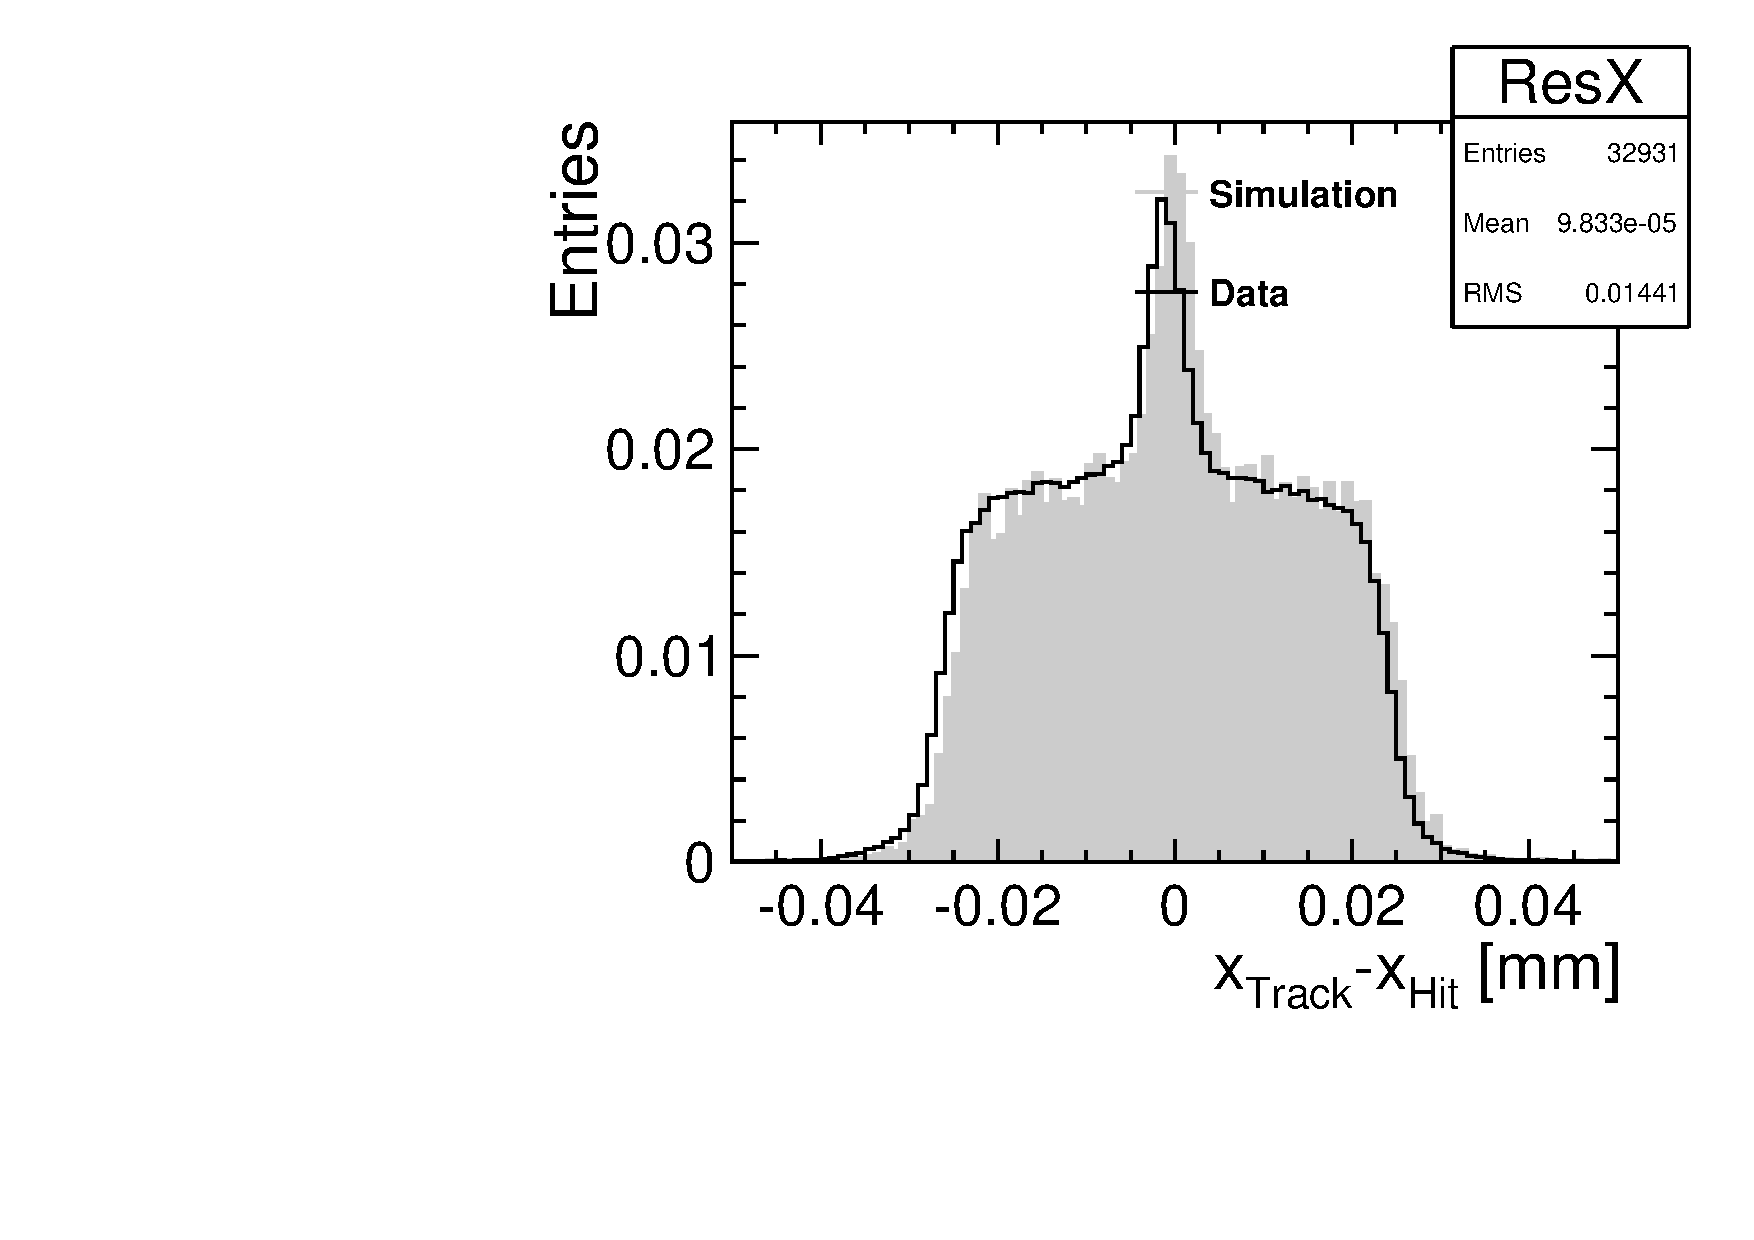
\includegraphics[width=\textwidth]{figures/TestBeam/50micron_resX.pdf}
    \caption{$50\,\micron$ n-in-p}
  \end{subfigure} \hfill
  \begin{subfigure}[b]{0.23\textwidth}
    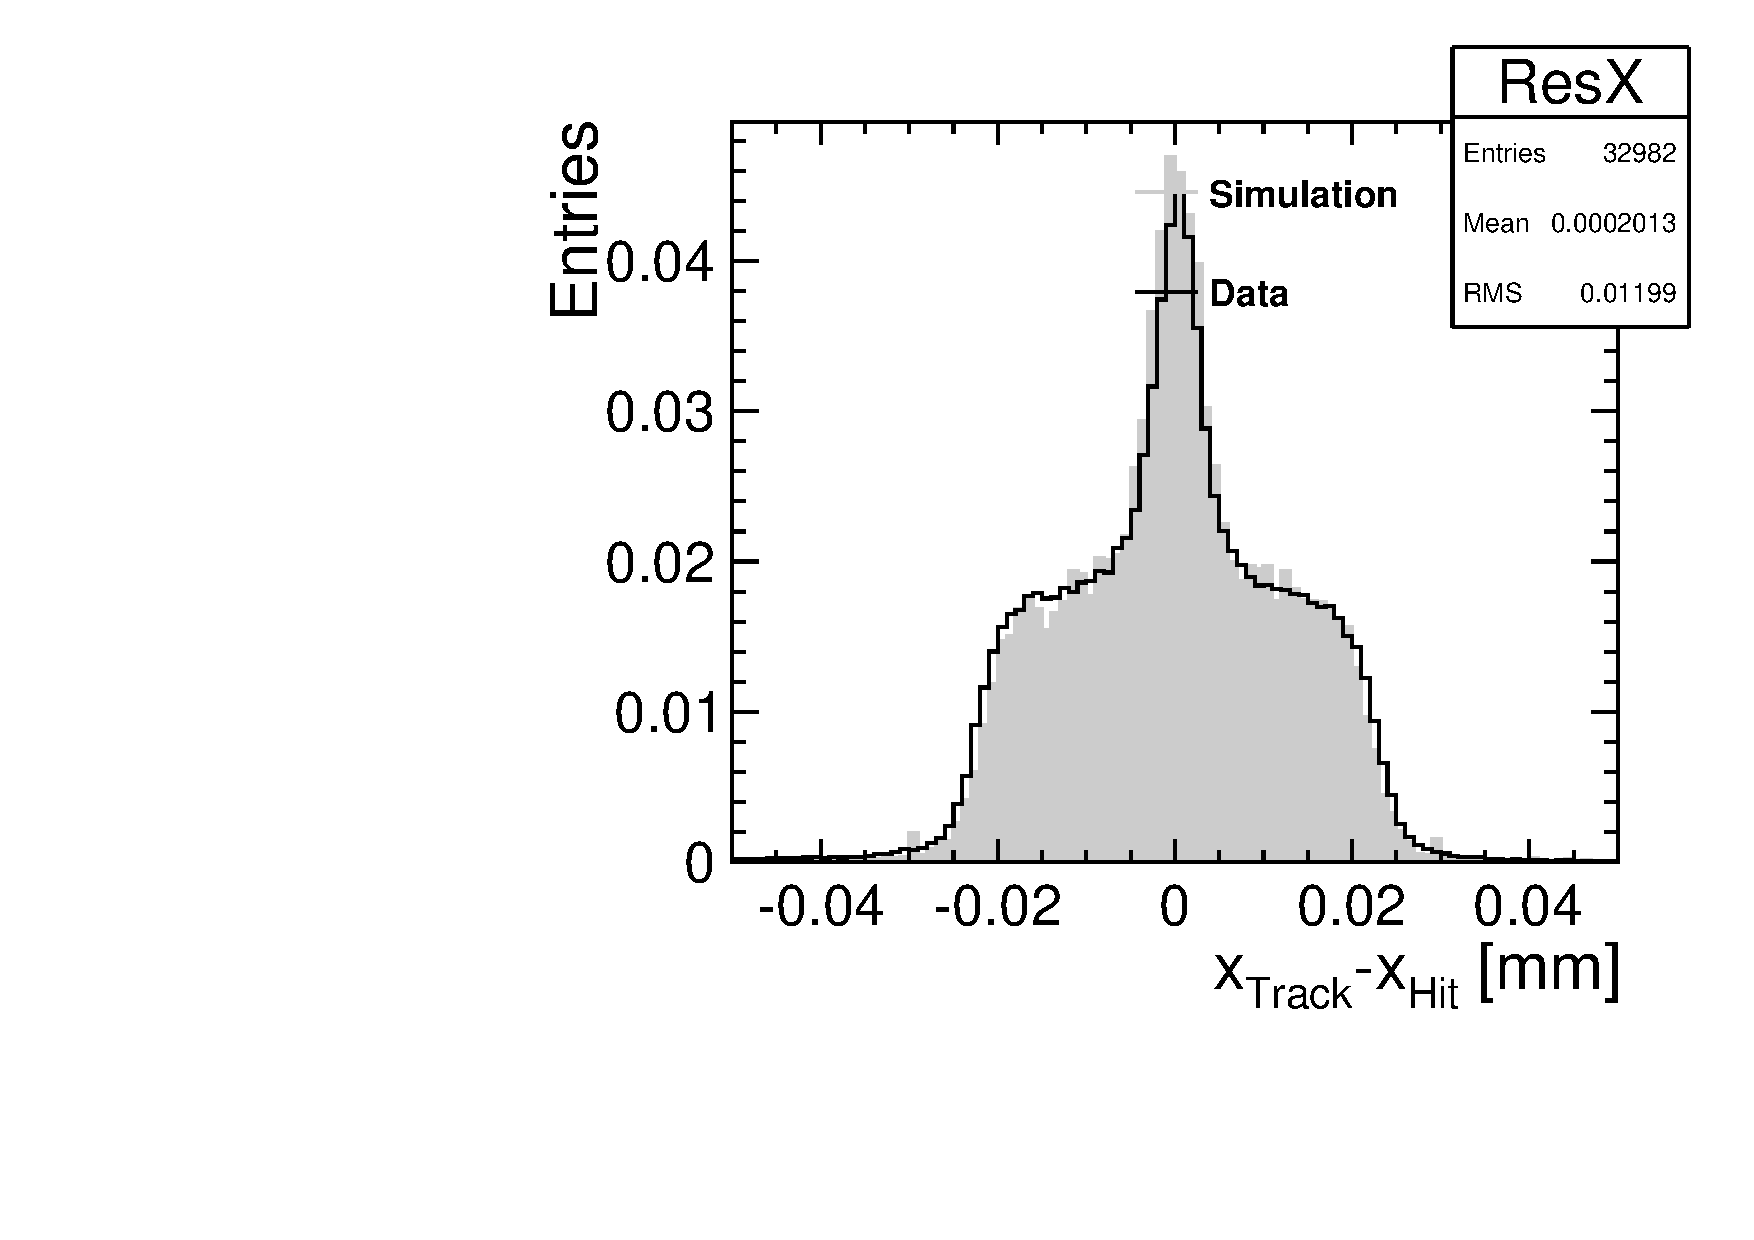
\includegraphics[width=\textwidth]{figures/TestBeam/100micron_resX.pdf}
    \caption{$100\,\micron$ n-in-p}
  \end{subfigure} \hfill
  \begin{subfigure}[b]{0.23\textwidth}
    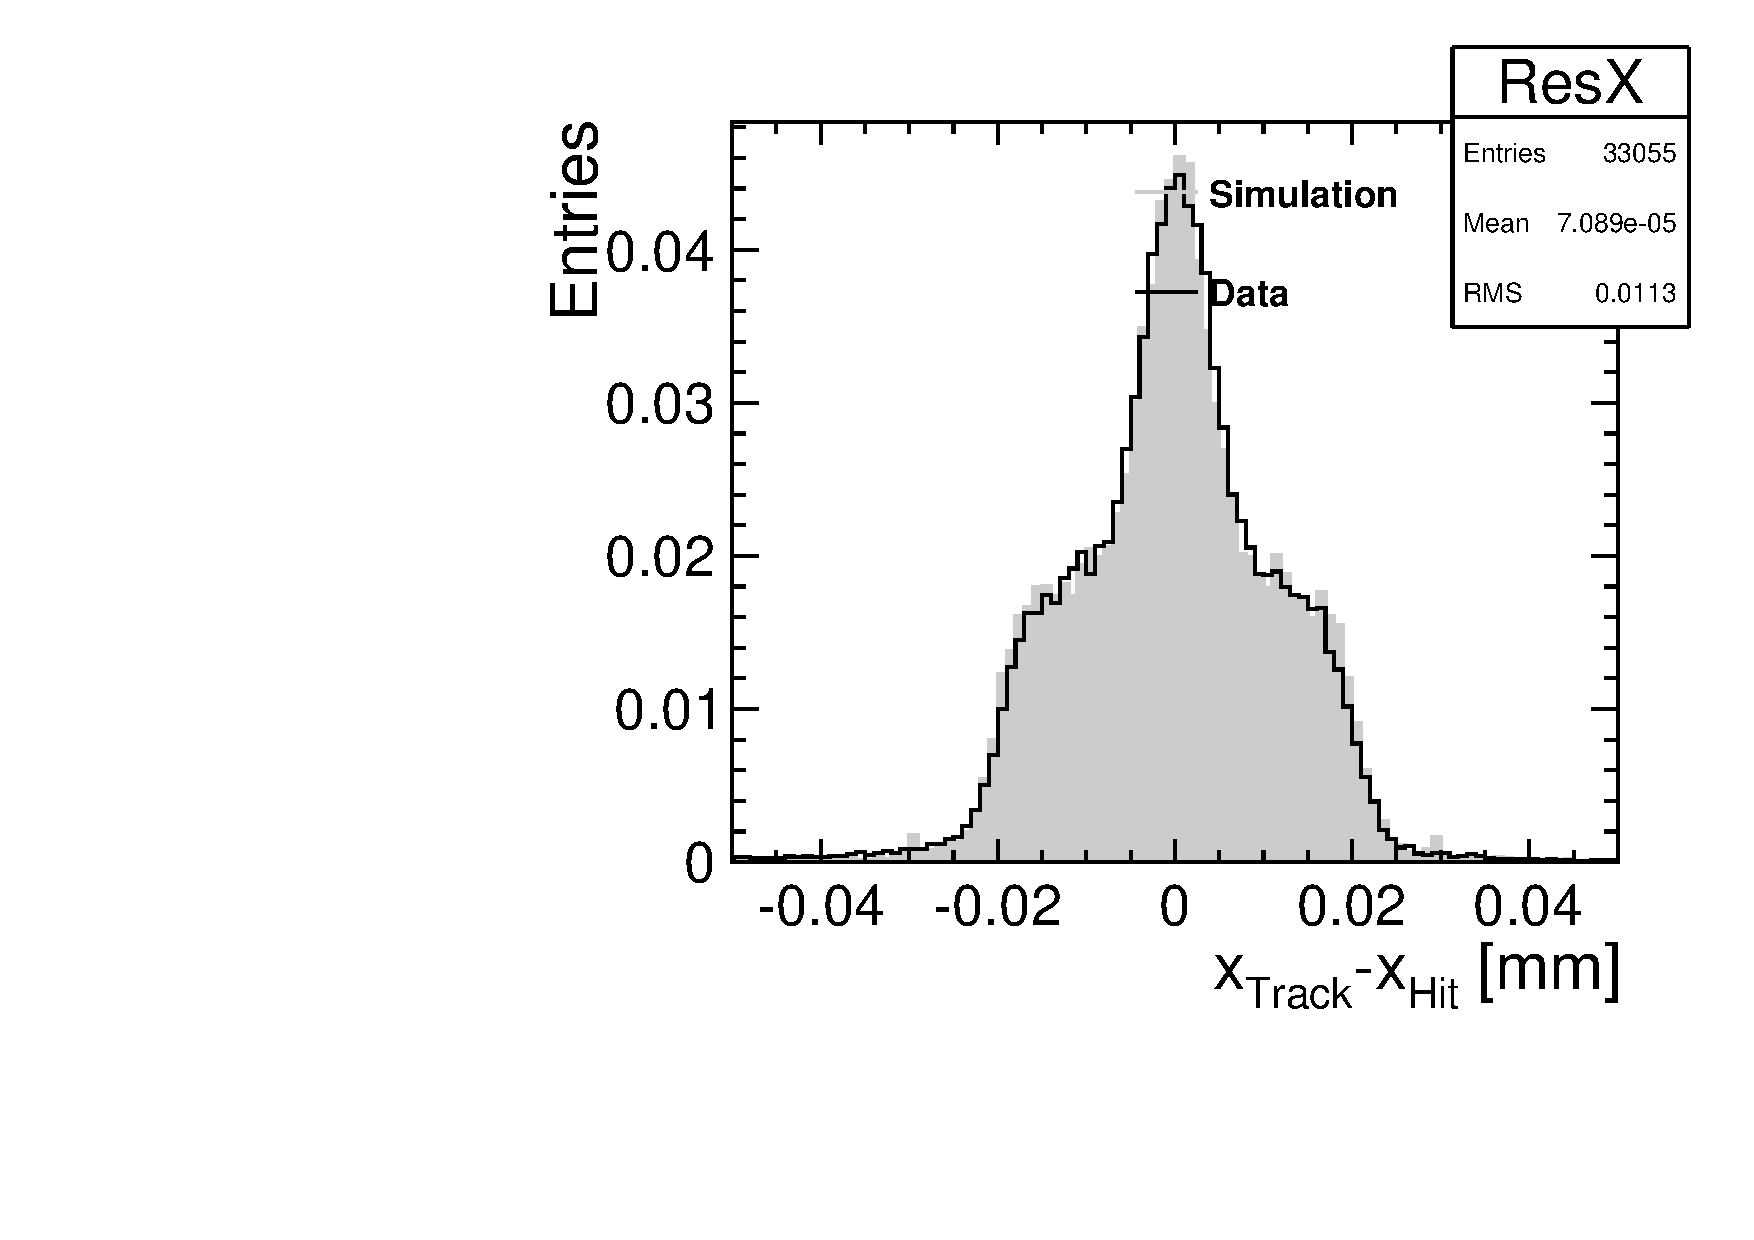
\includegraphics[width=\textwidth]{figures/TestBeam/150micron_resX.pdf}
    \caption{$150\,\micron$ n-in-p}
  \end{subfigure} \hfill
  \begin{subfigure}[b]{0.23\textwidth}

    \caption{$300\,\micron$ p-in-n}
  \end{subfigure}
  \caption{The residuals distribution in simulation and data for
    $50\,\micron$, $100\,\micron$, $150\,\micron$ and $300\,\micron$
    thick sensors. The assemblies are operated at the nominal
    conditions. The tracking resolution is not unfolded.}
  \label{fig:G4_simu_data_Residuals}
\end{figure}

\begin{figure}[htbp] \centering
  \begin{subfigure}[b]{0.23\textwidth}
    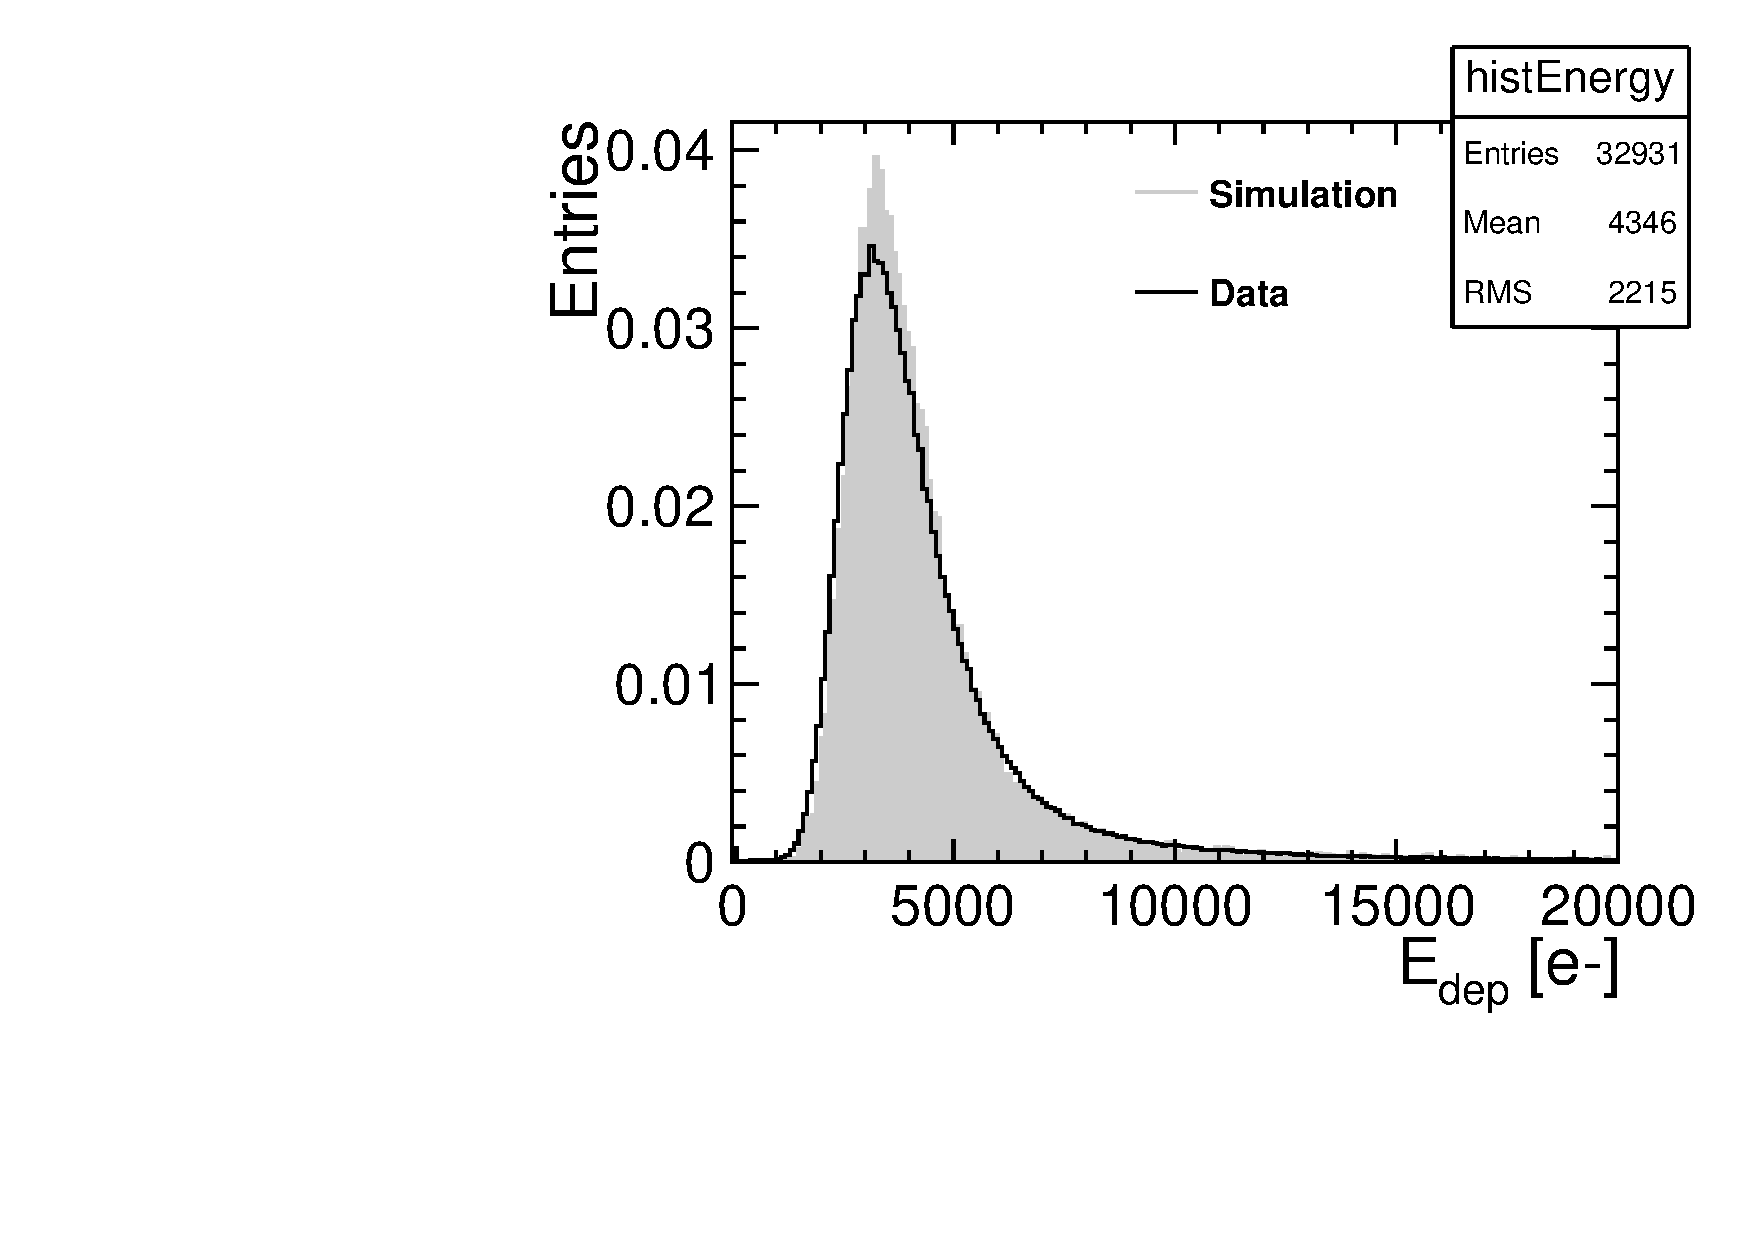
\includegraphics[width=\textwidth]{figures/TestBeam/50micron_Edep.pdf}
    \caption{$50\,\micron$ n-in-p}
  \end{subfigure} \hfill
  \begin{subfigure}[b]{0.23\textwidth}
    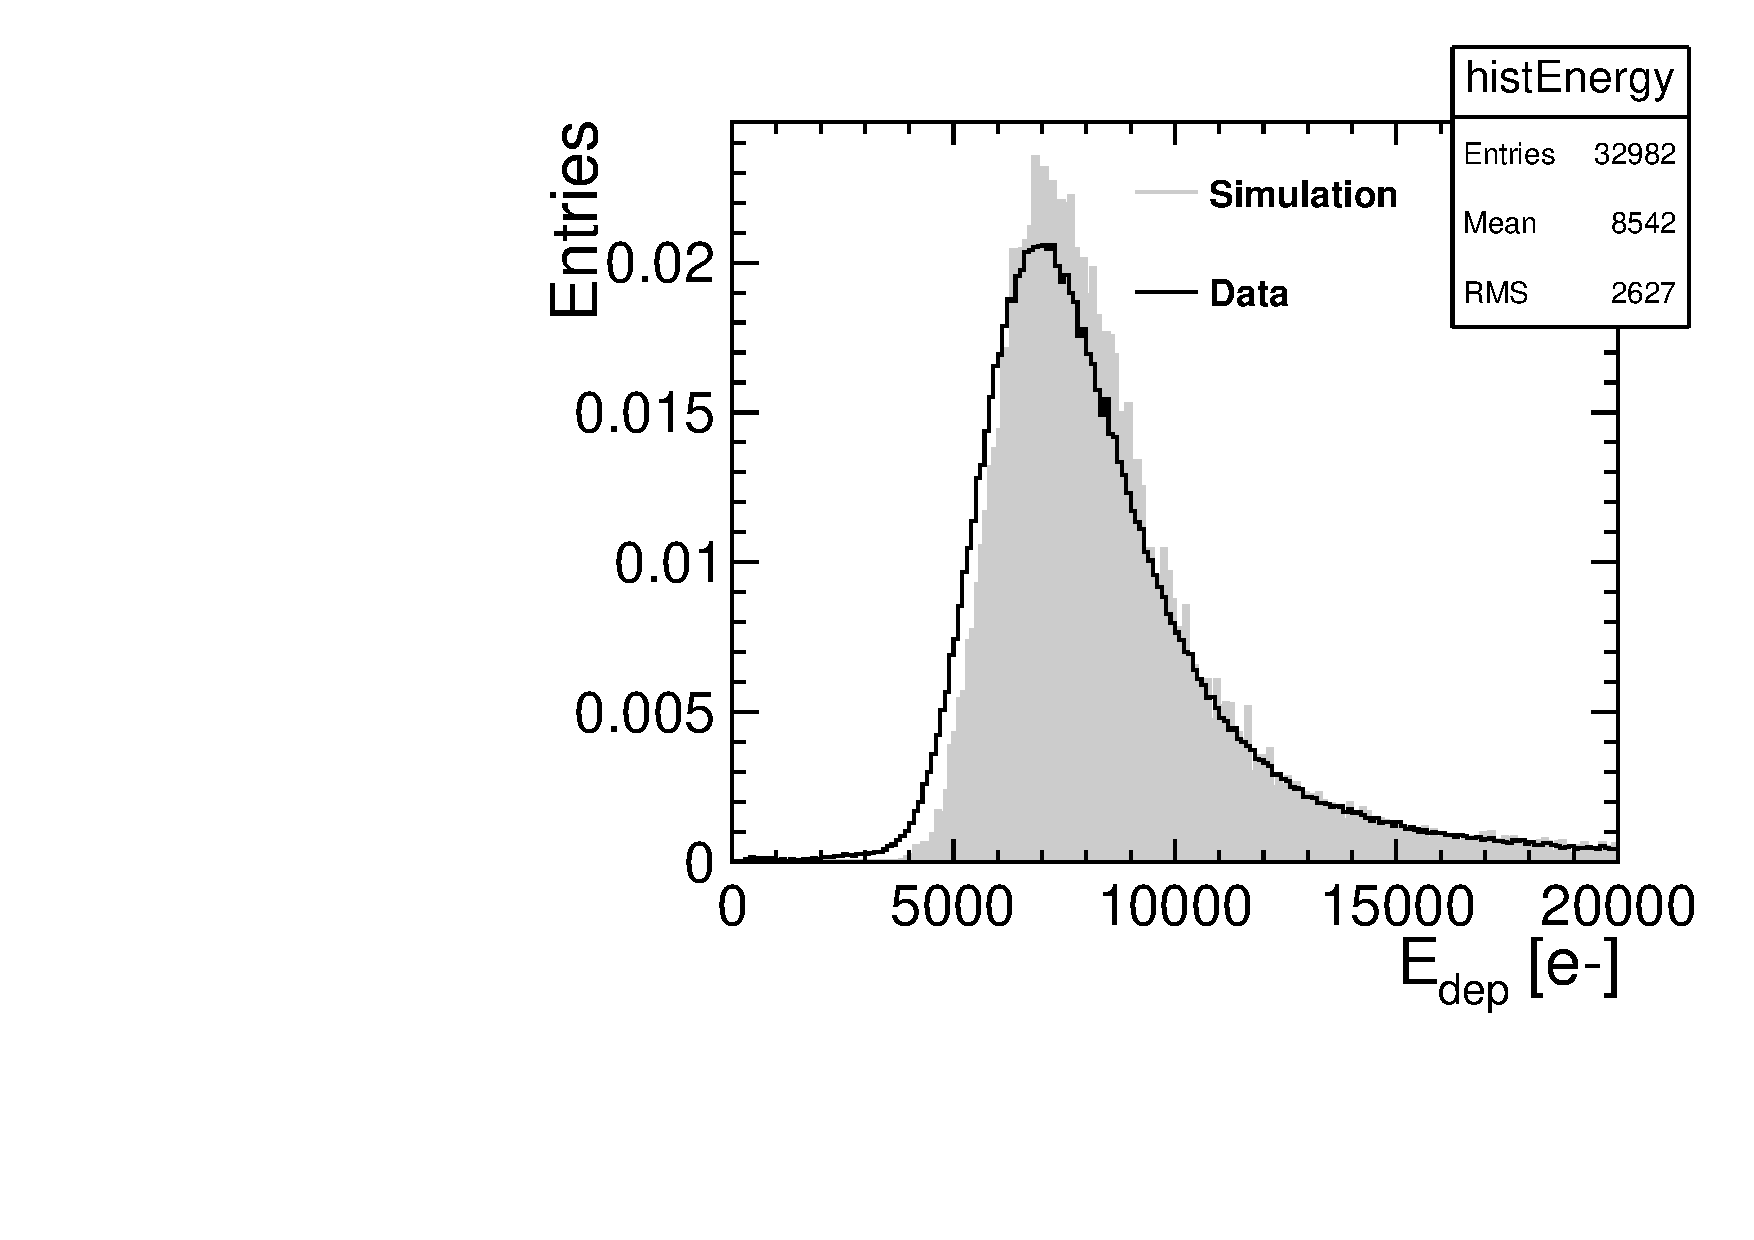
\includegraphics[width=\textwidth]{figures/TestBeam/100micron_Edep.pdf}
    \caption{$100\,\micron$ n-in-p}
  \end{subfigure} \hfill
  \begin{subfigure}[b]{0.23\textwidth}
    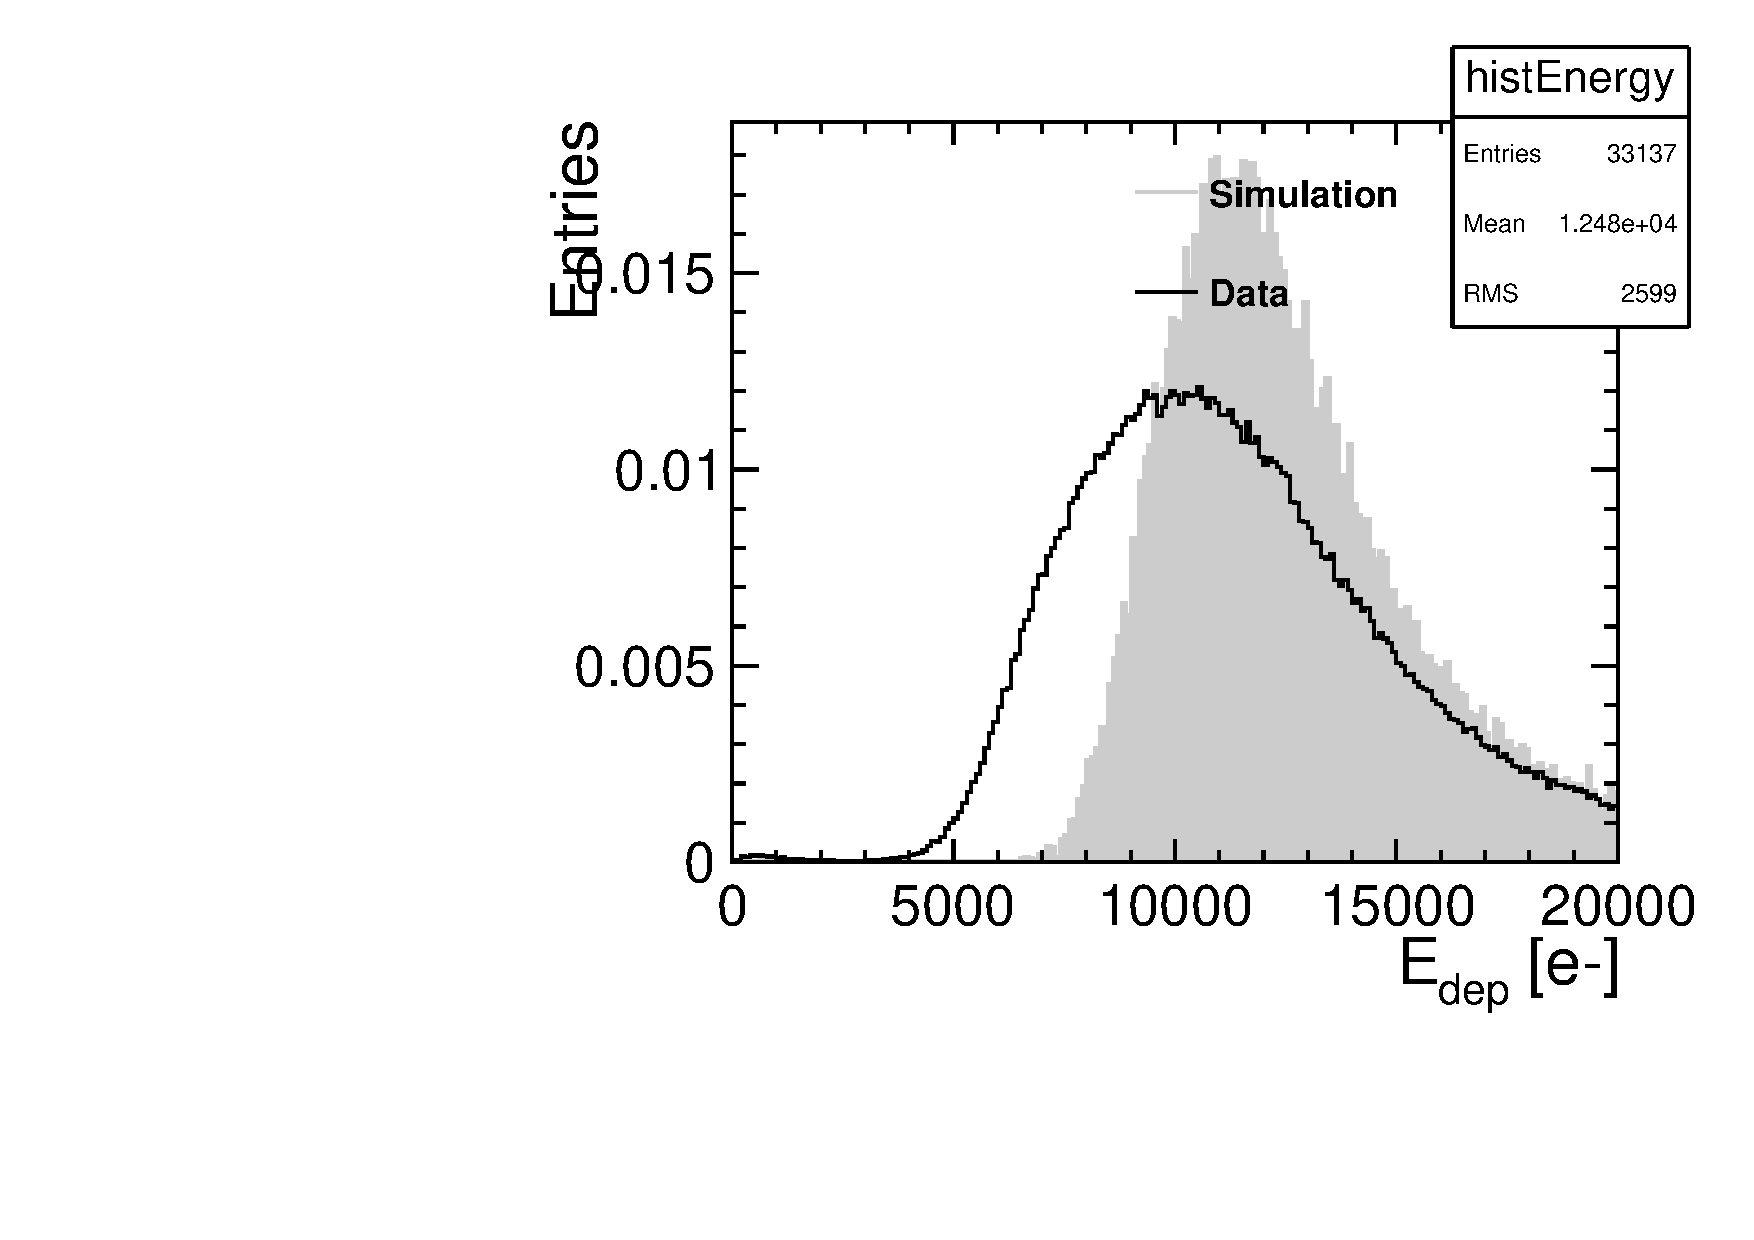
\includegraphics[width=\textwidth]{figures/TestBeam/150micron_Edep.pdf}
    \caption{$150\,\micron$ n-in-p}
  \end{subfigure} \hfill
  \begin{subfigure}[b]{0.23\textwidth}

    \caption{$300\,\micron$ p-in-n}
  \end{subfigure}
  \caption{The energy deposition for all cluster sizes in simulation
    and data for $50\,\micron$, $100\,\micron$, $150\,\micron$ and
    $300\,\micron$ thick sensors. The assemblies are operated at the
    nominal conditions.}
  \label{fig:G4_simu_data_Edep}
\end{figure}

%% --------------------------------------------- %%
\section{Extrapolation to smaller pixels (CLICpix)}

Figure~\ref{fig:cluSize25Pitch} shows the cluster-size distribution
and the hit residuals for an extrapolation of the simulation to
$25\,\micron$ pitch pixels with $50\,\micron$ thick sensors with a
Timepix3-type readout chip operated at 500 electrons threshold with
10-bit TOT measurement and an electronic noise of $\sim$90
electrons. The same digitiser as the one used to validate the
simulation in \cref{sec:ThinSensorSimuValidation} is used for the
extrapolation. Even with a small pitch, in such thin sensors, only
$\sim$16\% of clusters originating from minimum ionising particles
contain more than one pixel. The residual distribution is therefore
dominated by the broad peak from single-pixel clusters and the
resulting resolution of $\sim6\,\micron$ (with the unfolded tracking
resolution) is still significantly worse than the required
$3\,\micron$. It can be concluded that the required resolution can be
either obtained with smaller pixels using planar sensors or new
solution of charge sharing are needed in order to reduce even more the
number of single-hit clusters. By tilting the detectors, the charge
sharing could be as well optimised.

\begin{figure}[htbp]\centering
  \begin{subfigure}[b]{0.45\textwidth}
    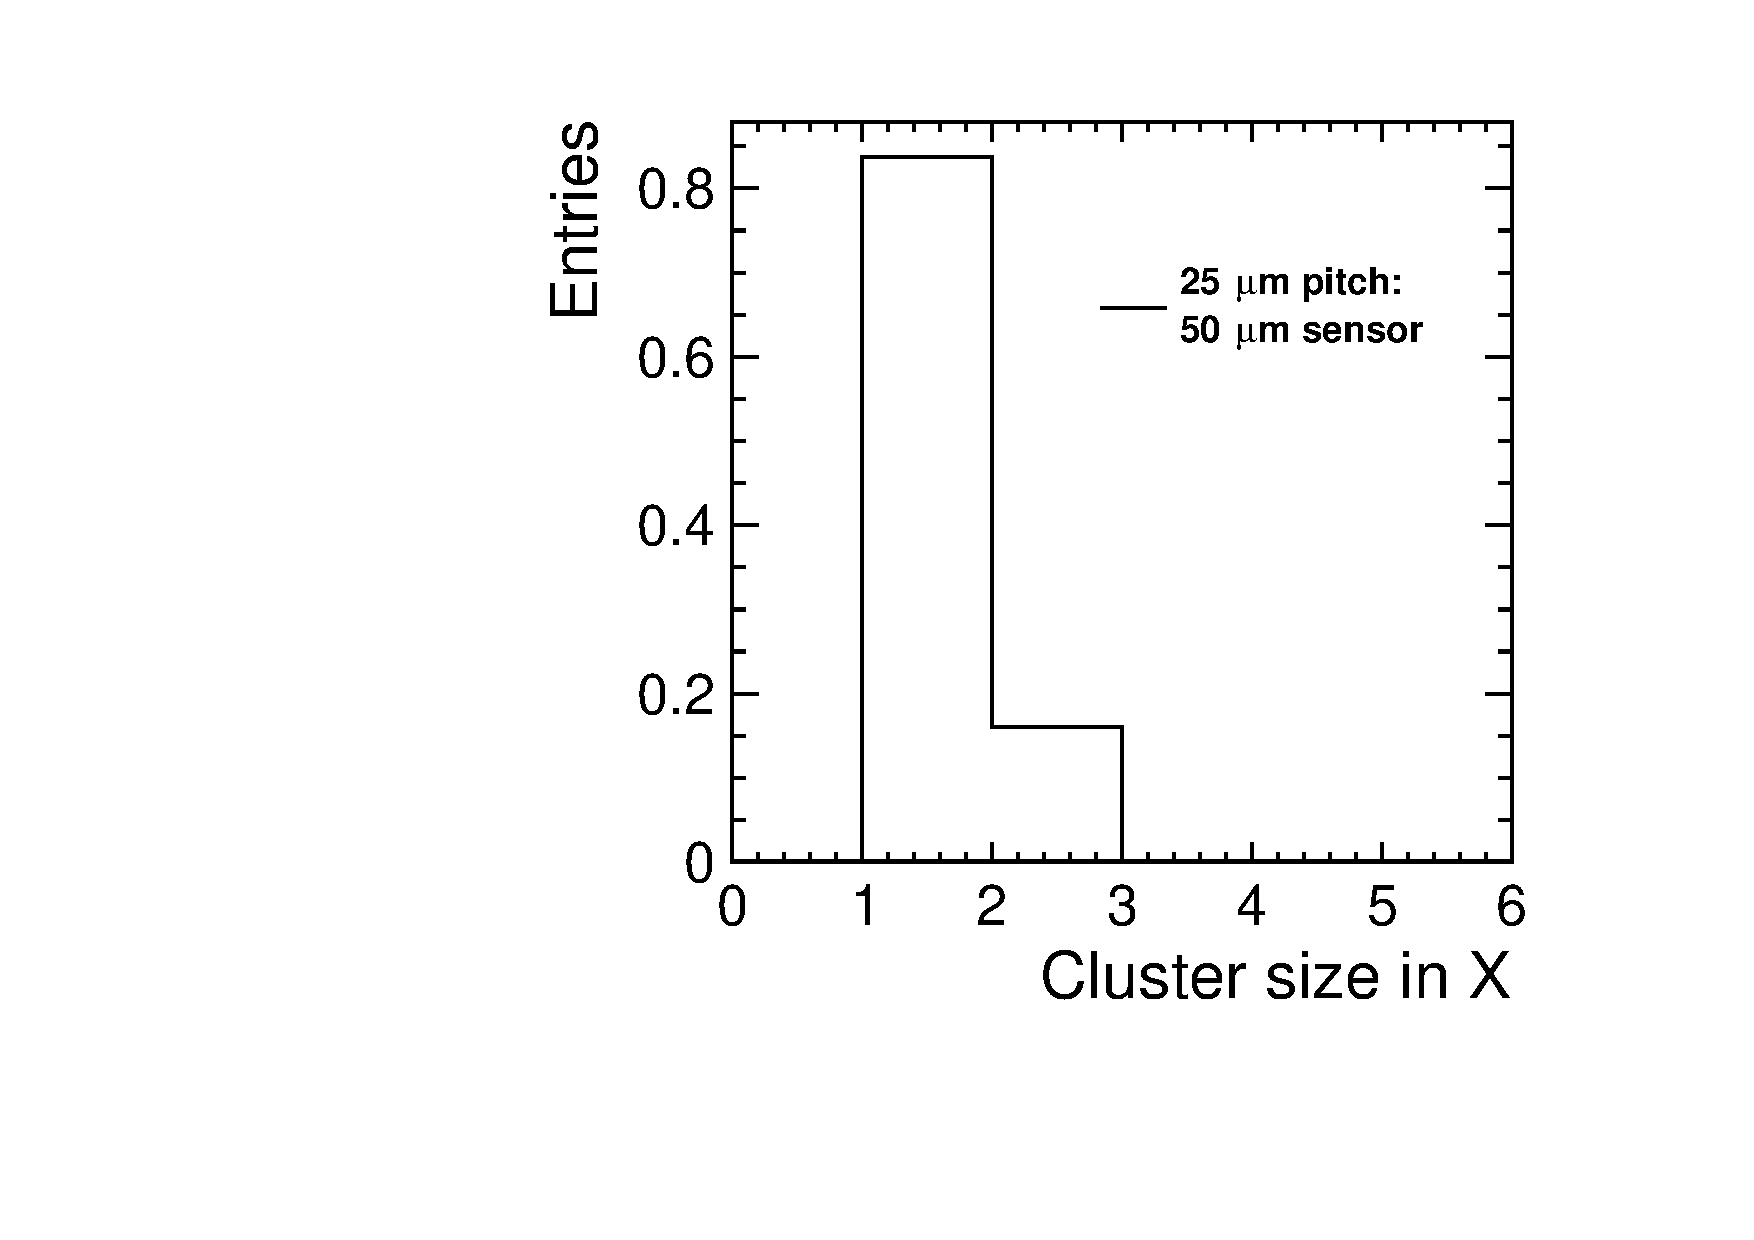
\includegraphics[width=\textwidth]{figures/TestBeam/ClusterSize_TPX3_CLICpix.pdf}
    \caption{}
  \end{subfigure}\hfill
  \begin{subfigure}[b]{0.45\textwidth}
    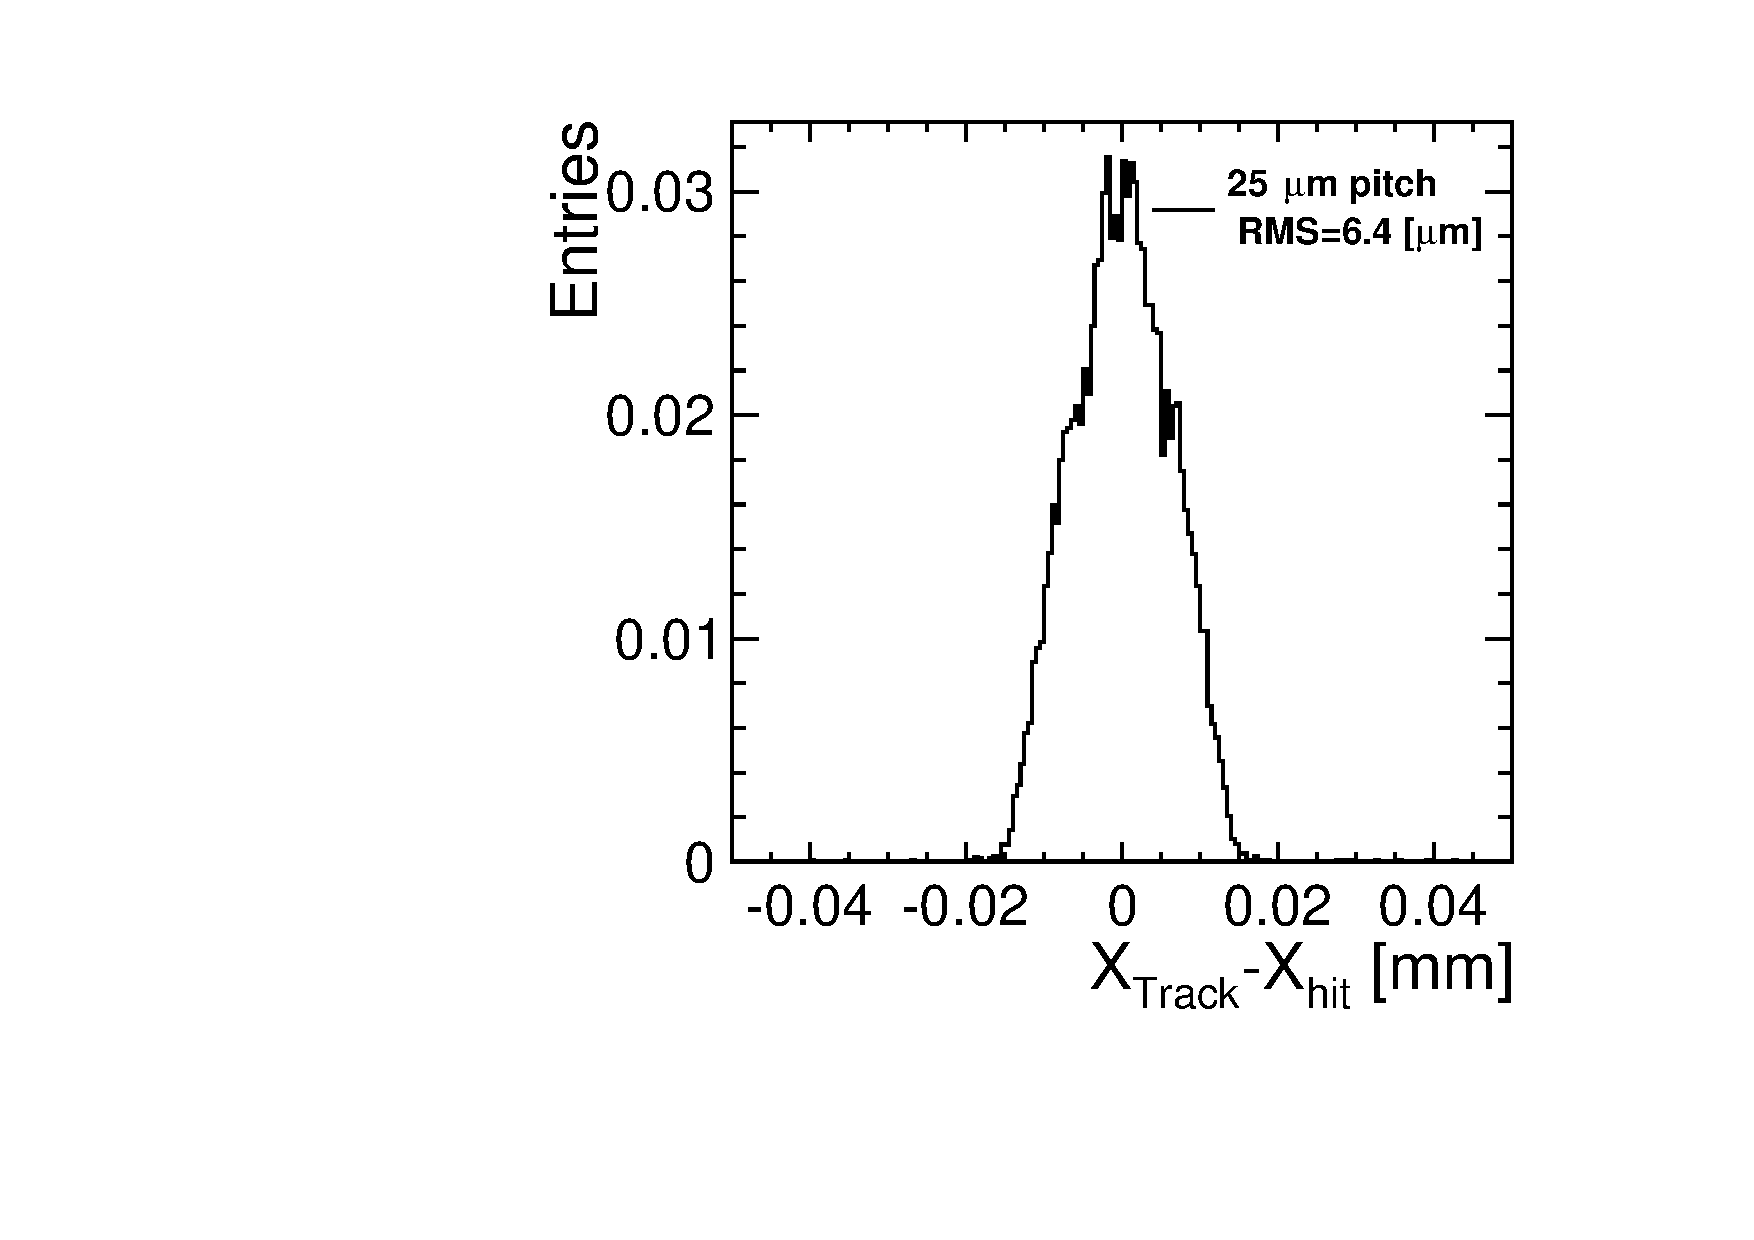
\includegraphics[width=\textwidth]{figures/TestBeam/ResolutionX_TPX3_CLICpix.pdf}
    \caption{}
  \end{subfigure}
  \caption{(a) Cluster-size distribution and (b) hit residuals in
    x-direction for the extrapolation of the simulation to
    $25\,\micron$ pixel pitch with a $50\,\micron$ thick sensor and a
    threshold of $\sim$500 electrons.}
  \label{fig:cluSize25Pitch}
\end{figure}


%% \begin{figure}[htbp] 
%%   \centering
%%   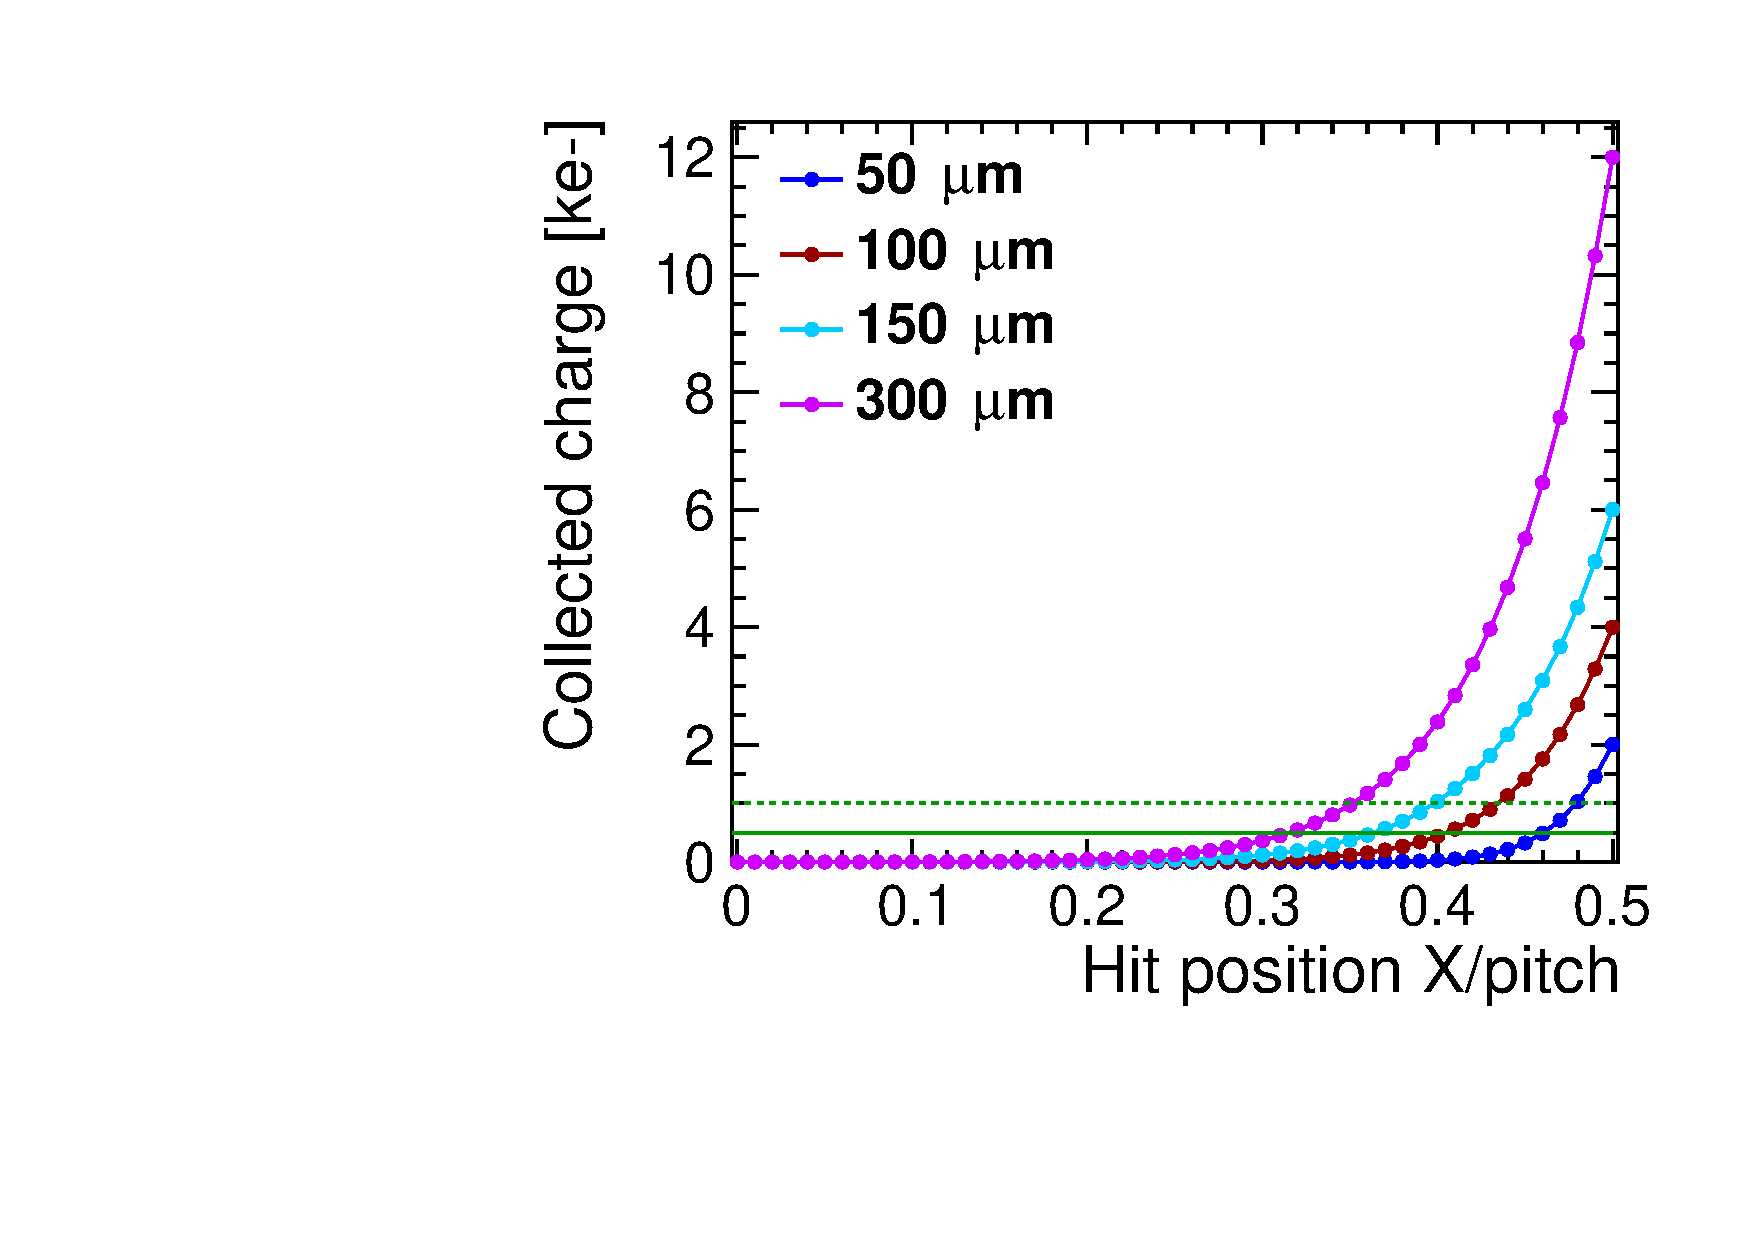
\includegraphics[width=0.5\textwidth]{./figures/TestBeam/chargeSharing_theory.pdf}
%%   \caption{Thresholds at 500 at 1000 electrons are shown in green lines.}
%%   \label{fig:chargeSharing_theory}
%% \end{figure}

%% %% --------------------------------------------- %%
%% \begin{figure}[htbp] \centering
%%   \begin{subfigure}[b]{0.45\textwidth}
%%     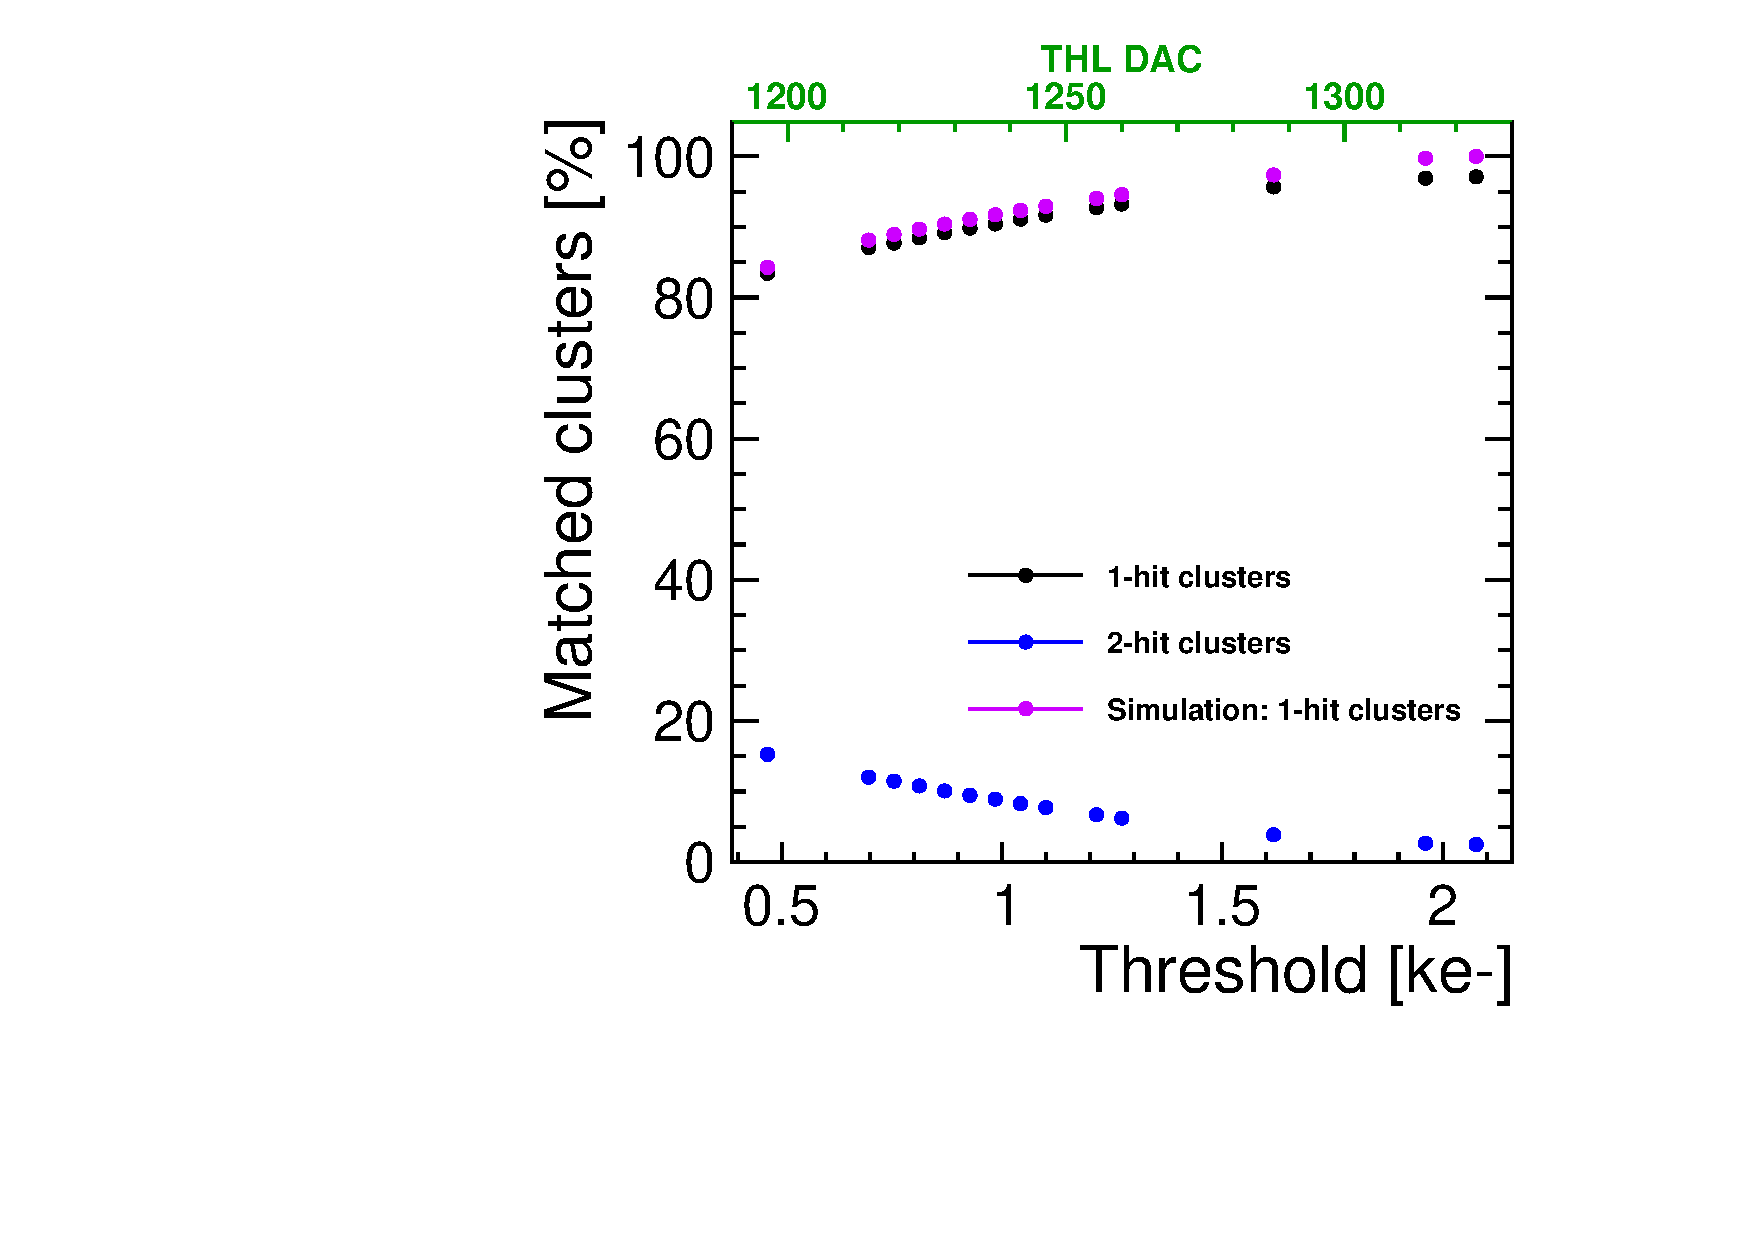
\includegraphics[width=\textwidth]{./figures/TestBeam/ThresholdScan_W0019_G07.pdf}
%%     \caption{}
%%   \end{subfigure} \hfill
%%   \begin{subfigure}[b]{0.45\textwidth}
%%     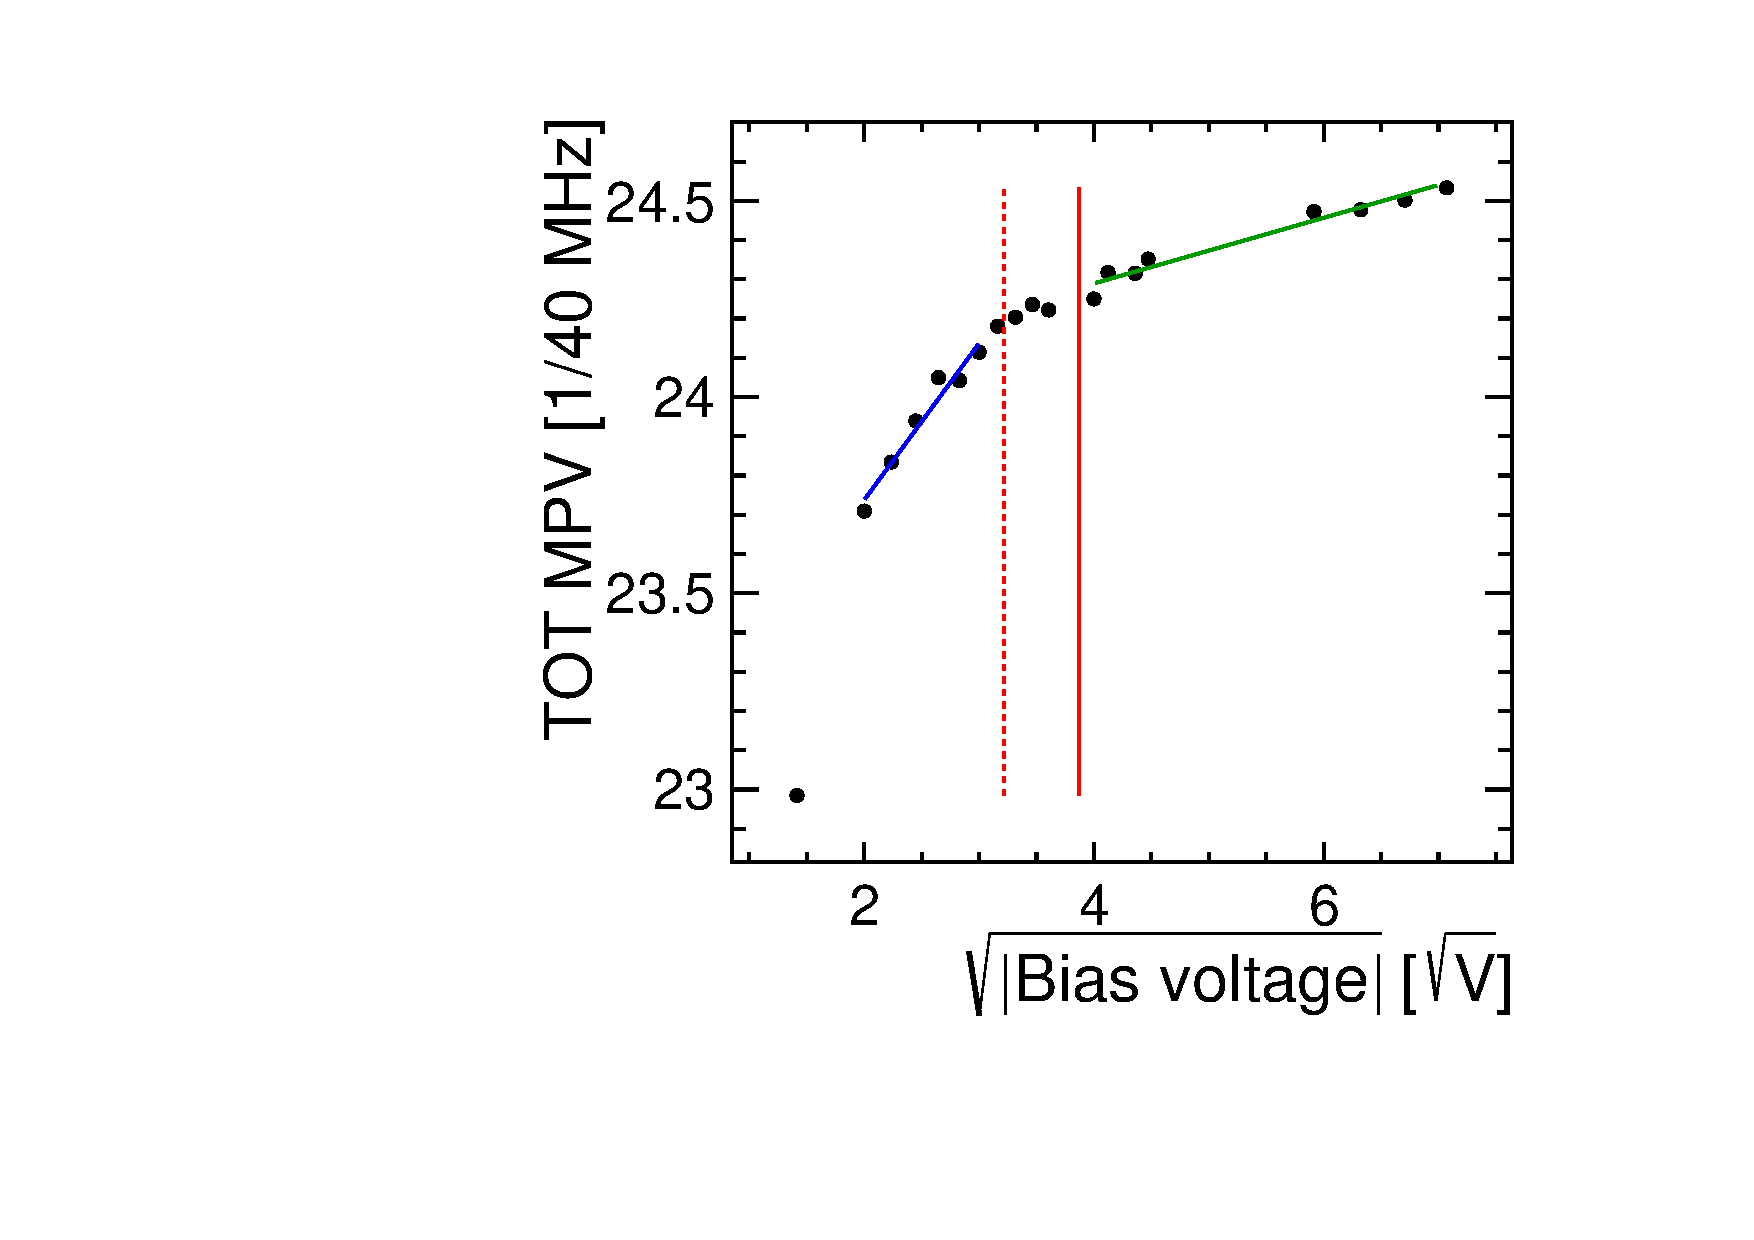
\includegraphics[width=\textwidth]{./figures/TestBeam/depletionVoltage_W0019_G07.pdf}
%%     \caption{}
%%   \end{subfigure}
%%   \caption{20-NGR (W19\_G7): bias and voltage scan.}
%%   \label{fig:Timepix3_THLscan_Vdep_G7}
%% \end{figure}

%% \begin{figure}[htbp] \centering
%%   \begin{subfigure}[b]{0.45\textwidth}
%%     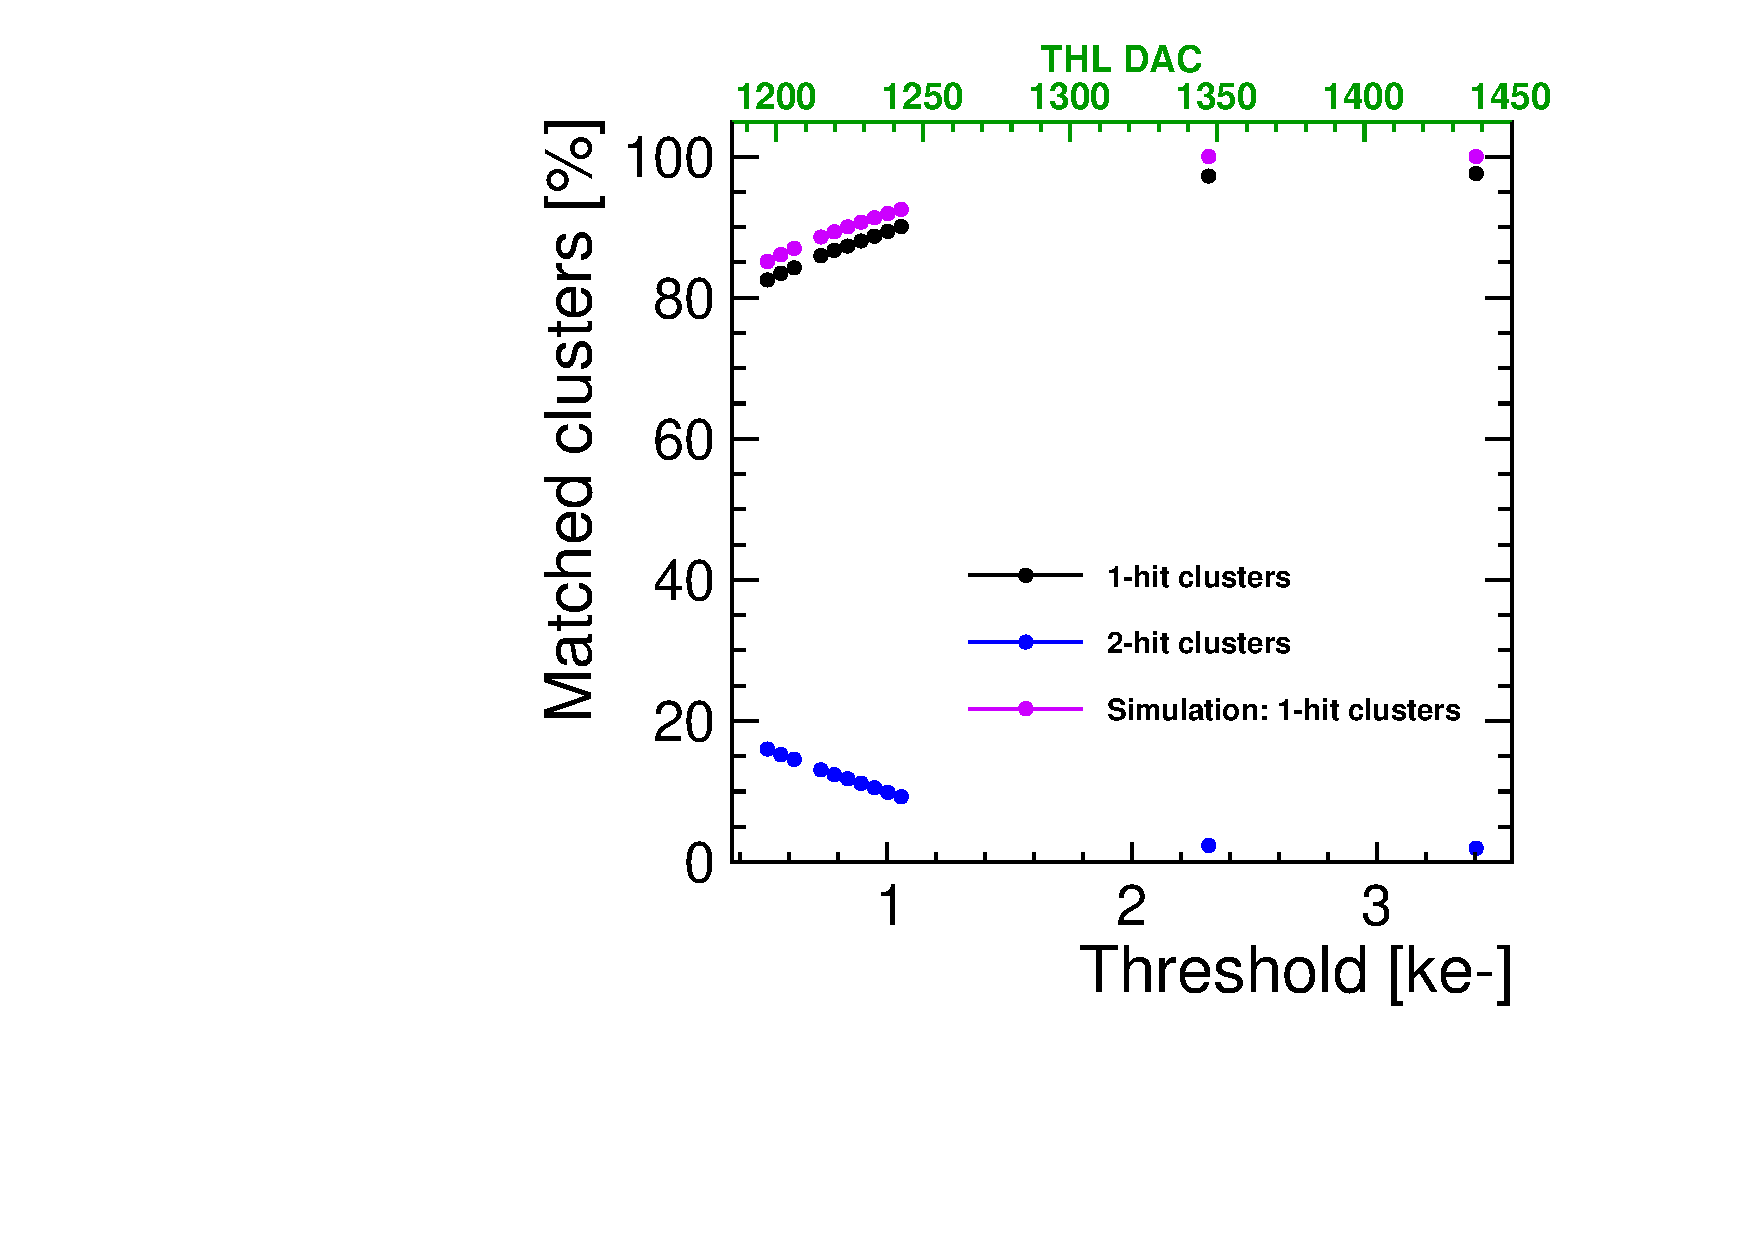
\includegraphics[width=\textwidth]{./figures/TestBeam/ThresholdScan_W0019_F07.pdf}
%%     \caption{}
%%   \end{subfigure} \hfill
%%   \begin{subfigure}[b]{0.45\textwidth}
%%     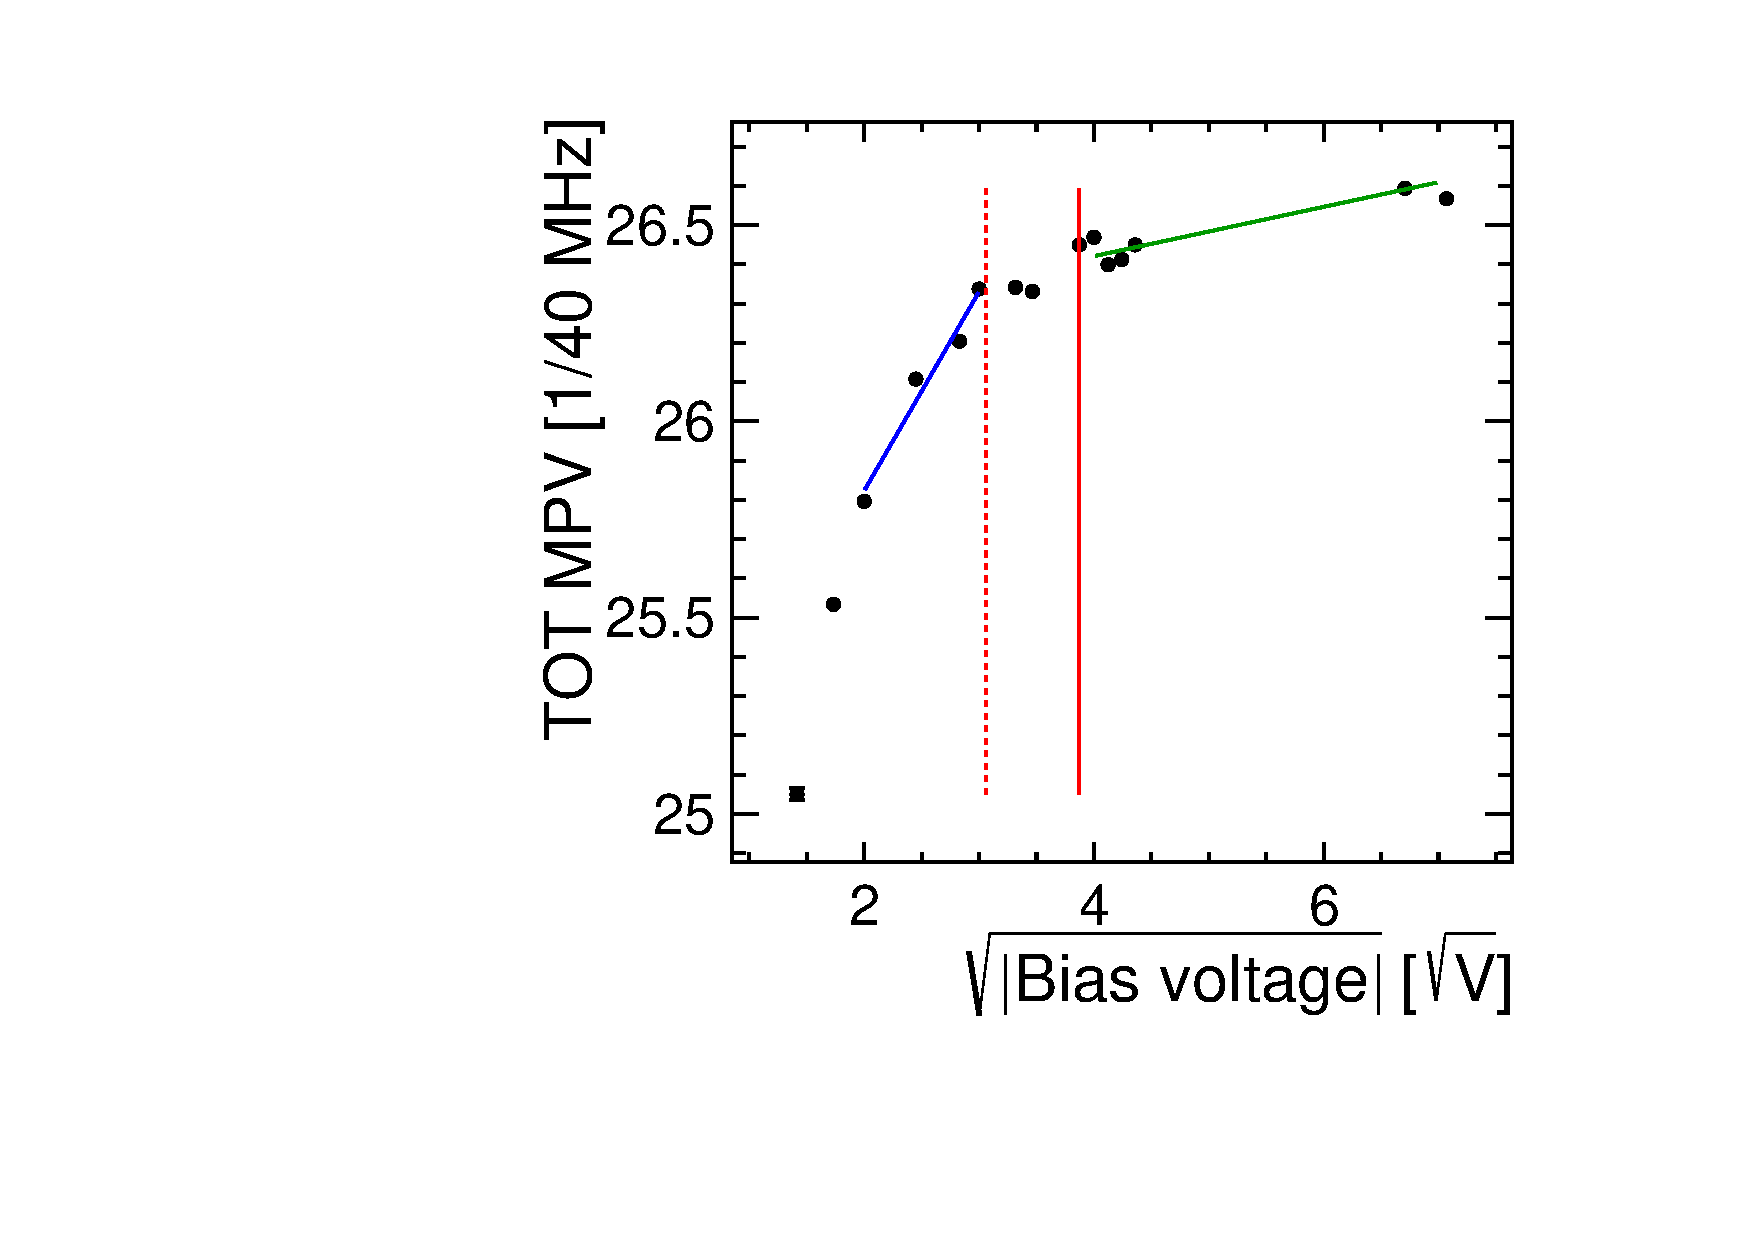
\includegraphics[width=\textwidth]{./figures/TestBeam/depletionVoltage_W0019_F07.pdf}
%%     \caption{}
%%   \end{subfigure}
%%   \caption{23-FGR (W19\_F7): bias and voltage scan.}
%%   \label{fig:Timepix3_THLscan_Vdep_F7}
%% \end{figure}

%% \begin{figure}[htbp] \centering
%%   \begin{subfigure}[b]{0.45\textwidth}
%%     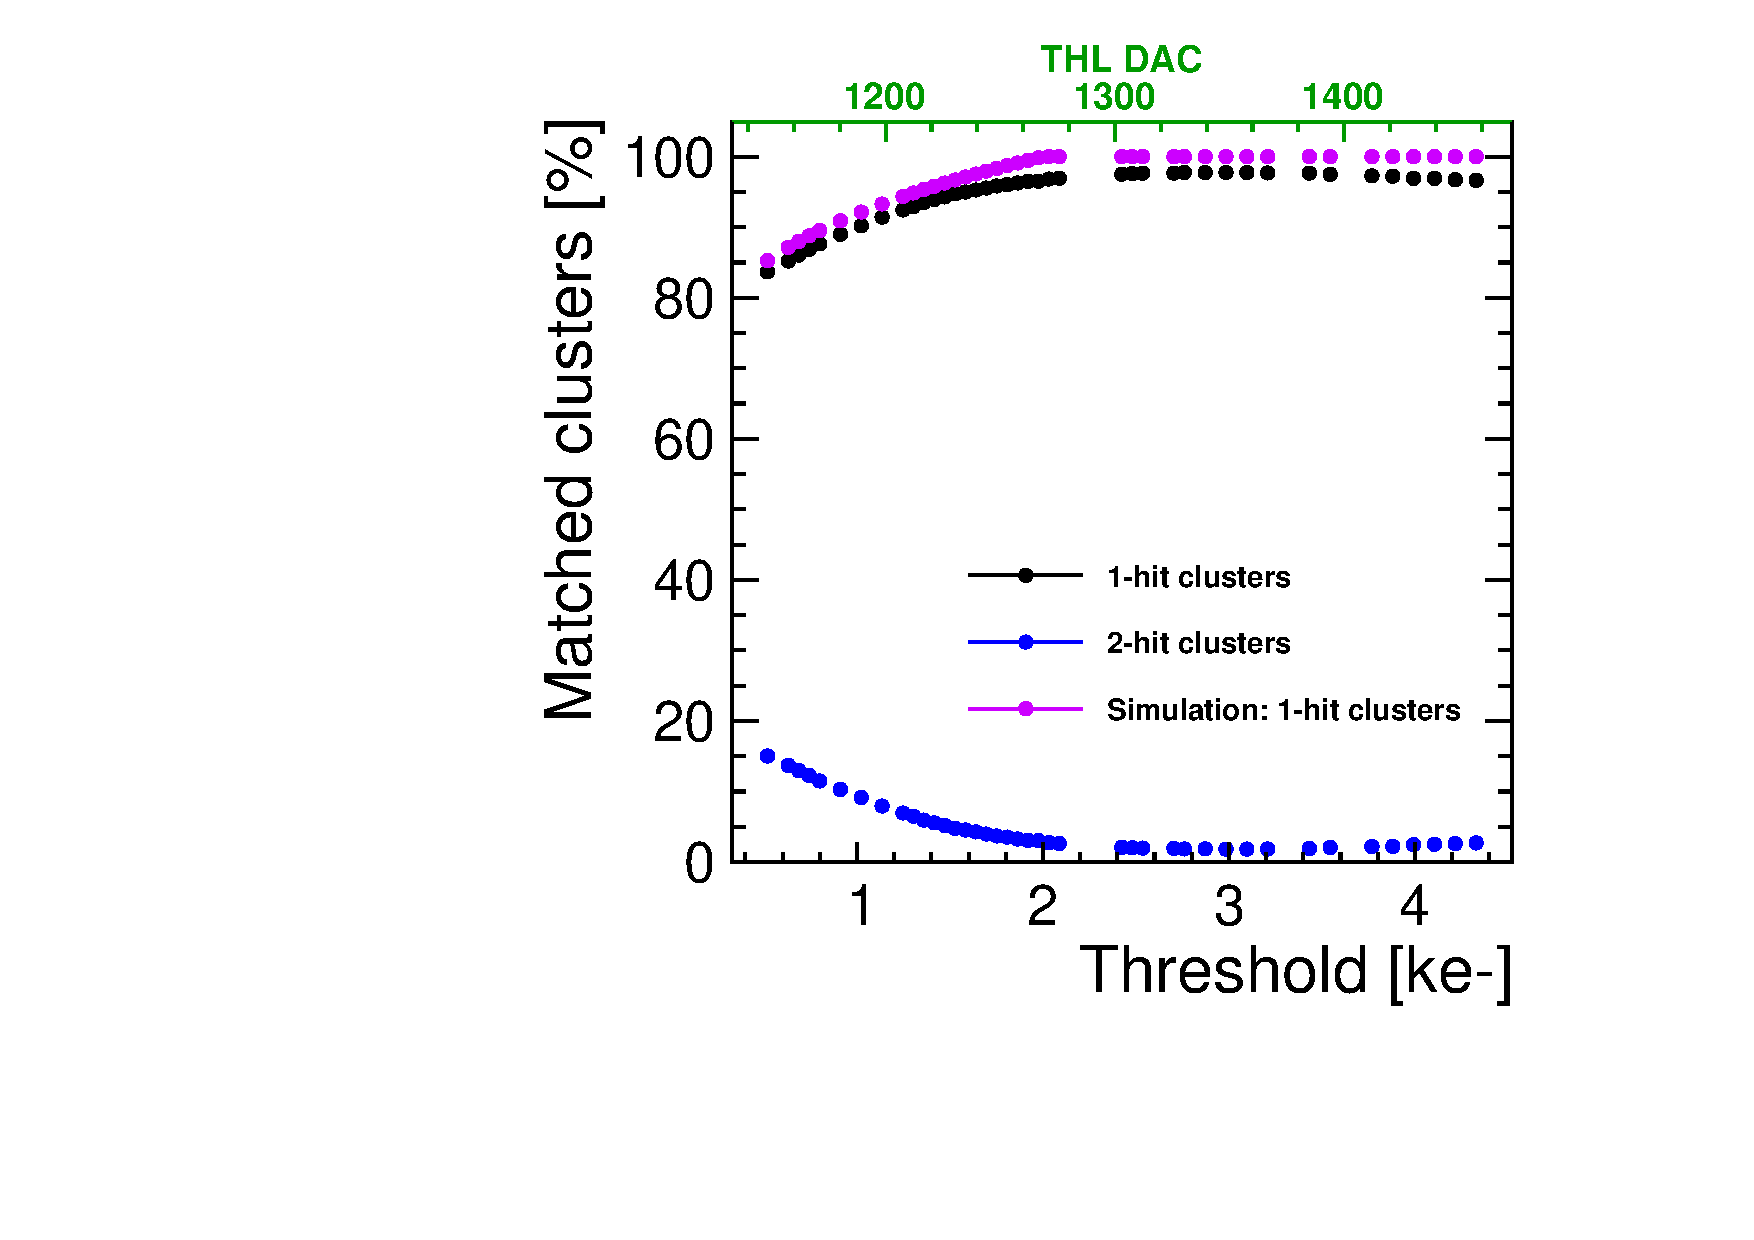
\includegraphics[width=\textwidth]{./figures/TestBeam/ThresholdScan_W0019_L08.pdf}
%%     \caption{}
%%   \end{subfigure} \hfill
%%   \begin{subfigure}[b]{0.45\textwidth}
%%     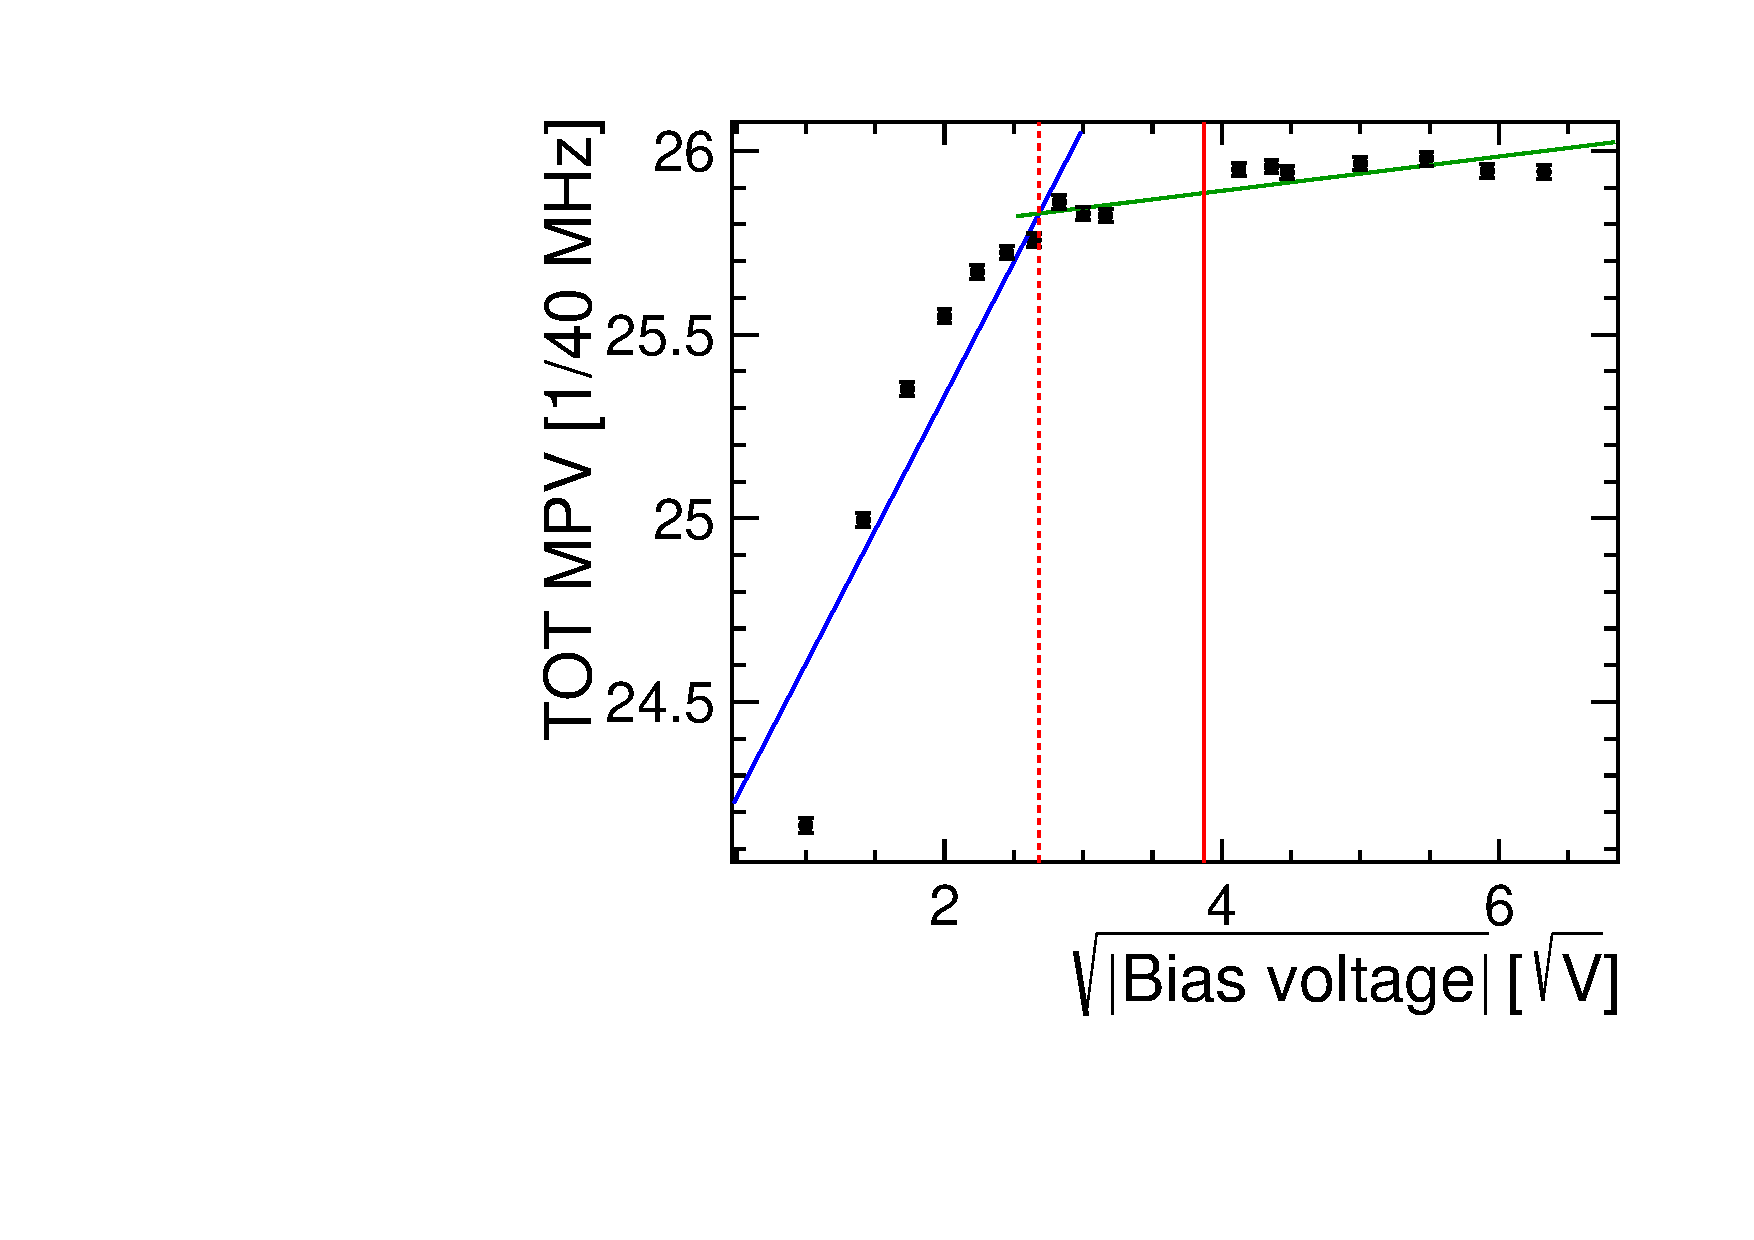
\includegraphics[width=\textwidth]{./figures/TestBeam/depletionVoltage_W0019_L08.pdf}
%%     \caption{}
%%   \end{subfigure}
%%   \caption{28-GNDGR (W19\_L8): bias and voltage scan.}
%%   \label{fig:Timepix3_THLscan_Vdep_L8}
%% \end{figure}


%% \begin{figure}[htbp] \centering
%%   \begin{subfigure}[b]{0.45\textwidth}
%%     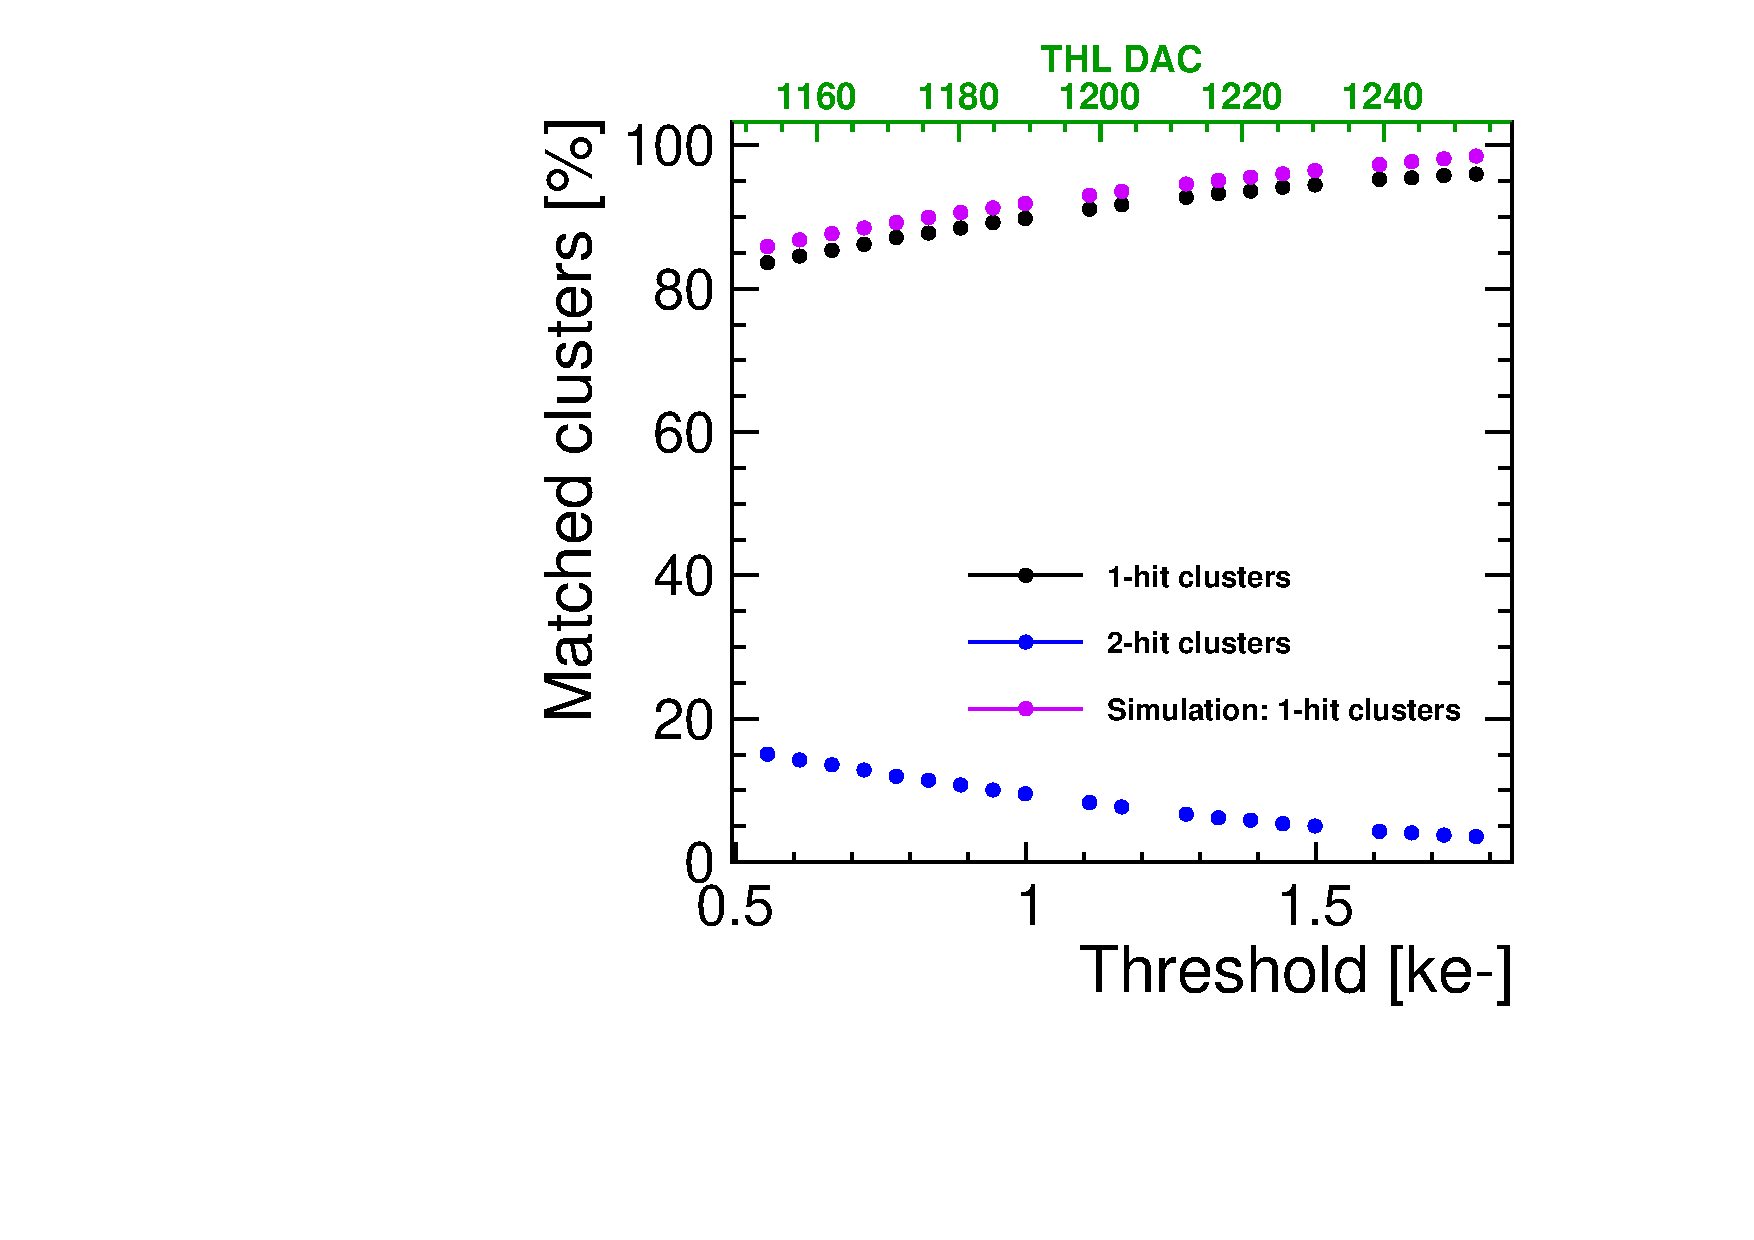
\includegraphics[width=\textwidth]{./figures/TestBeam/ThresholdScan_W0019_C07.pdf}
%%     \caption{}
%%   \end{subfigure} \hfill
%%   \begin{subfigure}[b]{0.45\textwidth}
%%     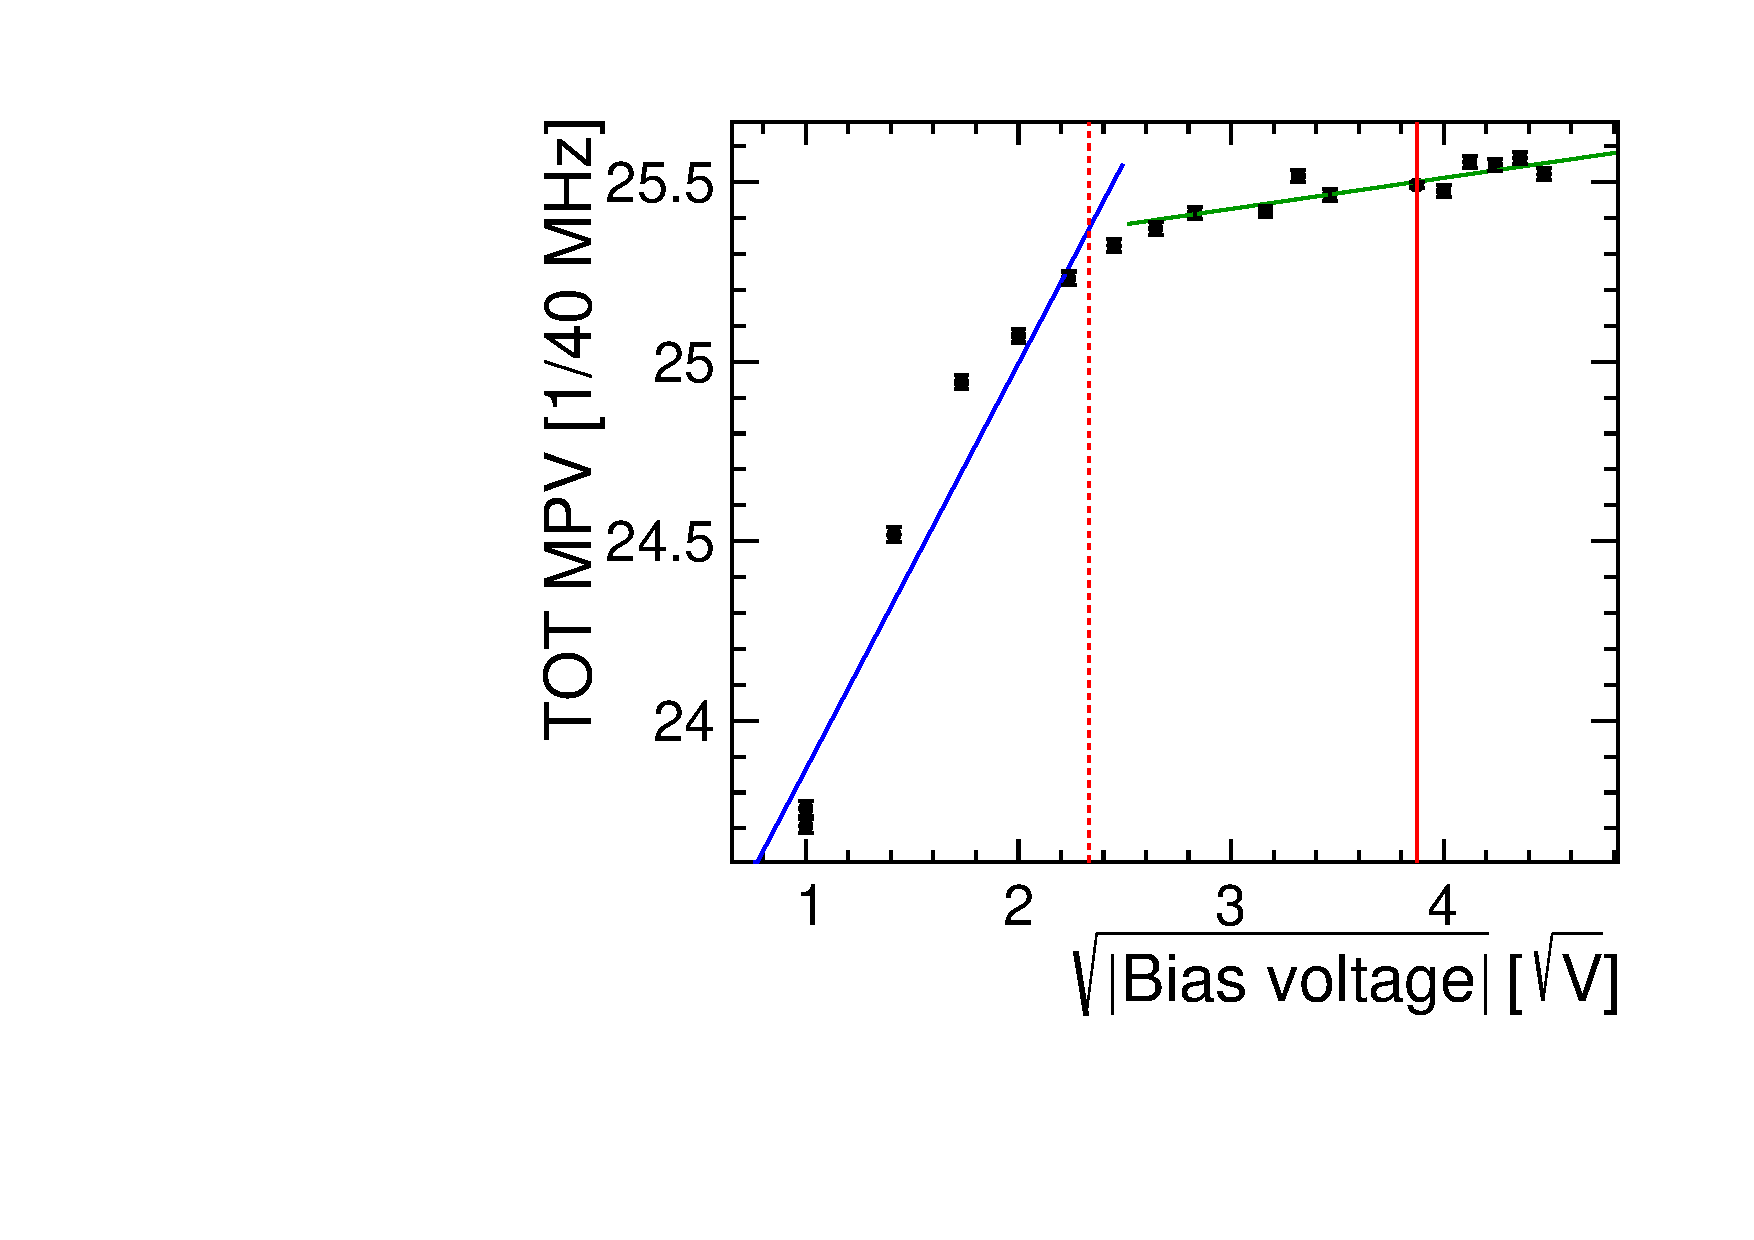
\includegraphics[width=\textwidth]{./figures/TestBeam/depletionVoltage_W0019_C07.pdf}
%%     \caption{}
%%   \end{subfigure}
%%   \caption{55-GNDGR (W19\_C7): bias and voltage scan.}
%%   \label{fig:Timepix3_THLscan_Vdep_C7}
%% \end{figure}

%% \begin{figure}[htbp] \centering
%%   \begin{subfigure}[b]{0.45\textwidth}
%%     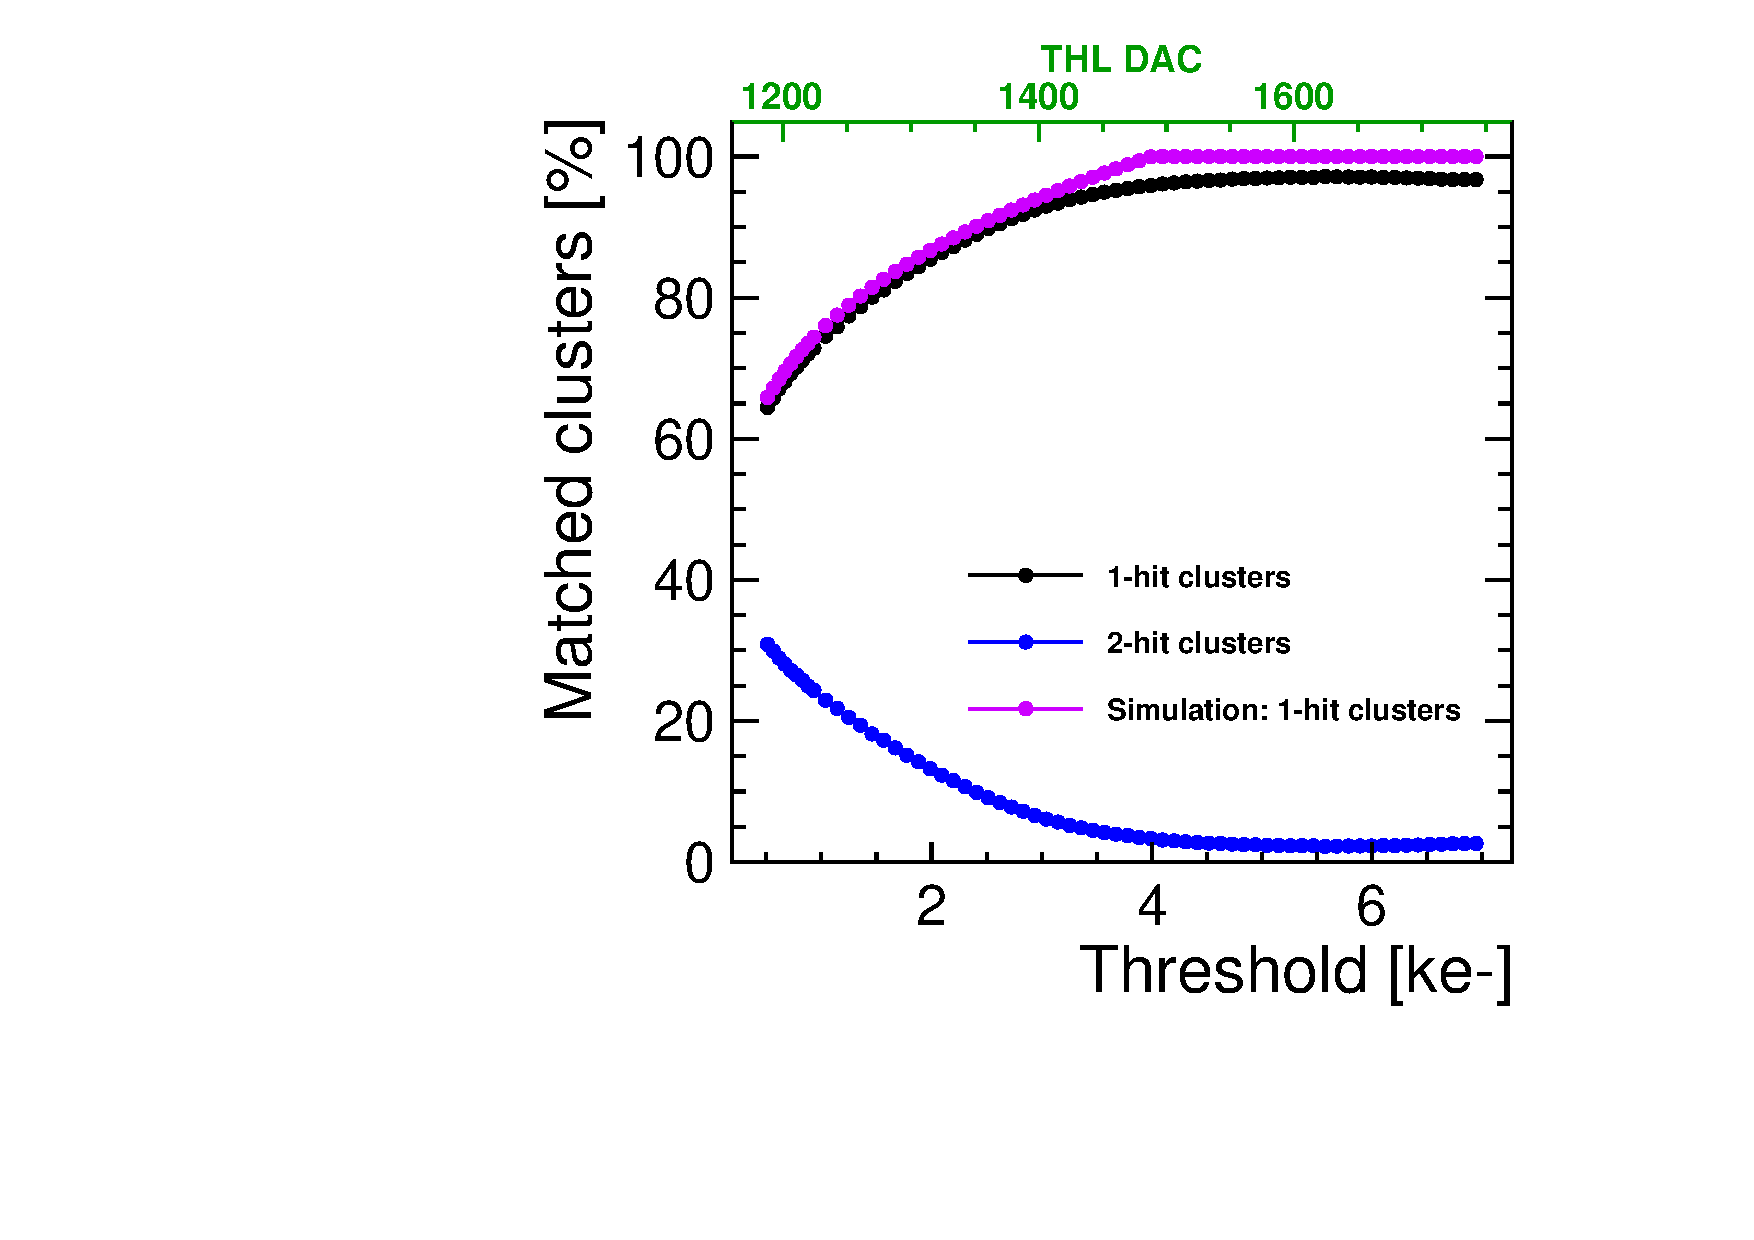
\includegraphics[width=\textwidth]{./figures/TestBeam/ThresholdScan_W0005_E02.pdf}
%%     \caption{}
%%   \end{subfigure} \hfill
%%   \begin{subfigure}[b]{0.45\textwidth}
%%     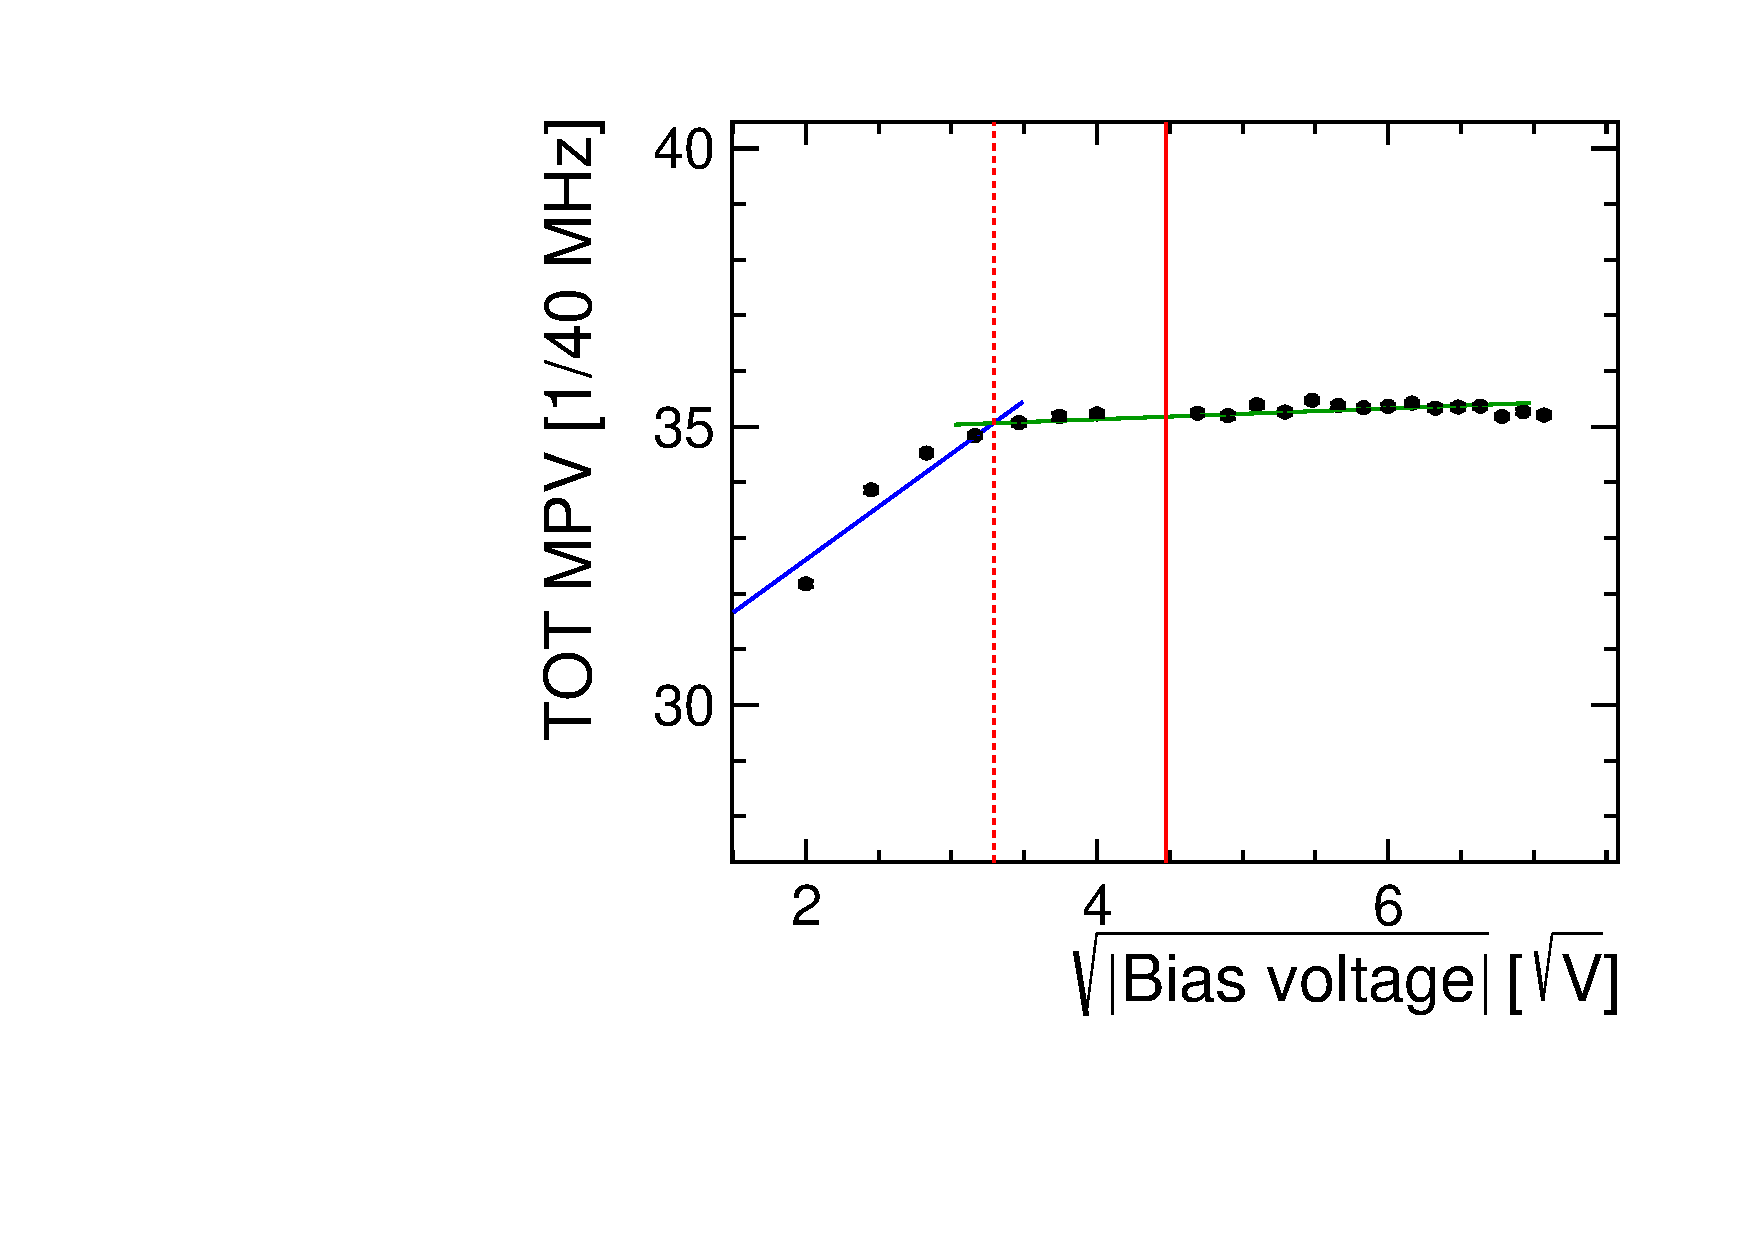
\includegraphics[width=\textwidth]{./figures/TestBeam/depletionVoltage_W0005_E02.pdf}
%%     \caption{}
%%   \end{subfigure}
%%   \caption{55-GNDGR-100 (W5\_E2): bias and voltage scan.}
%%   \label{fig:Timepix3_THLscan_Vdep_E2}
%% \end{figure}


%% \begin{figure}[htbp] \centering
%%   \begin{subfigure}[b]{0.45\textwidth}
%%     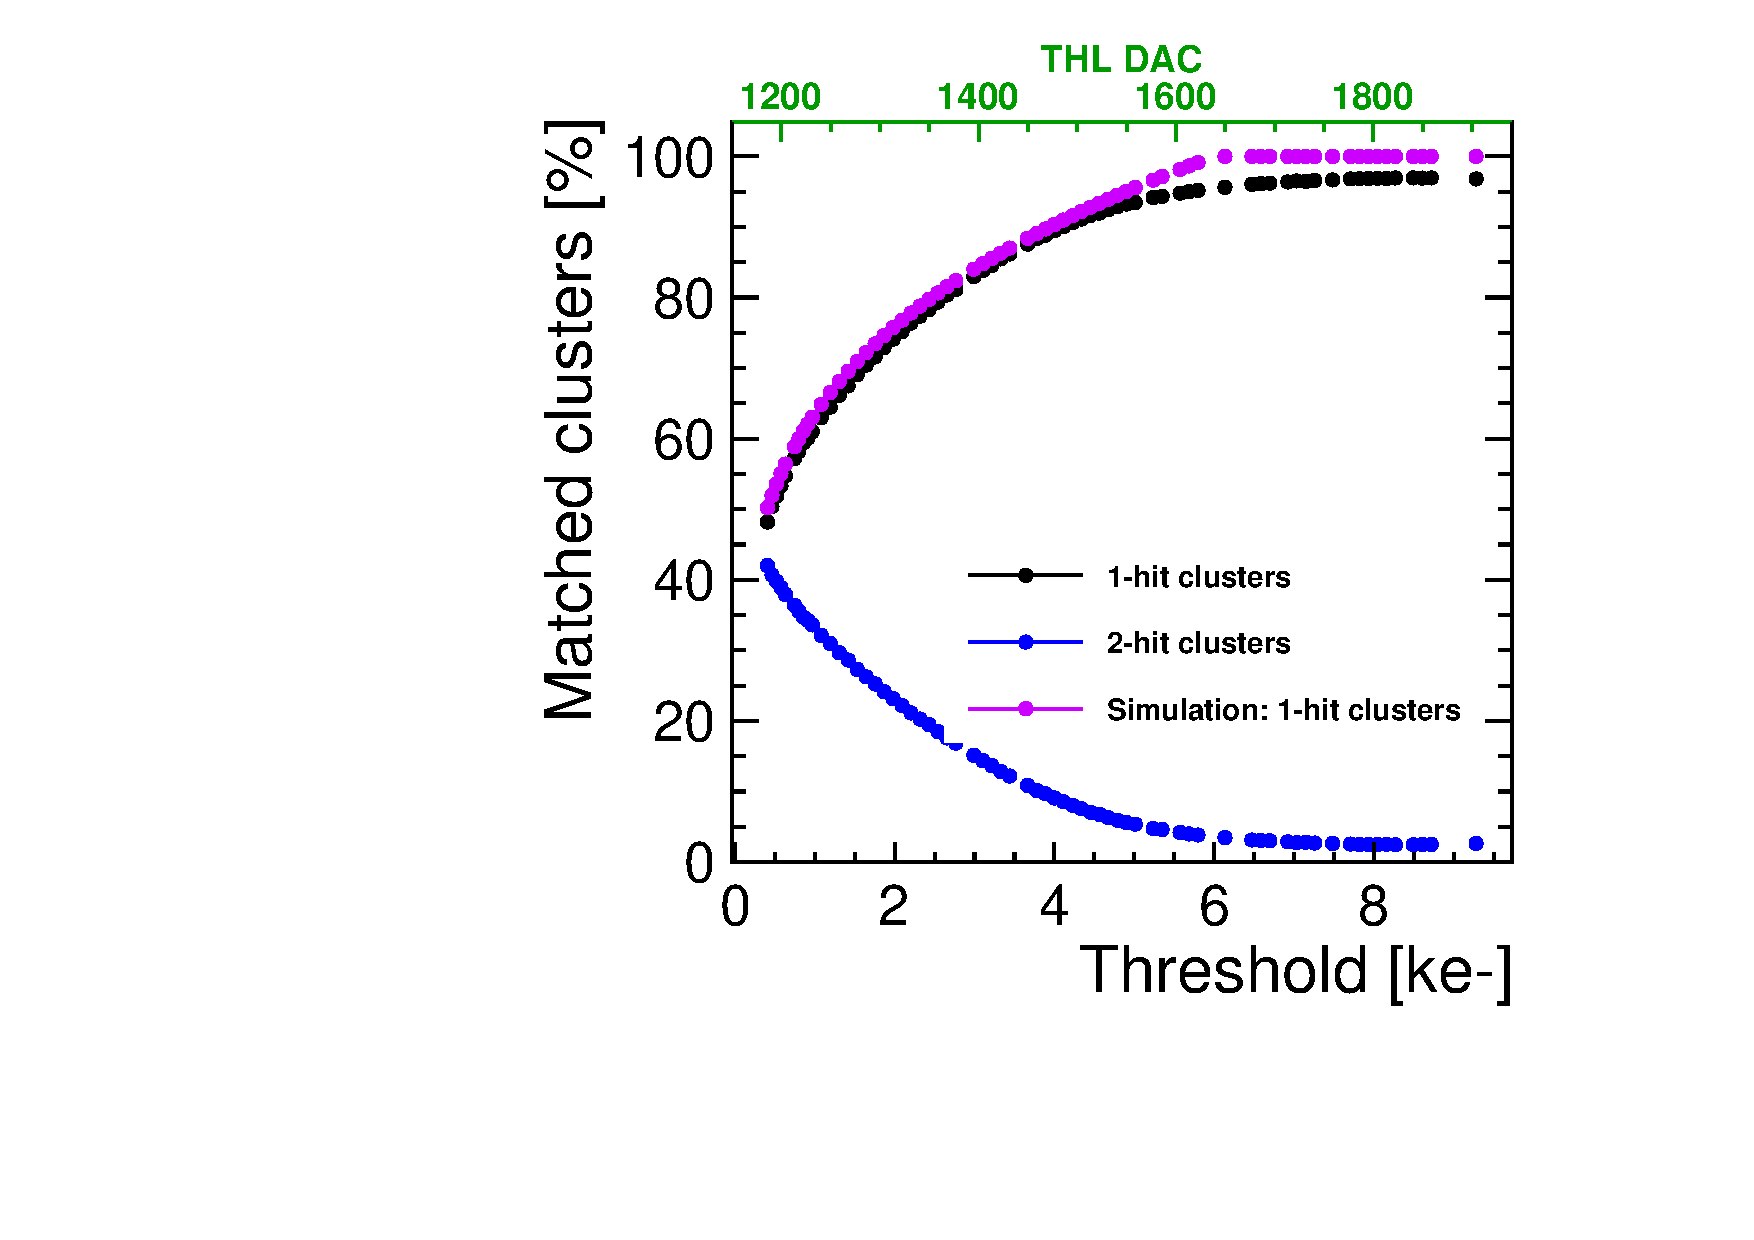
\includegraphics[width=\textwidth]{./figures/TestBeam/ThresholdScan_W0005_F01.pdf}
%%     \caption{}
%%   \end{subfigure} \hfill
%%   \begin{subfigure}[b]{0.45\textwidth}
%%     \includegraphics[width=\textwidth]{./figures/TestBeam/depletionVoltage_W0005_F01.pdf}
%%     \caption{}
%%   \end{subfigure}
%%   \caption{55-GNDGR-150 (W5\_F1): bias and voltage scan.}
%%   \label{fig:Timepix3_THLscan_Vdep_F1}
%% \end{figure}




%% \begin{table}[htbp]
%%   \centering
%%   \caption{Measured depletion voltage for the assemblies described in
%%     \cref{tab:Timepix3Assemblies} and calculated by fitting the
%%     plateau and slope regions of TOT as a function of bias voltage.}
%%   \label{tab:depletionVoltage}
%%   \begin{tabular}{lcccc}
%%     \toprule
%%     Assembly & Thickness [\micron] & Sensor type & Nominal voltage [V] & Depletion voltage [V] \\
%%     \midrule
%%     20-NGR  & 50 & n-in-p & -15 & $<$-9.47 \\
%%     23-FGR & 50 & n-in-p & -15 & $<$-6.32 \\
%%     28-GNDGR & 50 & n-in-p & -15 & $<$-7.19\\
%%     55-GNDGR & 50 & n-in-p & -15 & $<$-5.43\\ \hline
%%     55-GNDGR-100 & 100 & n-in-p & -20 & -10.82 \\ \hline
%%     55-GNDGR-150 & 150 & n-in-p & -30 & -14.86 \\ \hline
%%     W2\_J5       & 300 & p-in-n & 100 & 63.23 \\ 
%%     \bottomrule
%%   \end{tabular}
%% \end{table}


%% \begin{table}[htbp]
%%   \centering
%%   \caption{Measured depletion voltage}
%%   \label{tab:depletionVoltage}
%%   \begin{tabular}{lcccc}
%%     \toprule
%%     Assembly & Thickness [\micron] & Sensor type & Nominal voltage [V] & Depletion voltage [V] \\
%%     \midrule
%%     20-NGR  & 50 & n-in-p & -15 & $<$-9.47 \\
%%     23-FGR & 50 & n-in-p & -15 & $<$-6.32 \\
%%     28-GNDGR & 50 & n-in-p & -15 & $<$-7.19\\
%%     55-GNDGR & 50 & n-in-p & -15 & $<$-5.43\\ \hline
%%     55-GNDGR-100 & 100 & n-in-p & -20 & -10.82 \\ \hline
%%     55-GNDGR-150 & 150 & n-in-p & -30 & -14.86 \\ \hline
%%     W2\_J5       & 300 & p-in-n & 100 & 63.23 \\ 
%%     \bottomrule
%%   \end{tabular}
%% \end{table}


%%%%\subsection{Resolution vs. thickness}
% \begin{figure}[htbp] \centering
%   \begin{subfigure}[b]{0.45\textwidth}
%     \includegraphics[width=\textwidth]{./figures/TestBeam/cluSize_vs_thickness.pdf}
%     \caption{}
%   \end{subfigure} \hfill
%   \begin{subfigure}[b]{0.45\textwidth}
%     \includegraphics[width=\textwidth]{./figures/TestBeam/residuals_vs_thickness.pdf}
%     \caption{}
%   \end{subfigure}
%   \caption{Cluster size and residuals vs. thickness (run 2003 for 300 um thick sensor was taken at 70 V).}
%   \label{fig:clusize_residuals_vs_thickness}
% \end{figure}


%% \begin{figure}[htbp] \centering
%%   \begin{subfigure}[b]{0.3\textwidth}
%%     \includegraphics[width=\textwidth]{figures/TestBeam/50micron_sizeX.pdf}
%%     \caption{}
%%   \end{subfigure} \hfill
%%   \begin{subfigure}[b]{0.3\textwidth}
%%     \includegraphics[width=\textwidth]{figures/TestBeam/50micron_resX.pdf}
%%     \caption{}
%%   \end{subfigure} \hfill
%%   \begin{subfigure}[b]{0.3\textwidth}
%%     \includegraphics[width=\textwidth]{figures/TestBeam/50micron_Edep.pdf}
%%     \caption{}
%%   \end{subfigure}
%%   \caption{For $50\,\micron$ thick sensor.}
%%   \label{fig:G4_simu_data_50micron}
%% \end{figure}

%% \begin{figure}[htbp] \centering
%%   \begin{subfigure}[b]{0.3\textwidth}
%%     \includegraphics[width=\textwidth]{figures/TestBeam/100micron_sizeX.pdf}
%%     \caption{}
%%   \end{subfigure} \hfill
%%   \begin{subfigure}[b]{0.3\textwidth}
%%     \includegraphics[width=\textwidth]{figures/TestBeam/100micron_resX.pdf}
%%     \caption{}
%%   \end{subfigure} \hfill
%%   \begin{subfigure}[b]{0.3\textwidth}
%%     \includegraphics[width=\textwidth]{figures/TestBeam/100micron_Edep.pdf}
%%     \caption{}
%%   \end{subfigure}
%%   \caption{For $100\,\micron$ thick sensor.}
%%   \label{fig:G4_simu_data_100micron}
%% \end{figure}

%% \begin{figure}[htbp] \centering
%%   \begin{subfigure}[b]{0.3\textwidth}
%%     \includegraphics[width=\textwidth]{figures/TestBeam/150micron_sizeX.pdf}
%%     \caption{}
%%   \end{subfigure} \hfill
%%   \begin{subfigure}[b]{0.3\textwidth}
%%     \includegraphics[width=\textwidth]{figures/TestBeam/150micron_resX.pdf}
%%     \caption{}
%%   \end{subfigure} \hfill
%%   \begin{subfigure}[b]{0.3\textwidth}
%%     \includegraphics[width=\textwidth]{figures/TestBeam/150micron_Edep.pdf}
%%     \caption{}
%%   \end{subfigure}
%%   \caption{For $150\,\micron$ thick sensor.}
%%   \label{fig:G4_simu_data_150micron}
%% \end{figure}


%%%%% CALIBRATION vs. GEANT4
% \cref{sec:testBeamDataCalibrated_vs_G4} compares the
% calibrated data with the \textsc{Geant4} energy deposition using the
% PAI physics list (c.f. \cref{sec:Silicon_Geant4}) for $50\,\micron$,
% $100\,\micron$ and $150\,\micron$ thick planar sensors. There is a
% good agreement in terms of the most probable value (MPV) and the
% full-width-at-half-maximum (FWHM) in both simulation and data.
% \begin{figure}[htbp] \centering
%   \begin{subfigure}[b]{0.33\textwidth}
%     \includegraphics[width=\textwidth]{./figures/Calibration/Edep_G4_W0019_G07.pdf}
%     \caption{55-GNDGR}
%   \end{subfigure} \hfill
%   \begin{subfigure}[b]{0.33\textwidth}
%     \includegraphics[width=\textwidth]{./figures/Calibration/Edep_G4_W0005_E02.pdf}
%     \caption{55-GNDGR-100}
%   \end{subfigure}\hfill
%   \begin{subfigure}[b]{0.33\textwidth}
%     \includegraphics[width=\textwidth]{./figures/Calibration/Edep_G4_W0005_F01.pdf}
%     \caption{55-GNDGR-150}
%   \end{subfigure}
%   \caption{Calibrated energy distribution of test beam data for
%     different assemblies. The pixel-by-pixel calibration is applied to
%     the data which is obtained using test pulses. \textsc{Geant4}
%     energy deposition is obtained using the PAI physics list.}
%   \label{sec:testBeamDataCalibrated_vs_G4}
% \end{figure}
